\documentclass[a4paper,11pt,hyperfootnotes]{article}
\usepackage[utf8]{inputenc}
\usepackage[font={small}, bf]{caption}
\usepackage{hyperref}
\usepackage[]{fullpage}
\usepackage[titletoc,title]{appendix}
\usepackage{listings}
% \usepackage{gloss}
\newcommand\nil{\varnothing}
% \newcommand\defeq{:=}
\newcommand\defeq{\overset{\textrm{\tiny def}}{=}}
\newcommand\Xor{\underset{\textbf{\Large--}}{\bigvee}}
\providecommand{\xor}{\veebar}
\usepackage{amsmath}
\usepackage{amssymb}
\usepackage{amsthm}
\usepackage{thmtools}
\declaretheoremstyle[
spaceabove=8pt, spacebelow=8pt,headfont=\normalfont\bfseries,headpunct={.\\},notefont=\bfseries, notebraces={ -- }{},bodyfont=\normalfont,postheadspace=4pt,qed={}]{theorem}
% \newtheorem{definition}{Definition}
% \newtheorem{corollary}[definition]{Corollary}
% \newtheorem{theorem}[definition]{Theorem}
% \newtheorem{lemma}[definition]{Lemma}

\declaretheorem[style=theorem]{theorem}
\declaretheorem[style=theorem,sibling=theorem]{definition}
\declaretheorem[style=theorem,sibling=theorem]{corollary}
\declaretheorem[style=theorem,sibling=theorem]{lemma}
\setcounter{tocdepth}{2}
\setcounter{secnumdepth}{2}
\DeclareMathOperator{\concat}{\operatorname{\oplus}}
\DeclareMathOperator{\Concat}{\operatornamewithlimits{\bigoplus}}
\DeclareMathOperator{\rangedel}{:}
% \DeclareMathOperator{\xor}{:}
\usepackage{enumitem}
\usepackage{tikz}
\usetikzlibrary{matrix,arrows.meta,fit,positioning,shapes,automata}
\usepackage{forest}
\usepackage{graphicx}
% \makeatletter
% \def\ll@definition{%
%   \protect\numberline{\csname the\thmt@envname\endcsname}%
%   \ifx\@empty\thmt@shortoptarg
%     \thmt@thmname
%   \else
%     \thmt@shortoptarg
%   \fi}
% \def\l@thmt@definition{} 
% \makeatother
\bibliographystyle{apalike}
% statuses in section names
\newif\ifdraft
% \drafttrue % Uncomment to compile whole draft document / comment to compile only finished sections.
% for error explanation see: https://tex.stackexchange.com/questions/64298/error-with-xcolor-package
\usepackage{xcolor}
\colorlet{GREEN}{green}
\colorlet{ORANGE}{orange}
\colorlet{YELLOW}{yellow}
\colorlet{RED}{red}
% none of these work
% \ifdraft
\usepackage{bbding}
\usepackage{pifont}
\newcommand{\cmark}{\ding{51}}%
\newcommand{\xmark}{\ding{55}}%
% \usepackage{unicode-math}
% \newcommand{\cmark}{\setmainfont{Linux Libertine O}\symbol{"2714}\par}
% \newcommand{\xmark}{\setmainfont{Linux Libertine O}\symbol{"2718}\par}
% \usepackage{fontawesome}
% \def\cmark{\FA\symbol{"F00C}}
% \def\xmark{\FA\symbol{"F00D}}
% \fi
% \newcommand{\cmark}{${\checkmark}$}
% \newcommand{\xmark}{${\times}$}
% \newcommand{\cmark}{***}
% \newcommand{\xmark}{xxx}
\newcommand{\validator}[1]{\mathbb{V}^{\textsc{#1}}}
\newcommand{\proofof}[1]{\Pi^{\textsc{#1}}}
\newcommand{\idx}[1]{\texttt{[}\/#1\/\texttt{]}}
\newcommand\statusgreen{\ifdraft \textcolor{green}{\cmark}\fi} 
\newcommand\statusyellow{\ifdraft \textcolor{yellow}{\cmark}\fi} 
\newcommand\statusorange{\ifdraft \textcolor{orange}{\cmark}\fi} 
\newcommand\statusred{\ifdraft \textcolor{red}{\xmark}\fi} 
\newcommand\statuspriority{\ifdraft \textcolor{blue}{PRIORITY}\fi}

%%%%%%%%%%%%%%%%%%%%%%%%%%%%%%%%%%%%%%%%%%%%%%%%%%%%%%%%%%%%%


\renewcommand{\listtheoremname}{}
\usepackage[margin=1cm]{caption}
\usepackage{anyfontsize}
\usepackage{longtable}
\usepackage{parskip}
\usepackage{booktabs}
\setlength{\parindent}{0pt}
\setlength{\parskip}{\baselineskip}

\providecommand{\tightlist}{%
  \setlength{\itemsep}{0pt}\setlength{\parskip}{0pt}}
\usepackage{colortbl}
\ifdefined\Shaded\renewenvironment{Shaded}{\begin{tcolorbox}[frame hidden, sharp corners, enhanced, borderline west={3pt}{0pt}{shadecolor}, boxrule=0pt, interior hidden, breakable]}{\end{tcolorbox}}\fi

\title{\fontsize{28}\Huge\sc 
Future-proof Storage\vskip5pt
\Large economic incentives for sharing storage capacity\vskip1pt\vskip-18pt
to achieve data persistance
\vskip1pt\vskip-18pt
in the Swarm peer to peer network}
%\renewcommand{\abstractname}{\ }
\author{Swarm Research Division%
\thanks{Viktor Trón, Ábel Bodó, Rinke Hendriksen,  Dániel A. Nagy, Daniel Nickless, Gyuri Barabás, Viktor Tóth, Mark Bliss, Callum Toner, Peter Mrekaj, Esad Akar, Alok Nerurkar, Anatol Lupacescu, Áron Fischer.}
\thanks{The authors thank Houhuli Silur for their thorough review of this work and suggestions for improvement.
}}
\date{v5.4 - may the fourth bee with you 2023
\vskip35pt
\includegraphics[width=0.15\textwidth]{fig/logo.pdf}
}
\begin{document}
\maketitle
\begin{abstract}
\noindent Swarm is a peer-to-peer network of nodes that collectively provide a decentralised storage and communication solution.  Its built-in incentive system is enforced through smart contracts on the Ethereum blockchain and powered by the BZZ token. While individual nodes are assumed to pursue selfish strategies that maximise their operator's profit, the behaviour of the network as a whole attains emergent properties in alignment with the requirements of such a cloud service.

\medskip

\noindent In this paper, we present a novel solution to make decentralised storage economically self-sustaining. First, we introduce Swarm's basic DISC model of storage and distribution with incentives for bandwidth sharing. Then we describe the system of postage stamps as a costly signal that lets users indicate priority of storage. The smart contract that implements this system lets users purchase postage stamps in batches and accumulates the revenue which serves as the pot to redistribute among storage providers to incentivise the contribution of their disc space. This redistribution is managed by  a set of smart contracts implementing a  system of probabilistic outpayments, called the redistribution game. Genuine storers can claim their reward through the  contract. Part of the evidence that storers provide as proof of entitlement to the reward can be interpreted as signals of demand and supply. These are responded to by automatic price updates, which makes, in turn, storage provision a self-regulating market.
\end{abstract}

\newpage

\tableofcontents

\newpage

\listoffigures
\listoftables
\newpage

In section \ref{sec:disc}, we introduce Swarm's DISC model to set the scene for the incentives. Section \ref{sec:postage-stamps} discusses postage stamps from the  users and the ecosystem's perspective.  In section \ref{sec:redistribution} we describe a redistribution scheme that enables direct payout from the proceeds of the postage stamps and thereby distributes postage revenue  to storage providers fairly. 

\section{The DISC model}\label{sec:disc}

In this section we briefly outline Swarm's underlying storage model, and discuss how rewards for bandwidth sharing already serve as an incentive for storing popular content. We conclude by stating the need for a separate subsystem to reward the sharing of spare storage capacity (i.e., disc space) to preserve content rarely requested.

\subsection{Peer-to-peer storage network}\label{sec:p2p}

The DISC (\/\emph{Distributed Immutable Store of Chunks}) is the storage layer underlying Swarm. 
The canonical unit of storage in Swarm is called a \emph{chunk} (see definition \ref{def:cac} in appendix \ref{sec:appendix-disc}). A chunk consists of at most 4 kilobytes of data and has an address. Chunks are created through a higher-level upload mechanism that splits files and generates an index in such a way that the files can be reassembled upon download. Since a chunk’s address is taken from the same address space as a node’s address, it is possible to compute their \emph{proximity} using an xor-based distance metric (see definition \ref{def:xorPO} in appendix \ref{sec:appendix-disc}). The DISC prescribes that each chunk is stored by the nodes with an address that is close to that of the chunk itself. Nodes within some agreed proximity form a \emph{neighbourhood} and share all chunks falling in the address range they cover.

To insert a chunk into the swarm, nodes relay the chunk via the \emph{push-sync protocol} until it arrives at the neighbourhood it belongs to. A \emph{receipt} confirming the storage of the chunk is then passed back  to the uploader along the same route. In order to retrieve a chunk, a request with a chunk address is routed towards the relevant neighbourhood using the retrieval protocol. If any node encountered on the way already has the corresponding chunk in their local storage, the chunk data is sent back as a response. If peers in  the network maintain a connectivity pattern according to a specific topology, such a peer will always exist unless the uploading peer is itself the closest. Therefore, successively relaying to a more proximate peer constitutes a routing strategy that finds a way to the node closest to any address.  Routing from anywhere to the  chunk's neighbourhood provides the basis for the storage and retrieval  of chunks in swarm. 

Neighbours continuously synchronise their chunk storage using the \emph{pull-sync protocol}. This guarantees that all chunks belonging to a neighbourhood are stored by each  node in the corresponding neighbourhood. The redundancy this confers adds resilience in that chunks will remain available even if some of the nodes in the neighbourhood become unreachable. The synchronisation protocol also ensures that the neighbourhood's storage remains consistent as nodes go offline and new nodes join the network. 


Automatic scaling of distribution is enabled because nodes who participate in routing retrieval requests may choose to retain some of the chunks they have relayed back along the request forwarding path. Economic motivation for such \emph{opportunistic caching} is provided by the bandwidth incentives.



\begin{figure}[!th]
  \centering
    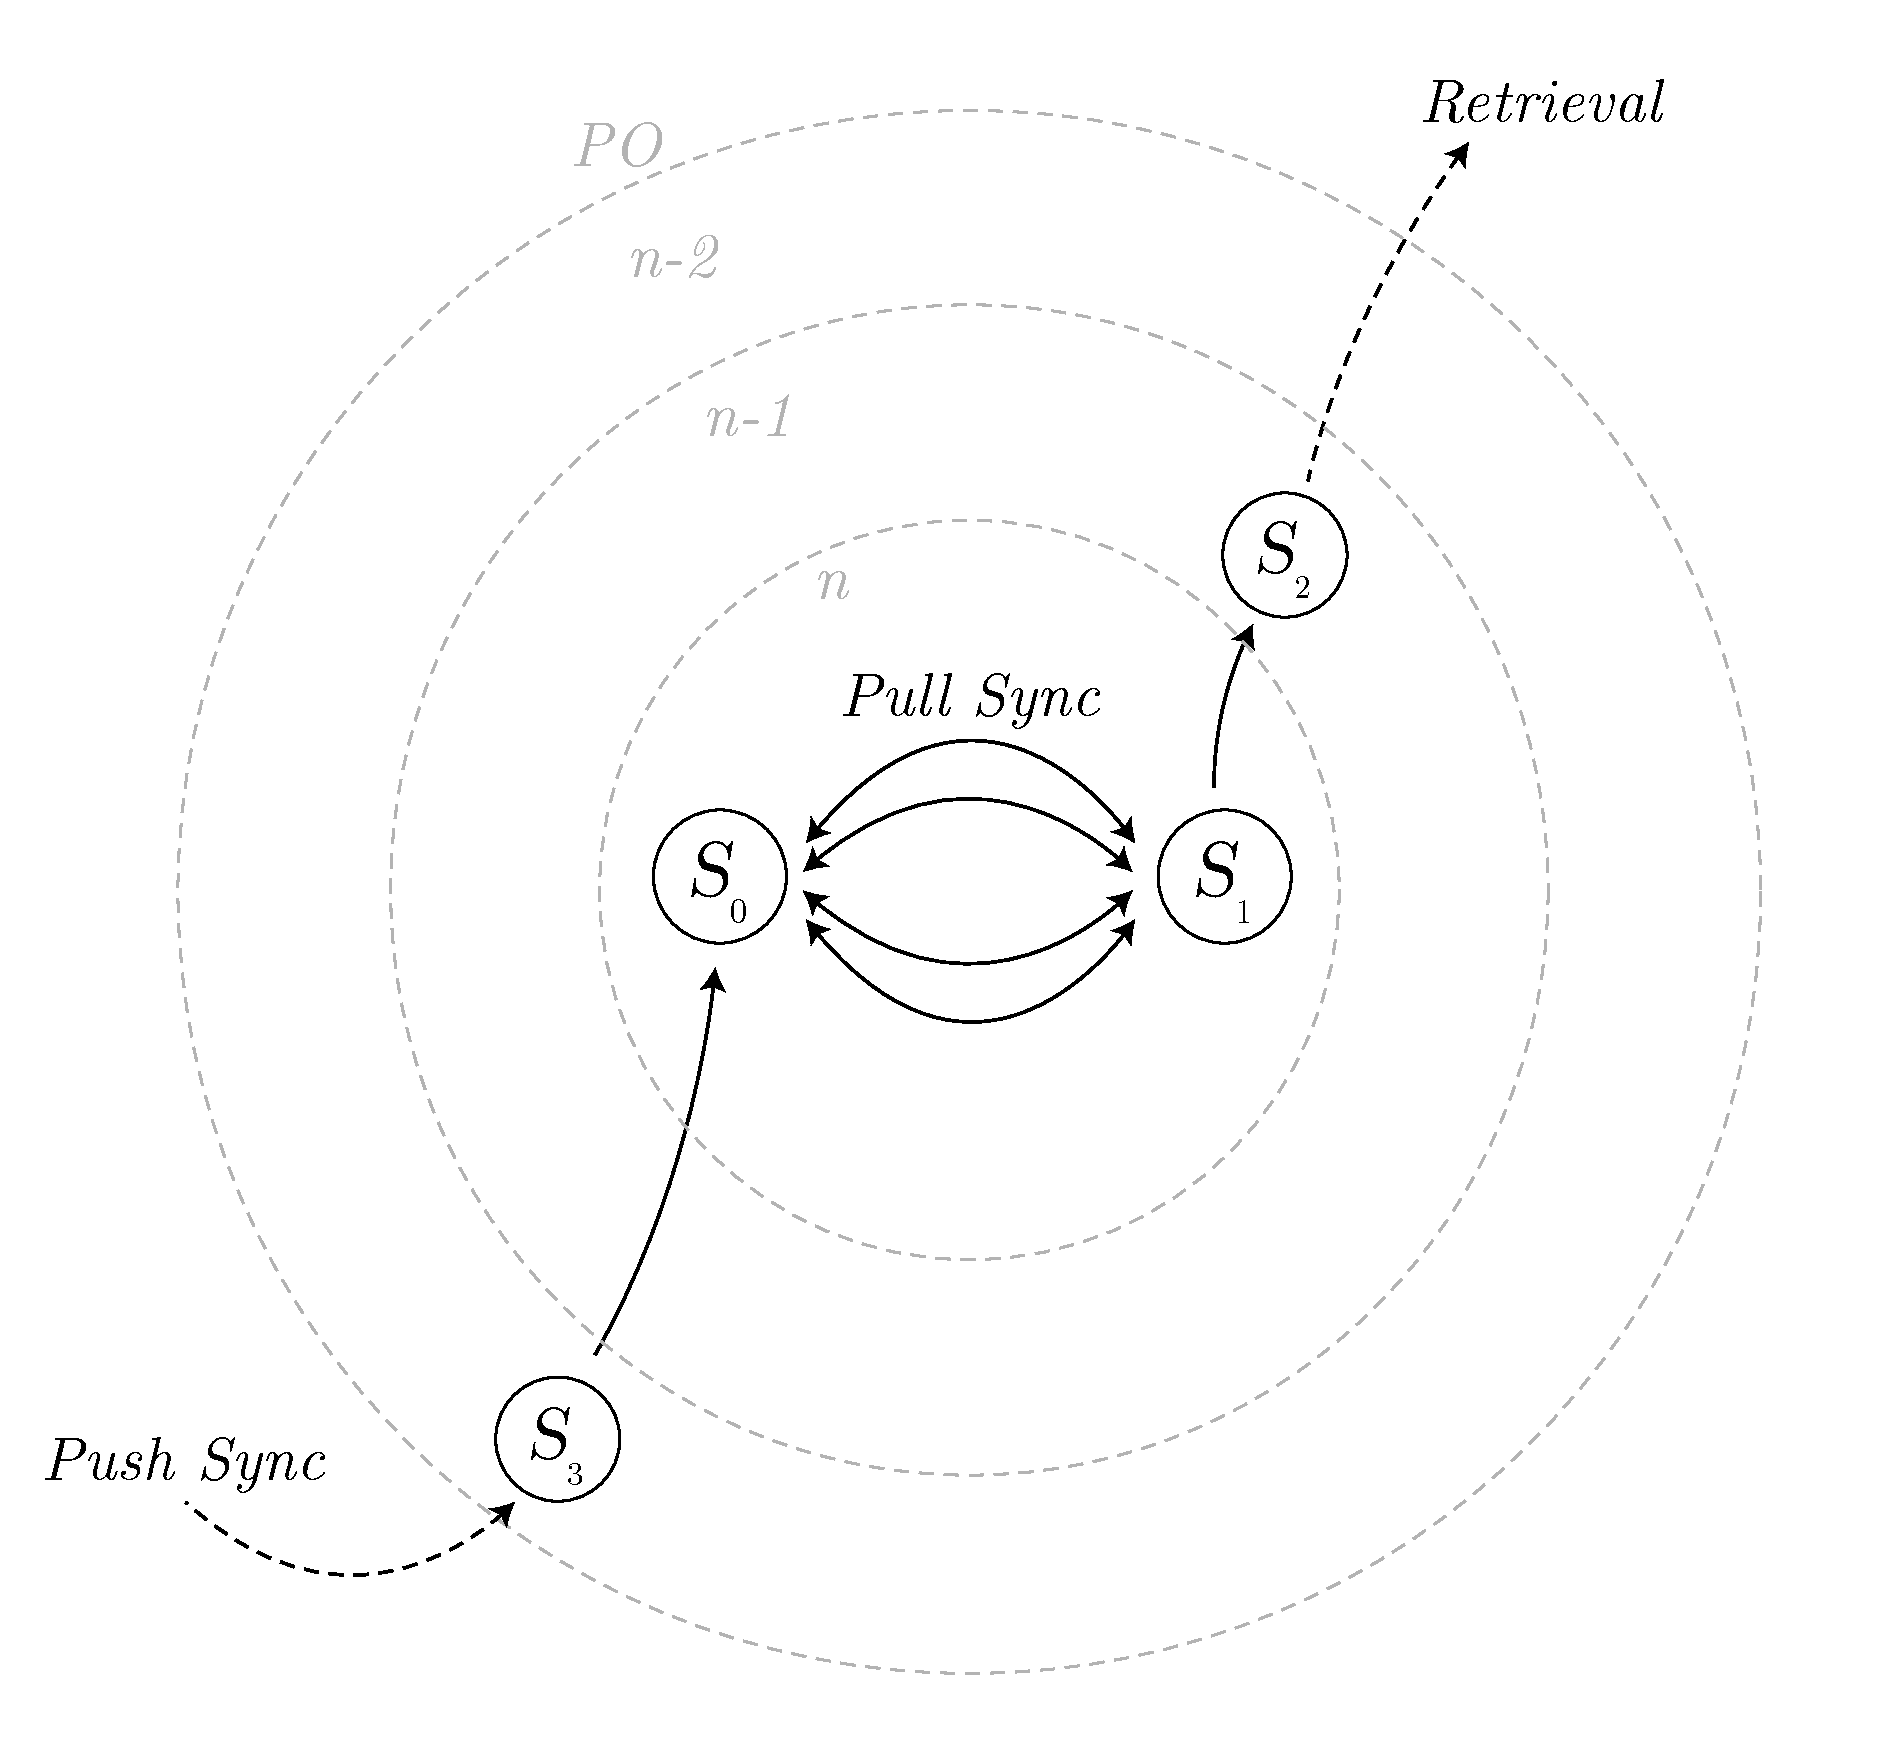
\includegraphics[width=.5\textwidth]{fig/pull-push-retrieve.pdf}
  \caption[Push, Pull and Retrieve Protocols]{Push, Pull and Retrieve Protocols. The figure depicts the typical trajectory of messages. As the uploader (U) uploads a file, the chunker splits it into chunks which the push sync protocol then transports to their storer(s) (S) in their respective neighbourhood. The pull sync protocol makes sure that a neighbourhood shares all the chunks they are responsible for with the other nodes that comprise that neighbourhood. Neighbourhoods are defined as binary addresses sharing a prefix, the length of the shared prefix quantifies \emph{proximity} (PO, see appendix \ref{sec:appendix-disc}, definition \ref{def:xorPO}).}
  \label{fig:push-pull-retrieve}
\end{figure}


As nodes relay requests and responses, they keep track of their relative consumption of bandwidth with each of their peers. Within bounds, peers engage in a \emph{service-for-service exchange}.
However, once a limit is reached, the party in debt can either wait until their liabilities are amortised over time, or can pay for unthrottled service by sending \emph{cheques} that can  be cashed out in BZZ on the blockchain.


\subsection{Chunk types}

There are two fundamental chunk types: \emph{content-addressed chunks} and \emph{single-owner chunks}. 


\begin{figure}[!ht]
   \centering
   
\includegraphics[width=\textwidth]{fig/content-addressed-chunk-3.pdf}
   \caption[Content addressed chunk]{A content-addressed chunk has an at most 4KB payload. The address is the Binary Merkle Tree hash of the payload.}
   \label{fig:content-addressed-chunk}
\end{figure}

The address of content-addressed chunks is the hash digest of its data (see figure 
\ref{fig:content-addressed-chunk}). Using a hash as the chunk address makes it possible to verify the integrity of the chunk's data. Swarm uses the \emph{BMT hash} function based on a binary Merkle tree over small (32-byte) segments of the chunk data (see definition \ref{def:bmt} in appendix \ref{sec:appendix-disc}). Properties of the base hash (\emph{Keccak256}) used in \emph{BMT} such as \emph{uniformity}, \emph{irreversibility} and \emph{collision resistance} all carry over to the \emph{BMT hash} algorithm. As a result of uniformity, a random set of chunked content will generate addresses evenly spread in the address space, i.e., imposing storage requirements balanced among nodes.




\begin{figure}[!ht]
   \centering
   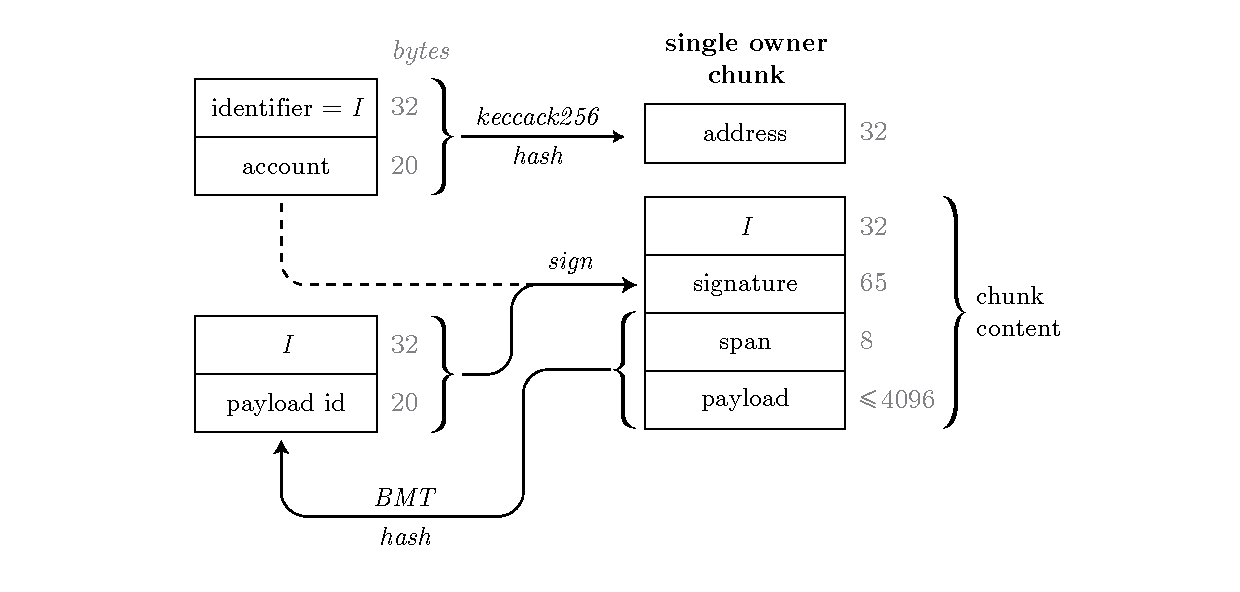
\includegraphics[width=\textwidth]{fig/single-owner-chunk.pdf}
   \caption[Single-owner chunk]{Single-owner chunk. The chunk content is composed of headers followed by the metadata (span) and chunk data of a wrapped content addressed chunk (payload). The first two header fields provide single owner attestation of integrity: an identifier and a signature signing off on the identifier and the content address of the payload. The address is the hash of the id and the signer account.}
   \label{fig:single-owner-chunks}
\end{figure}


The address of a single-owner chunk is calculated as the hash of the owner’s address and an owner-defined identifier. The integrity of single-owner chunk data is warranted by the signature of the owner attesting to the association of arbitrary chunk data with the identifier (see figure \ref{fig:single-owner-chunks}). In other words, each identity owns part of Swarm's address space within which they are free to assign arbitrary content to an address (see definition \ref{def:soc} in appendix \ref{sec:appendix-disc}).



\subsection{Bandwidth incentives and caching of popular content}


Syncing involves transferring chunks from the uploader to storers, i.e., from where they enter the network, to the neighbourhood where the chunk falls within the nodes' \emph{areas of responsibility}. A storer node's role is to serve content by responding to retrieve requests with chunk data.

\begin{figure}[!th]
  \centering 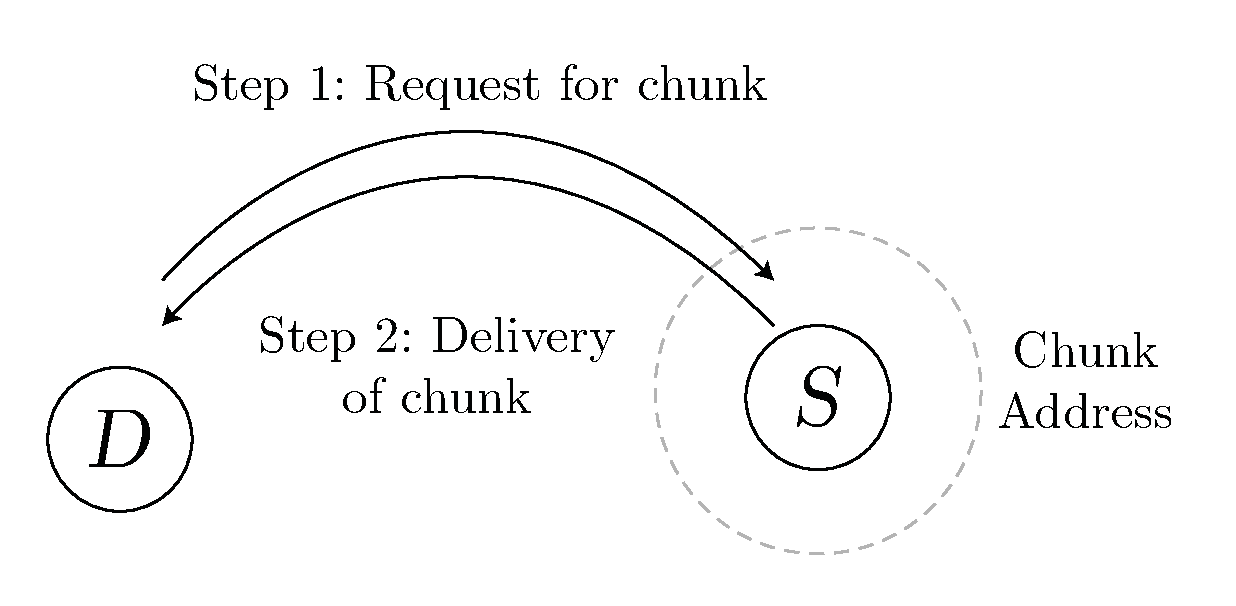
\includegraphics[width=0.5\textwidth]{fig/disc.pdf}
  \caption[DISC]{DISC: Distributed Immutable Store of Chunks. Direct address-based peer-to-peer storage model with forwarding Kademlia routing.}
\label{fig:disc}
\end{figure}


If a node on the way does not have the data itself, it is debited a small amount of BZZ to request chunks from an even closer node. If requests are differently priced based on the expected number of hops needed to route the request, a routing strategy based on selecting the lowest price is expected to mimic a proximity-based one.%
%
\footnote{Nodes also are indirectly motivated to forward the chunk to a node which is closer to the chunk and therefore realise higher forwarding profit. Such "fast forwards" (multiple PO per hop) can be done more often by a node that maintains a larger set of peer connections whose addresses are balanced.}
%
As a consequence of forwarding Kademlia, nodes are also motivated to cache the chunks they serve because, after paying to retrieve the chunk once from a closer node, any subsequent requests for the same chunk will earn pure profit. 

As new content gets added to Swarm, sooner or later, the finite storage capacity of each node will be used up. At this point nodes will need a strategy to decide which chunks should be removed to make way for new chunks. 
The storage cache is pruned regularly when capacity is reached by removing the chunks that were requested the longest time ago. As the recency of the last request is a reasonable predictor of popularity, chunks that generate more income as they are regularly requested will be preferentially retained. Combined with opportunistic caching, this garbage collection strategy both maximises an operator's profit from bandwidth incentives, and, on the network level, ensures that (1) storage capacity is always maximally utilised for increased quality since (2) popular content becomes widely distributed across the network and (3) thus retrieval latency for regularly requested chunks is also decreased.

The closer a node is to the chunk address, the more likely it is that a request for that chunk will end up with them. Therefore, chunks closer to a node's address will be preferentially retained. This creates a weak incentive for storer nodes to sync content. However, it presupposes that the chunk will be the subject of retrieval requests and as such have the promise of some profit. This assumption is not always guaranteed, and is vulnerable to an attack in which an adversary could simply overwhelm the network with chunks that are never requested, and as a result, causing useless chunks to replace useful ones. By attaching a cost to uploading a chunk, Swarm can mitigate such an attack.

\subsection{Rarely accessed content}\label{sec:rarely-accessed-content}

Although effectively providing rewards to storers and forwarders of popular chunks, the flipside of using bandwidth compensation as the only incentive is that chunks that are not accessed for a long time will eventually end up being garbage collected to make room for new arrivals. Therefore, in order for the swarm to be able to guarantee the long-term availability of data, there must be a mechanism with which uploaders can protect their content and prevent their less popular chunks from being prematurely garbage collected.

Moreover, the swarm's incentive system must also ensure that additional revenue is generated for storers of rarely retrieved chunks that would otherwise be deleted. In other words, storers of unpopular chunks that do not generate sufficient profit from retrieval requests only should be compensated for their opportunities forgone. The \emph{postage redistribution} presented in section \ref{sec:redistribution} provides for such compensation: redistribute the revenue resultant of the purchase of \emph{postage stamps} amongst the storer nodes in a fair way.

%%%%%%%%%%%%%%%%%%%%%%%%%%%%%%%%%%%%%%%%%%%%%%%%%%%%%%%%%%%%%%%%%%%%%%%%%%%%%%%%%%%%%%%%%%%%%%%%%%%%%%%
\section{Postage stamps}\label{sec:postage-stamps}

A postage stamp is a verifiable proof of payment associated with a chunk witnessed by the signature of its owner. On the one hand, postage stamps prevent frivolous uploads by imposing an advance cost. On the other hand, by ascribing a quantity of BZZ, they signal a chunk's relative importance which storer nodes can then use to rank chunks when selecting which ones to retain and serve, and which ones to garbage collect in the event of capacity shortage.

In this section we first introduce the concept of postage batch enabling the bulk purchase of stamps (\ref{sec:purchasing-upload}). In \ref{sec:limited-issuance}, we explain how limited issuance is represented and enforced. In \ref{sec:reserve}, we introduce the notion of reserve and detail the rules governing how storer nodes keep it maximally utilised. We conclude in \ref{sec:depths} with exploring the relationship between reserved capacity, effective demand and the number of nodes and their impact on the data availability.

\subsection{Purchasing upload capacity}\label{sec:purchasing-upload}

% \subsubsection{Postage batches and the postage smart contract}

Uploaders purchase postage stamps in bulk in the form of a \emph{postage batch} from the postage smart contract on the Ethereum blockchain. Postage batches are created by this contract when a transaction is sent to its batch creation endpoint, together with an amount of BZZ tokens and transaction data specifying some parameters. As the transaction executes, a new batch entry is registered in the postage contract with the following pieces of information:

\begin{itemize}[noitemsep]
\item[--] \emph{batch identifier} -- A random ID that is generated to provide reference for this batch.
\item[--] \emph{batch depth} -- Base 2 logarithm of the \emph{issuance volume}, i.e., number of chunks that can be stamped using this batch. 
\item[--] \emph{owner address} -- The Ethereum address of the owner entitled to issue stamps, as per the transaction data sent along with the creation or the  transaction sender if not specified.
\item[--] \emph{per-chunk balance} -- The total amount sent along with the transaction divided by the issuance volume.
\item[--] \emph{mutability} -- A boolean flag indicating if the storage slots of the batch can be reassigned to another chunk with a stamp if its timestamp is older. 
\item[--] \emph{uniformity depth} -- the base 2 logarithm of the number of equal-size buckets the storage slots are arranged in.
\end{itemize}

The postage contract provides endpoints to users to modify the per-chunk balance of batches, i.e., add funds to extend the validity period of the stamps issued by the batch (\/\emph{top-up}) or add volume to decrease it (\/\emph{dilute}).
Anyone can then choose to top up the balance of a batch at a later date but only the owner can dilute it.%
%
\footnote{As a planned feature, the remaining balance of a batch can be reassigned to a new batch, resulting in the immediate expiry of the original.}


% \subsubsection{Stamp validity}

\begin{figure}[!ht]
  \centering
    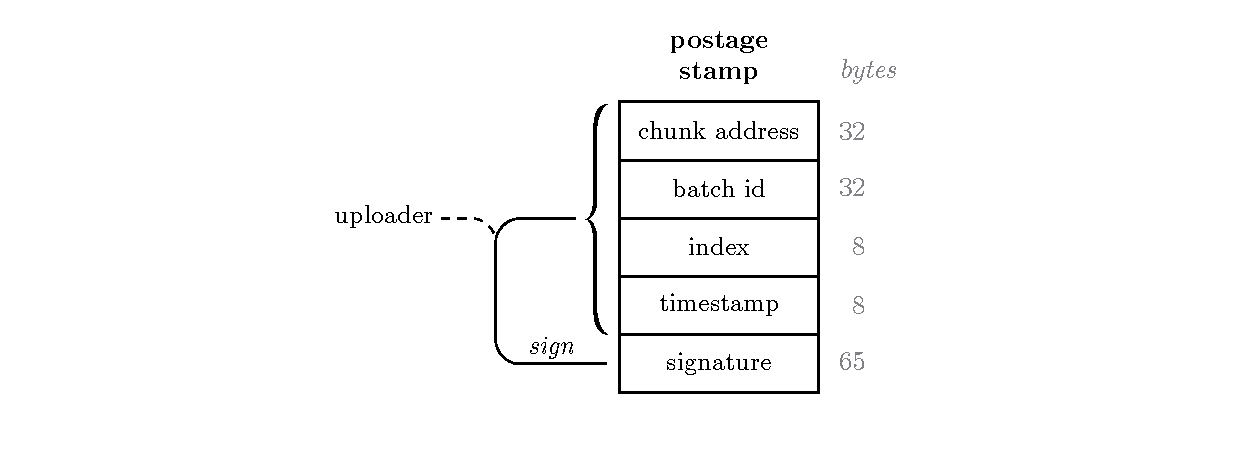
\includegraphics[width=\textwidth]{fig/postage-stamp-structure.pdf}
  \caption[Postage stamp]{Postage stamp is a data structure comprised of the postage contract batch id, storage slot index, timestamp the chunk address and a witness signature attesting to the association of these four. Uploaders and forwarders must attach a valid postage stamp to every chunk uploaded. }
  \label{fig:postage-stamp}
\end{figure}

Owners issue postage stamps in order to attach them to chunks (see definition \ref{def:postage-stamp} in appendix \ref{sec:appendix-disc}). A batch has a number of \emph{storage slots} effectively arranged over a number of equal sized buckets. Issuing a stamp means to assign a chunk to a storage slot. A stamp is a data structure comprising the following fields (see figure  \ref{fig:postage-stamp}):

\begin{itemize}[noitemsep]
    \item[--] \emph{chunk address} -- The address of the chunk the stamp is attached to. 
    \item[--] \emph{batch identifier} --  The ID referencing the issuing batch (generated at its creation).
    \item[--] \emph{storage slot} -- An bucket index referencing one of the equal sized buckets of the batch and a within-bucket index referencing the storage slot the chunk is assigned to.
    \item[--] \emph{timestamp} -- The time the chunk is stamped. 
    \item[--] \emph{witness} -- The batch owner's signature attesting to link between the storage slot and the chunk.
\end{itemize}

A postage stamp's validity can be checked by verifying that it scores all true on the following five attributes (see definition \ref{def:postage-stamp-validity} in appendix \ref{sec:appendix-disc}):

\begin{itemize}[noitemsep]
\item[--] \emph{authentic} -- The batch identifier is registered in the postage contract's storage.
\item[--] \emph{alive} -- The referenced batch has not yet exhausted its balance.
\item[--] \emph{authorised} -- The postage stamp is signed by the address specified as the owner of the batch. 
\item[--] \emph{available} -- The referenced storage slot is within range given the batch depth, and, in the case of an immutable batch, has no duplicates.
\item[--] \emph{aligned} -- The referenced storage slot has the bucket specified and it aligns with the chunk address stamped.
\end{itemize}

All this can be easily checked by nodes in the swarm only using information available on the public blockchain (read-only endpoints of the postage contract). When a chunk is uploaded, the validity of attached postage stamp is verified by forwarders along the push-syncing route  (see figure \ref{fig:postage-stamps}).


\begin{figure}[!th]
\centering
  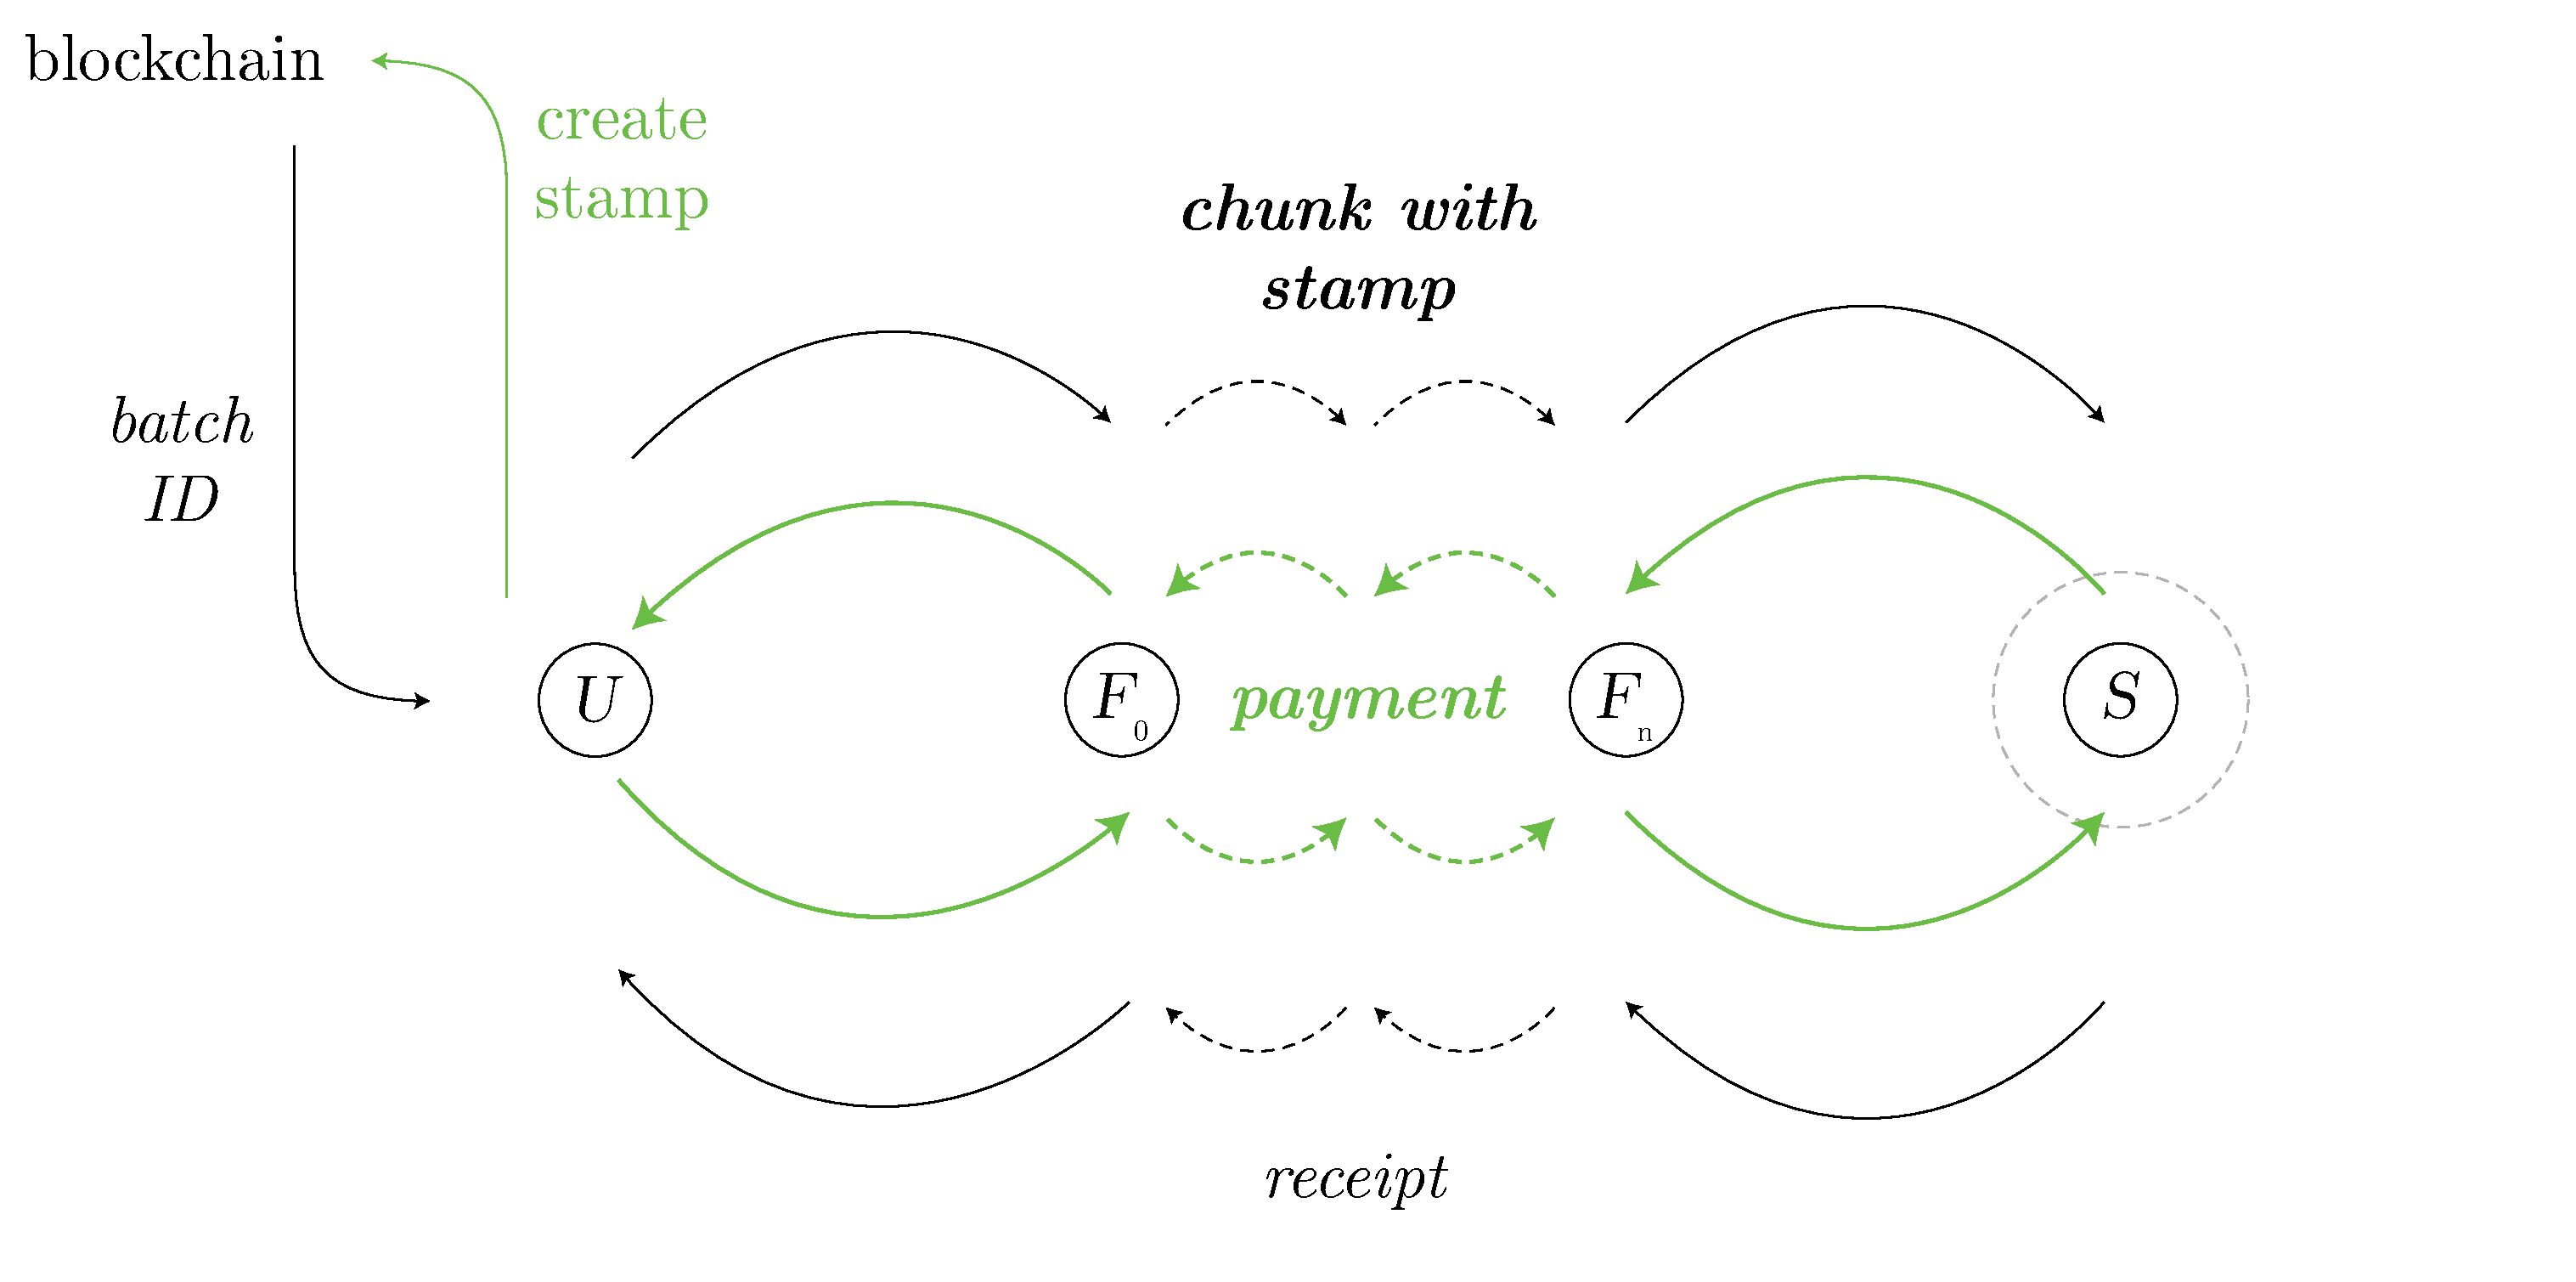
\includegraphics[width=\textwidth]{fig/postage-stamp.pdf}
\caption[Postage stamps]{Postage stamps are purchased in bulk on the blockchain and attached to chunks at upload. They are passed along the push-syncing route together and their validity is checked by forwarders at each hop. }
\label{fig:postage-stamps}
\end{figure}

The normalised per-chunk balance of a batch is calculated as the batch inpayment divided by the batch size in chunk storage slots. The chunk balance is interpreted as an amount pre-committed to be spent on storage. The balance decreases with time as if \emph{storage rent} was paid for each block at the price dictated by the price oracle contract.  

This system allows prepayment for storage without having to speculate on the future price of storage or fluctuations in the currency's exchange rate. At the cost of decreased certainty about the expiration date, one gains resilience against price volatility. On top of this, uploaders can enjoy the luxury of non-engagement by tying up more of the batch balance; while it serves as collateral against price increase, if that does not happen the funds can still be used up (for storing).


\subsection{Limited issuance}\label{sec:limited-issuance}

% \subsubsection{Issuing postage stamps}

Purchasing a postage batch effectively entitles the owner to issue a fixed amount of postage stamps against the batch ID called the \emph{issuance volume} or \emph{batch size}. It is restricted to the powers of 2 and is specified using the base 2 logarithm of the amount which is called \emph{batch depth}. Storage slots of a batch are arranged in a number of buckets and are indexed within the bucket. The number of buckets is restricted to the powers of 2 and is specified using its base 2 logarithm called \emph{uniformity depth}. The size limitation of a batch with batch depth $d$ and uniformity depth $u$ is equivalent to the conditions that 1) the bucket index ranges from 0 to $2^u-1$, 2) the within-bucket index ranges  from 0 to $2^{d-u}-1$ and 3) there are no duplicate indexes.  

While 1) and 2) is easily verifyable by any third party, 3) is not.
In order for index collisions to be detectable by individual storer nodes, uniformity depth must be large enough to fall within nodes' area of responsibility.
As long as this is maintained, all chunks in the same bucket are guaranteed to land in the same neighbourhood, and, as a result, duplicate assignments can be locally detected by nodes (see figure \ref{fig:over-issuance}).

In order to keep their stamps collision-free, uploaders need to maintain counters for how many stamps they have issued for each bucket of a batch and must not issue more than the allowed bucket size. 

\begin{figure}[!ht]
  \centering
    
\includegraphics[width=1\textwidth]{fig/batch-structure.pdf}
  \caption[Batch structure, uniformity and over-issuance]{Batches come with $2^u$ equal-sized buckets ($u$ is uniformity depth, orange circle) each containing an equal number of storage slots ($2^{d-u}$) adding up to batch capacity of $2^d$ chunks ($d$ is batch depth, red circle). Storage slots are indexed and the index is associated with a chunk via the stamp signature. Postage stamp over-issuance is detected locally by storer nodes as long as the buckets are deeper than their storage depth (green circle), as in the diagram on the left. In this case they will receive all the chunks that are correctly assigned to the relevant bucket (orange radii) and correctly identify collisions (red radii) by forbidding indexes that are either out of range ($\geq 2^{d-u}$) or multiply assigned. In contrast, the diagram on the right shows it is not possible for a node with storage depth 4 to identify duplicates for a batch with $u=2$}
\label{fig:over-issuance}
\end{figure}    



In general, the most efficient utilisation of a batch is by filling each bucket fully.%
%
\footnote{See appendix \ref{sec:batch-utilisation} for a detailed analysis of batch utilisation.
% \subsubsection{Efficiency of batch utilisation}
}
%       
Continued non-uniformity (i.e., \emph{targeted issuance}) leads to underutilised batches, and therefore a higher unit price for uploading and storing each chunk. This feature has the desired side effect that it imposes an upfront cost to non-uniform uploads: the more concentrated the distribution of chunks of an upload, the more storage slots of the postage batch remain unused. In this way, we ensure that targeted denial-of-service attacks against a neighbourhood (i.e., uploading a disproportionate number of chunks in a particular address range) is costly since the \emph{inert cost} (due to the degree of under-utilisation of the batch) is exponential in the depth of the skew.

Beyond DoS protection, postage stamps can serve as a \emph{fiduciary signal} indicating how much it is worth for a user to persist a chunk in Swarm. In particular, the per-chunk balance of batches can provide the differential a priori bias determining which chunks should be protected from garbage collection in the absence of evidence to predict their profitability from swap. 



\subsection{Rules of the reserve}\label{sec:reserve}

% \subsubsection{Batch balance, rent and expiry}\label{sec:rent-expiry}

The \emph{reserve} is a fixed size of storage space dedicated to storing the chunks in the node's \emph{area of responsibility}. Chunks in the reserve are the chunks that are protected against garbage collection with valid postage stamps. When batches expire, i.e., their balance is completely depleted, the chunks they stamped are no longer protected from eviction. Their eviction from the reserve frees up some space that can accommodate new or farther chunks belonging to valid batches.


From the point of view of incentives, chunks which are of the same proximity order and the same batch are equivalent. When it comes to eviction due to batch expiry, these equivalence classes, called \emph{batch bins} are handled as one unit: the chunks in a batch bin are evicted from the reserve and inserted to the cache in one atomic operation. 

Assuming a global oracle for the unit price of rent and a fixed reserve capacity  prescribed for nodes, the content of the reserve is coordinated with  a set of constraints on batch bins called the \emph{rules of the reserve}:
\begin{itemize}[noitemsep]
    \item[--] if a batch bin of a certain PO is reserved then the batch bins are reserved also for all closer bins (higher PO). 
    \item[--] if a batch bin is reserved at a certain proximity order (PO), then all the batch bins at the same PO belonging to batches with a greater per-chunk balance are also reserved. 
    \item[--] the reserve should not exceed capacity.
    \item[--] the reserve is maximally utilised, i.e, cannot be extended and have 1-3 remain true.
\end{itemize}

The first rule means the reserve is closed upwards for PO, which encodes a global preference for  chunks closer to the node's address. This is incentivised by routing: keeping the closest chunks, a node will maximise the number of receipts it can issue and the number of retrieve requests it can respond to and at the same time provides the widest coverage within the neighbourhood even after the neighbourhood is no longer supporting the desired redundancy.

The second rule expresses the constraint that the reserve for a PO is upward closed for per-chunk balance, which encodes a secondary preference among chunks of the same proximity for those stamped using a batch with higher per-chunk balance. This is incentivised by the differential absolute profit chunks promise: due to the  constraint that balances are not revocable, chunks with higher balance expire later and therefore contribute more to storers' absolute profit than those expiring earlier despite the same rent paid during their period of validity.%
%
\footnote{Note that even if there was no scheme for redistributing postage revenue and the inpayments are frozen/burnt, this strategy is still mildly incentivised in as much as it is aligned with token-holders interest: batches with higher balance exert more deflationary force on the token (per chunk, i.e, the unit of invested resource) by keeping their balance frozen which is expected to realise in a proportional price increase.}


\begin{figure}[!ht]
  \centering
    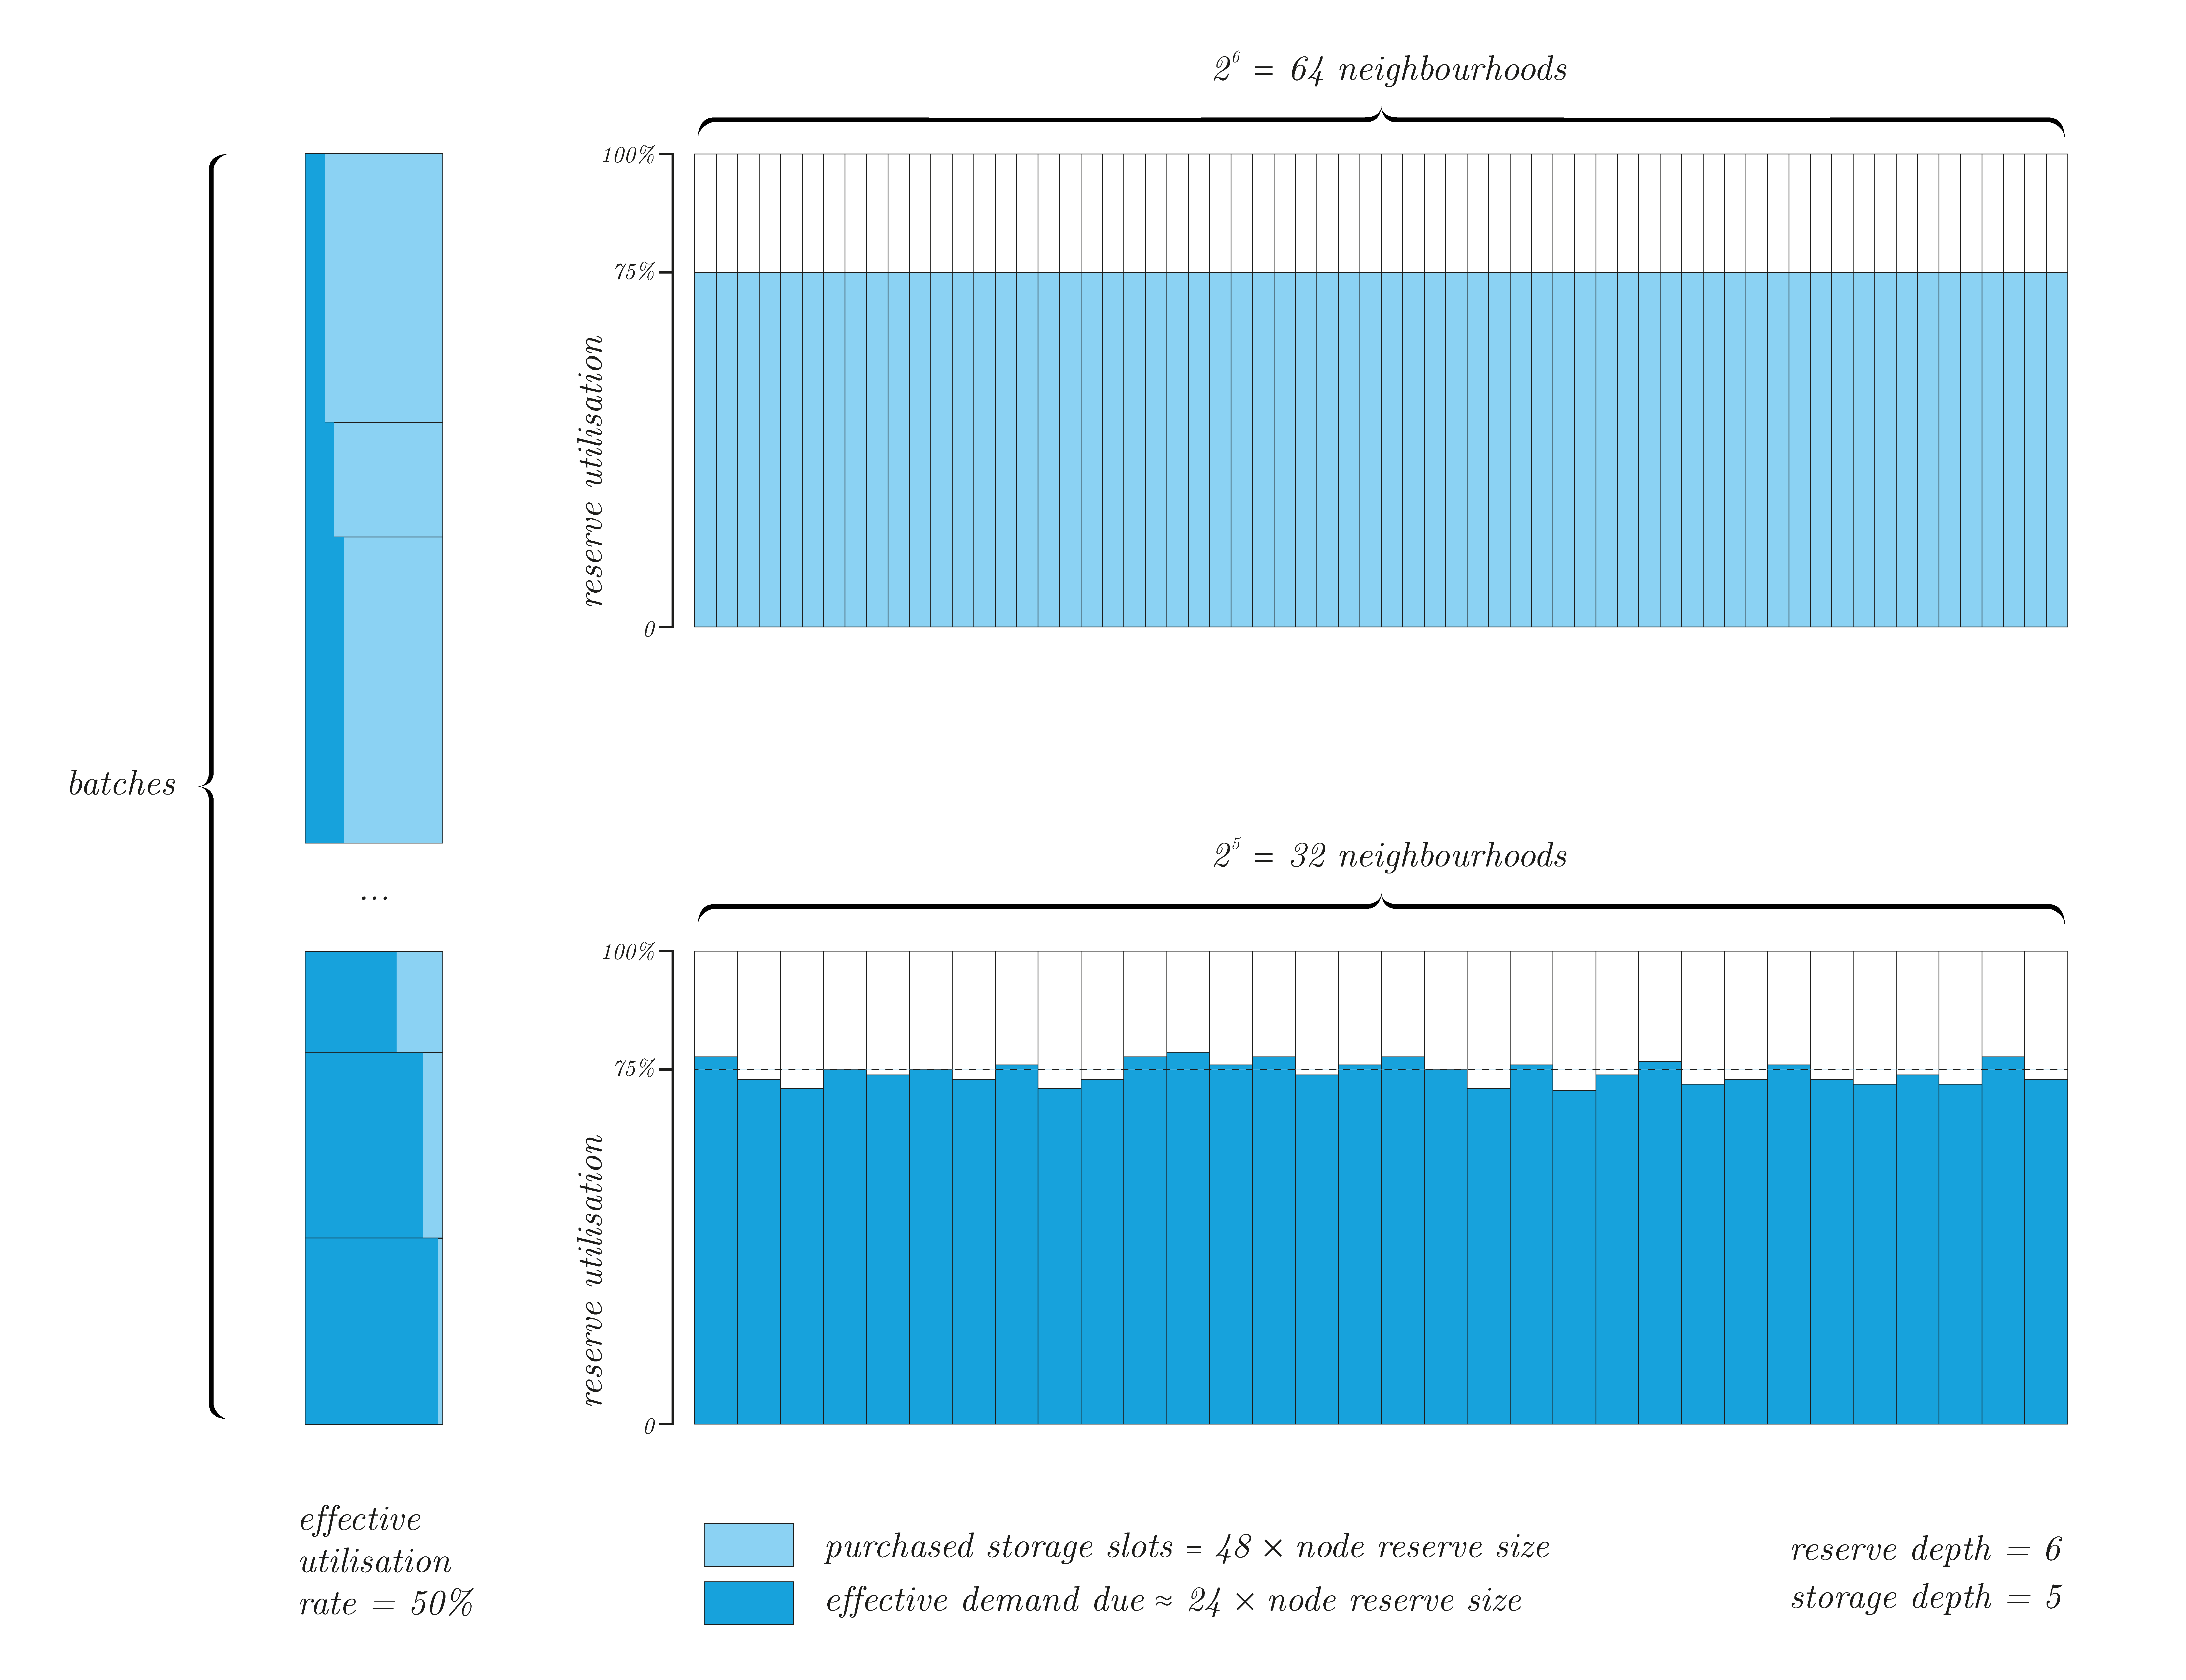
\includegraphics[width=.9\textwidth]{fig/supply-demand.pdf}
  \caption[Reserve capacity]{Potential demand for chunk storage is expressed by the total size of all batches with non-zero balance on the blockchain (left). The lower bound on neighbourhood depth to store this capacity is the reserve depth (top right). Storage depth marks the effective volume of chunks uploaded and stored in a neighbourhood's reserve (bottom right). The difference between them is a result of partial batch utilisation. The uniformity of the volume of chunks across neighbourhoods is incentivised by the efficient utilisation of postage batches.}
\label{fig:reserve-capacity}
\end{figure}    

When a new chunk arrives in swarm through pull-sync, push-sync or upload, the validity  of the attached  postage stamp is verified. If the PO of the chunk is lower than the batch depth, the node inserts the chunk into the  garbage collection index, otherwise it is by definition in the reserve. 
If the reserve size is above capacity, a number of batch bins are identified so that their total size covers the excess so that after these batch bins are \emph{evicted} from the reserve, the reserve size will be within capacity. 


\subsection{Reserve depth, storage depth, neighbourhood depth}\label{sec:depths}



\subsubsection{Reserve depth}

The potential demand for chunks to be stored in the DISC is quantified by the total storage slots of valid batches. This is calculated as the sum of the sizes of non-expired batches. Since the batches and their balances are recorded in the postage contract, the reserved DISC size is under consensus.%
%
\footnote{The volume is best explicitly maintained by the contract by adding the size of newly created batches and deduct the sizes of newly expired batches. DISC reserve size is updated each time a batch is created or topped up and expired batches are removed during each redistribution round, executed as part of the process triggered by the claim transaction.}  

The base 2 logarithm of the DISC reserve size rounded up to the nearest integer is called the \emph{reserve depth}. The reserve depth is the shallowest PO such that disjoint neighbourhoods of this depth are collectively able to accommodate the volume of data corresponding to the total number of chunks paid for, assuming that nodes in the neighbourhood have a fixed prescribed storage capacity to store their share of the reserve. 

The reserve depth is also the \emph{safe lower bound} for pull-syncing, i.e, the farthest bin a neighbourhood needs to synchronise to guarantee storing the reserve.
Conversely, if any neighbourhood marked by reserve depth has no nodes in it, the swarm is not working correctly, i.e., chunks with valid stamps are not protected from getting lost. See figure \ref{fig:depths}.

\subsubsection{Storage depth}

The \emph{effective demand} for chunks to be stored in the DISC is the total number of chunks actually uploaded. While each chunk in the reserve has a valid postage batch and therefore is assigned to a storage slot, a postage batch can always have some of its storage slots unassigned. This entails that the number of chunks actually stored in the DISC can in fact be a fraction of the DISC reserve size. 

The effective area of responsibility is  marked by the proximity order of the farthest batch bin of the reserve assuming the node complies with the rules of the reserve. 

A node's \emph{storage depth} is defined as the shallowest \emph{complete} bin, i.e., the lowest PO that compliant reserves stores all batch bins at. Unless the farthest bin in the node's reserve is complete, the storage depth equals the reserve's edge PO plus one.

The storage depth is the \emph{optimal lower bound} for pull-syncing, i.e, the farthest bin the node needs to synchronise with its neighbours to achieve maximum reserve   utilisation.%
%
\footnote{The nodes will have full connectivity upto the shallowest bin that they are pull syncing. This choice is incentivised by the risk of having two disjoint connected sets of pull-syncing nodes resulting in non-consensual reserve. As a consequence, we can say that storage depth is an upper bound on the depth of full connectivity.}
%
Maximum reserve utilisation should be incentivised as part of the storage incentives. 

% See figure \ref{fig:reserve-depth-vs-storage-depth}.

% \begin{figure}[!ht]
%   \centering
%     % \includegraphics[width=\textwidth]{fig/reserve-depth-vs-storage-depth.pdf}
%   \caption[Reserve depth vs storage depth]{Reserve depth vs storage depth.}
% \label{fig:reserve-depth-vs-storage-depth}
% \end{figure}    




% \subsubsection{Batch utilisation rate}\label{sec:utilisation-rate}

The gap between actual storage depth and the  reserve depth exists because of the bulk purchase of stamps. Since entire batches of stamps reserve storage slots that are assigned to  chunks only at later times when they are actually uploaded, the batch \emph{utilisation rate} can be substantially less than 1 (see appendix \ref{sec:batch-utilisation}). Storage depth and reserve depth are the same only if all batches are fully utilised. 


\subsubsection{Neighbourhood depth}

Swarm's requirements on local replication is that each neighbourhood designated by the storage depth contains at least four nodes. 
If neighbourhoods were made of one node, then the outage of that one node will make  the chunks in the node's area of responsibility not retrievable.
With two nodes in a neighbourhood, we significantly improve resilience against ad-hoc outages, but because of connectivity latencies a two-peer neighbourhood still displays unstable user experience.
The ideal scenario is to have four nodes per full connectivity neighbourhood, which prompts the following definition: \emph{neighbourhood depth} for a particular node is the highest PO $d$ such that the address range designated by the $d$-bit-long prefix of the node's overlay contains at least 3 other peers.


Figure \ref{fig:depths} details the potential relative orders of the three depths and their consequences on the health, efficiency and redundancy of the swarm.

\begin{figure}[!ht]
  \centering
    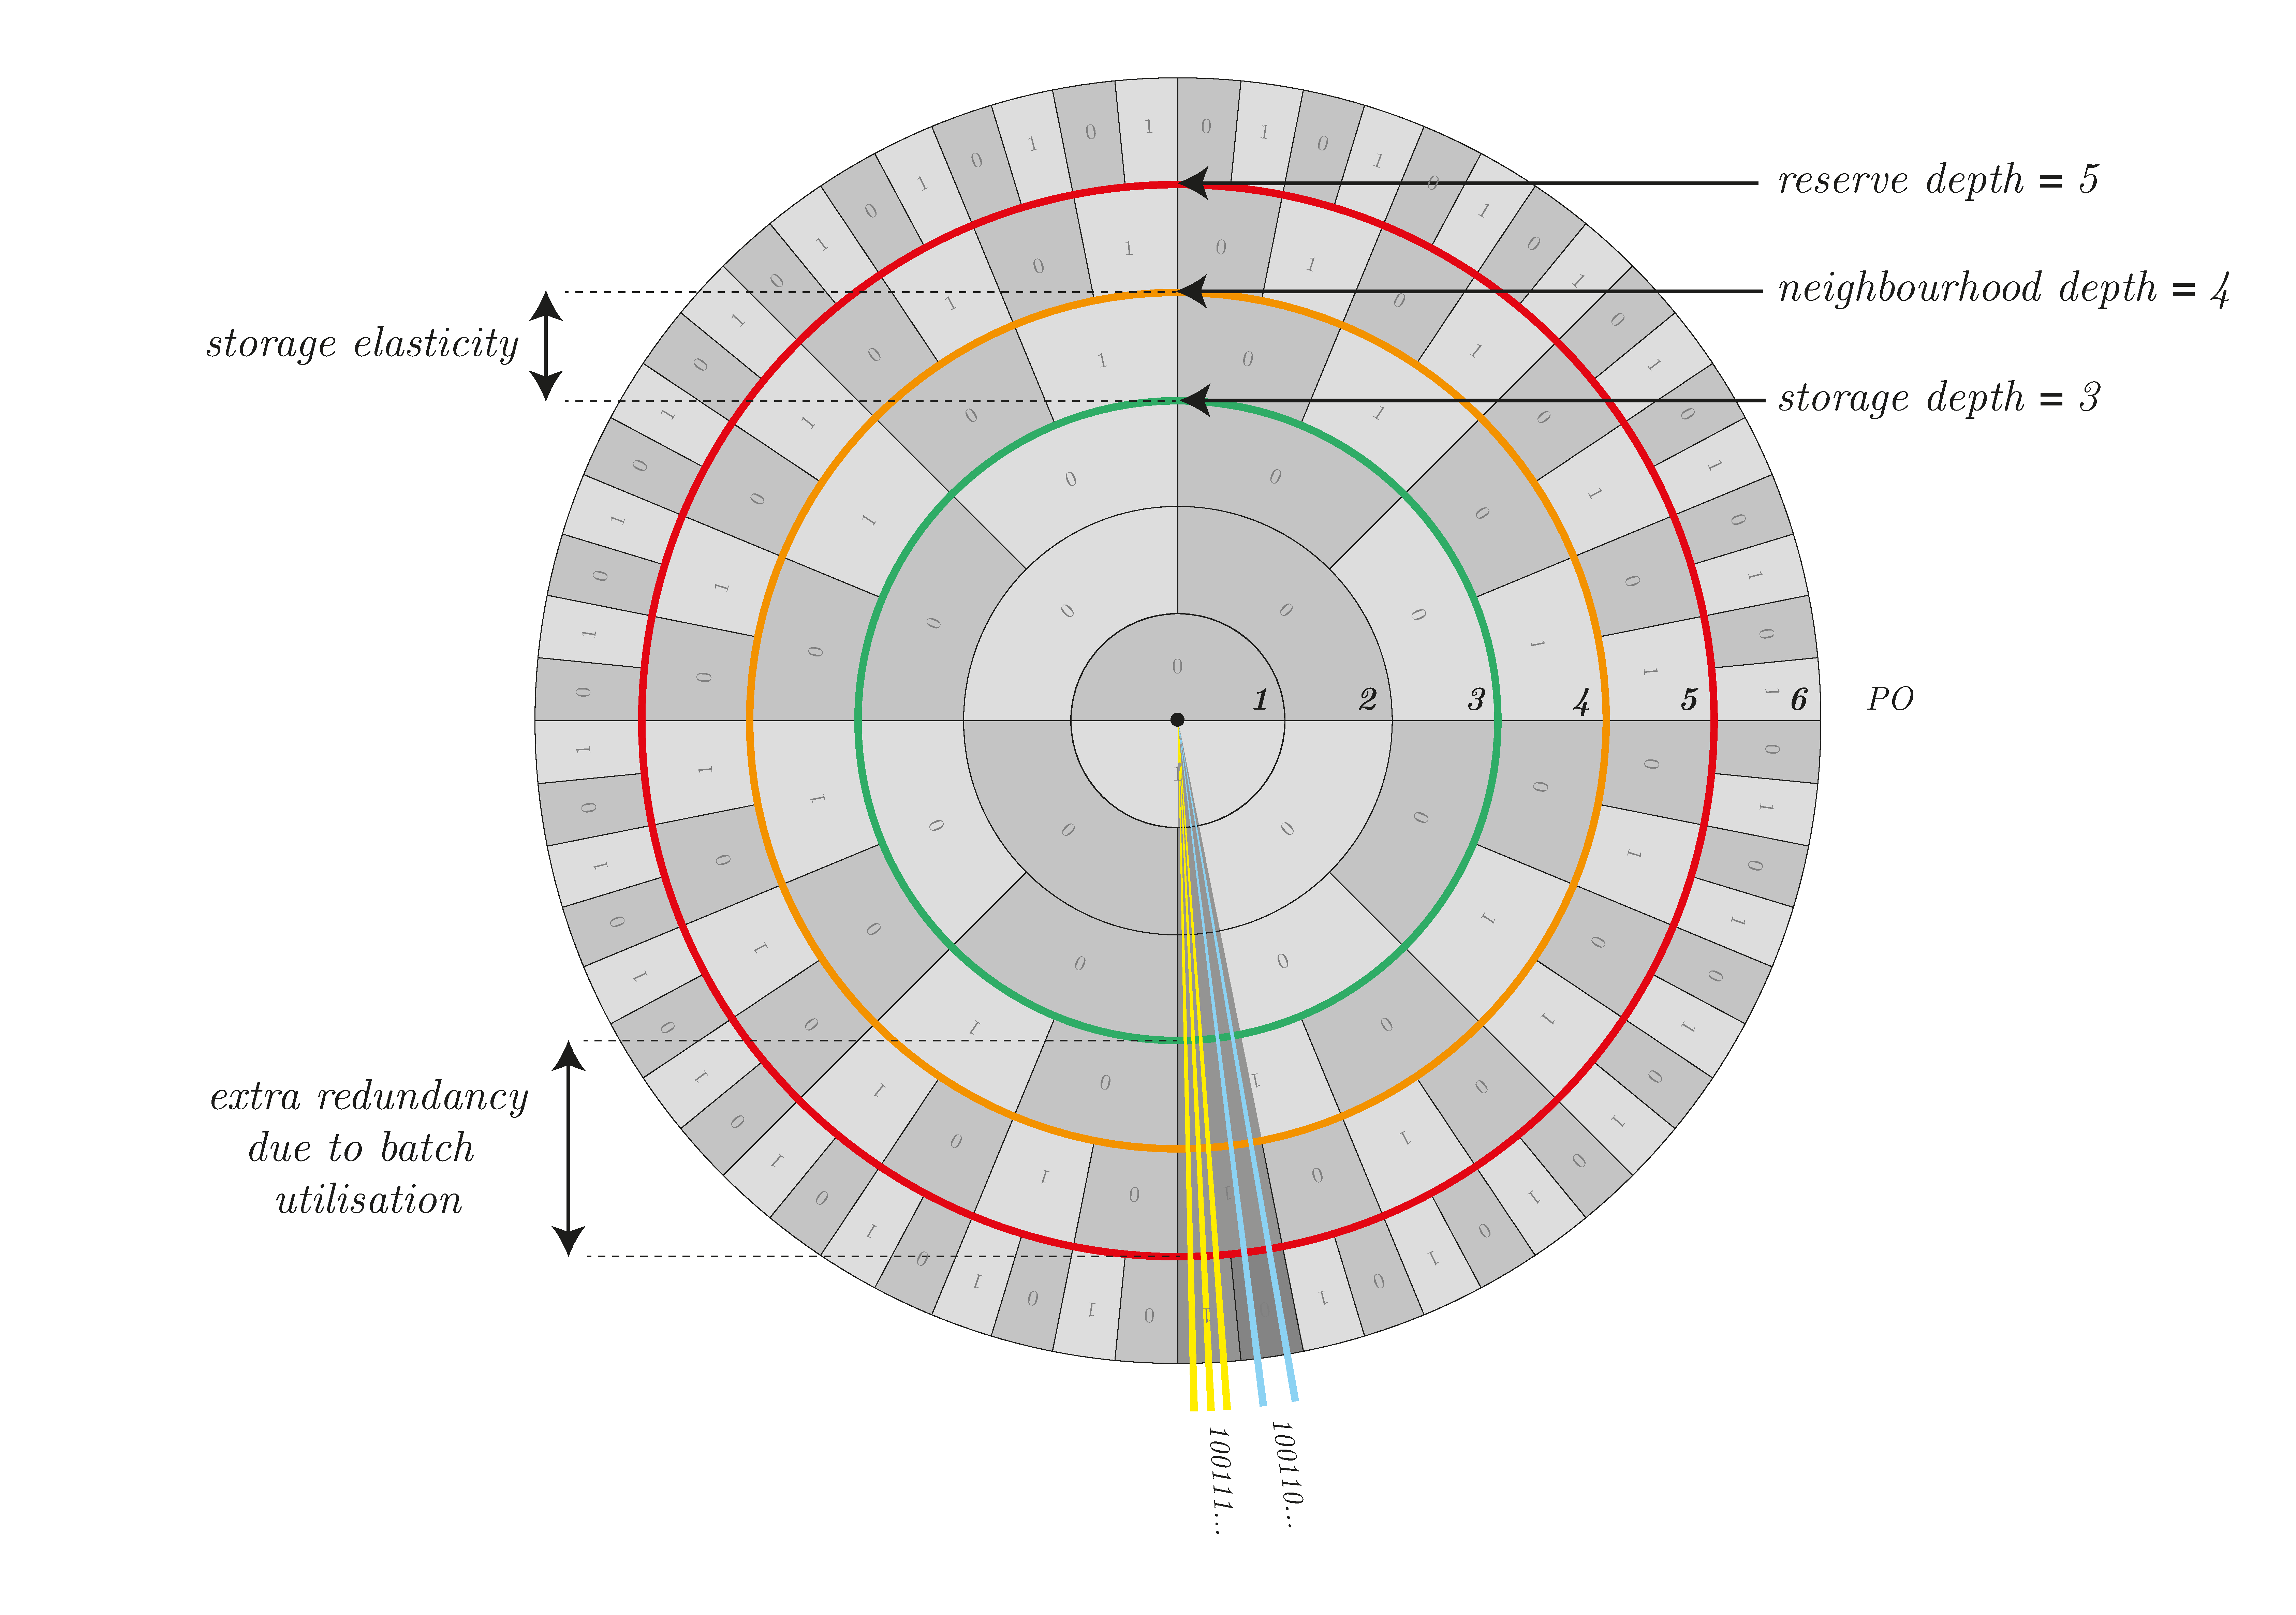
\includegraphics[width=.7\textwidth]{fig/depths-2.pdf}
  \caption[Depths]{The 3 depths (reserve, storage and neighbourhood) express the order of magnitude of reserved capacity (potential demand, red circle), uploaded chunks (effective demand, green circle) and the number of nodes (effective supply, orange circle), respectively. Their possible orderings express different scenarios with characteristic impact on data availability. Storage depth cannot be greater than reserve depth. A gap between storage depth and reserve depth quantifies the average batch utilisation rate. The gap between storage depth and a deeper neighbourhood depth quantifies the elasticity of the storage: the difference expresses how many times the effective volume can double before redundancy goes below required. While such oversupply may be anticipatory of growth in demand, if neighbourhood depth remains deeper than storage depth long term, it may indicate excessive profits. The opposite order indicates undersupply (redundancy below the desired level).}
\label{fig:depths}
\end{figure}    
%%%%%%%%%%%%%%%%%%%%%%%%%%%%%%%

% In the introduction we concluded that Swarm needs to have a subsystem for users to signal the importance/relevance of chunks. Postage stamps (and batches) were presented as a framework to implement storage incentives to ensure rarely accessed content remains available. 

%%%%%%%%%%%%%%%%%%%%%%%%%%%%%%%%%%%%%%%%%%%%%%%%%%%%%%%
\section{Fair redistribution}\label{sec:redistribution}


The system of positive%
%
\footnote{The concept of \emph{positive incentives} refers to a scheme whereby providers of a service are entitled to reward but there is no loss involved if they discontinue their service or are not online.}
%
storage incentives in Swarm is concerned with redistributing  to storage providers the BZZ tokens that uploaders deposited within the postage contract.%
%
\footnote{As explained earlier, uploaders pay in an unwithdrawable amount to the postage contract which serves as the balance to pay storage rent. In exchange they obtain the right to issue a fixed number of postage stamps which they attach to chunks they want the network to store.}
%
The overall balance on the contract covers the \emph{reward pot} which represents the total \emph{storage rent} cumulated over all postage batches for a particular period. The storage rent must be redistributed to storage providers in a way that guarantees that their earnings are proportional to their contribution weighing in storage space, quality of service and length of commitment.

The procedure for redistribution is best conceived of as a game orchestrated by a suite of smart contracts on the blockchain. Nodes earn the right to play through participation in storing and syncing chunks.  
The winners claim their reward by sending a transaction to the game contract. 

In section \ref{sec:uniformity-pot}, we formulate the idea of redistribution in terms of probabilistic outpayments to allow an easy proof of fairness. Next, in \ref{sec:mechanics}, we introduce the mechanics of the redistribution game.
Then, in \ref{sec:staking} and \ref{sec:por} we explain how we enforce maximum utilisation of dedicated storage for persisting  relevant content redundantly. We conclude in \ref{sec:price-oracle} by discussing how to read certain aspects of the game as price signals that render the network self-regulating through automatic price discovery. 

\subsection{Neighbourhoods, uniformity and probabilistic outpayments}\label{sec:uniformity-pot} 

In this section we argue that the efficient use of postage batches incentivises a balanced chunk distribution which in turn gives rise to uniform storage depth across neighbourhoods. We then explain how this enables a fair system of redistribution using probabilistic outpayments.
% \subsubsection{Uniformity}


Assuming an oracle that sets the unit price of storage, the storage rent due for a period of time for a batch can be calculated. The number of rent units for a batch is the result of multiplying the size of the batch with the number of blocks in the period. The price of rent is calculated from the number of rent units multiplied by the unit price.%
%
\footnote{If this theoretical amount is less than the the current balance of the batch, then the batch is expired and the effective rent is only the remaining balance.}
%
The total storage rent cumulated over all batches for the period between two outpayments constitutes the \emph{reward pot} for the round.

Instead of dividing the reward pot among neighbourhoods regularly, the entire reward pot can be transferred to (representative nodes in) one target neighbourhood in each round. This probabilistic outpayment scheme is fair on the level of neighbourhoods as long as we can make sure that over a large number of rounds the probability with which a  
neighbourhood is selected as the target corresponds to its relative contribution to the overall network storage. Given a constant prescribed reserve capacity and replication of the reserve content by nodes in a neighbourhood, each neighbourhood defined by storage depth contributes equally to the network. 

In section \ref{sec:postage-stamps}, we wrote that uploaders are strongly incentivised to use their postage batch in a way that the chunks they stamp with it are uniformly distributed across the address space. This being true of all batches creates a situation that chunks are uniformly distributed across the DISC. In particular, the sets of chunks sharing a prefix are expected to be roughly equal in size. Therefore we expect nodes to fill their prescribed reserve capacity with chunks at the same proximity order, irrespective of their location in the address space, i.e., the storage depth is uniform across  nodes and therefore across neighbourhoods.%
%
\footnote{Differences do occur due to variance but over many rounds, deviation from the mean is meant to be independent of the location.}
%
With neighbourhoods at equal depth, uniform sampling of neighbourhoods can be modelled by choosing the neighbourhood which contains an anchor (called the \emph{the neighbourhood selection anchor}%
%
\footnote{one of the random nonces (see definition \ref{def:nonce-round}) from the \emph{random seed} of the round, see appendix \ref{sec:randomness}.}
%
) randomly dropped in the address space (see figure \ref{fig:neighbourhood-selection}).


\begin{figure}[!ht]
  \centering
    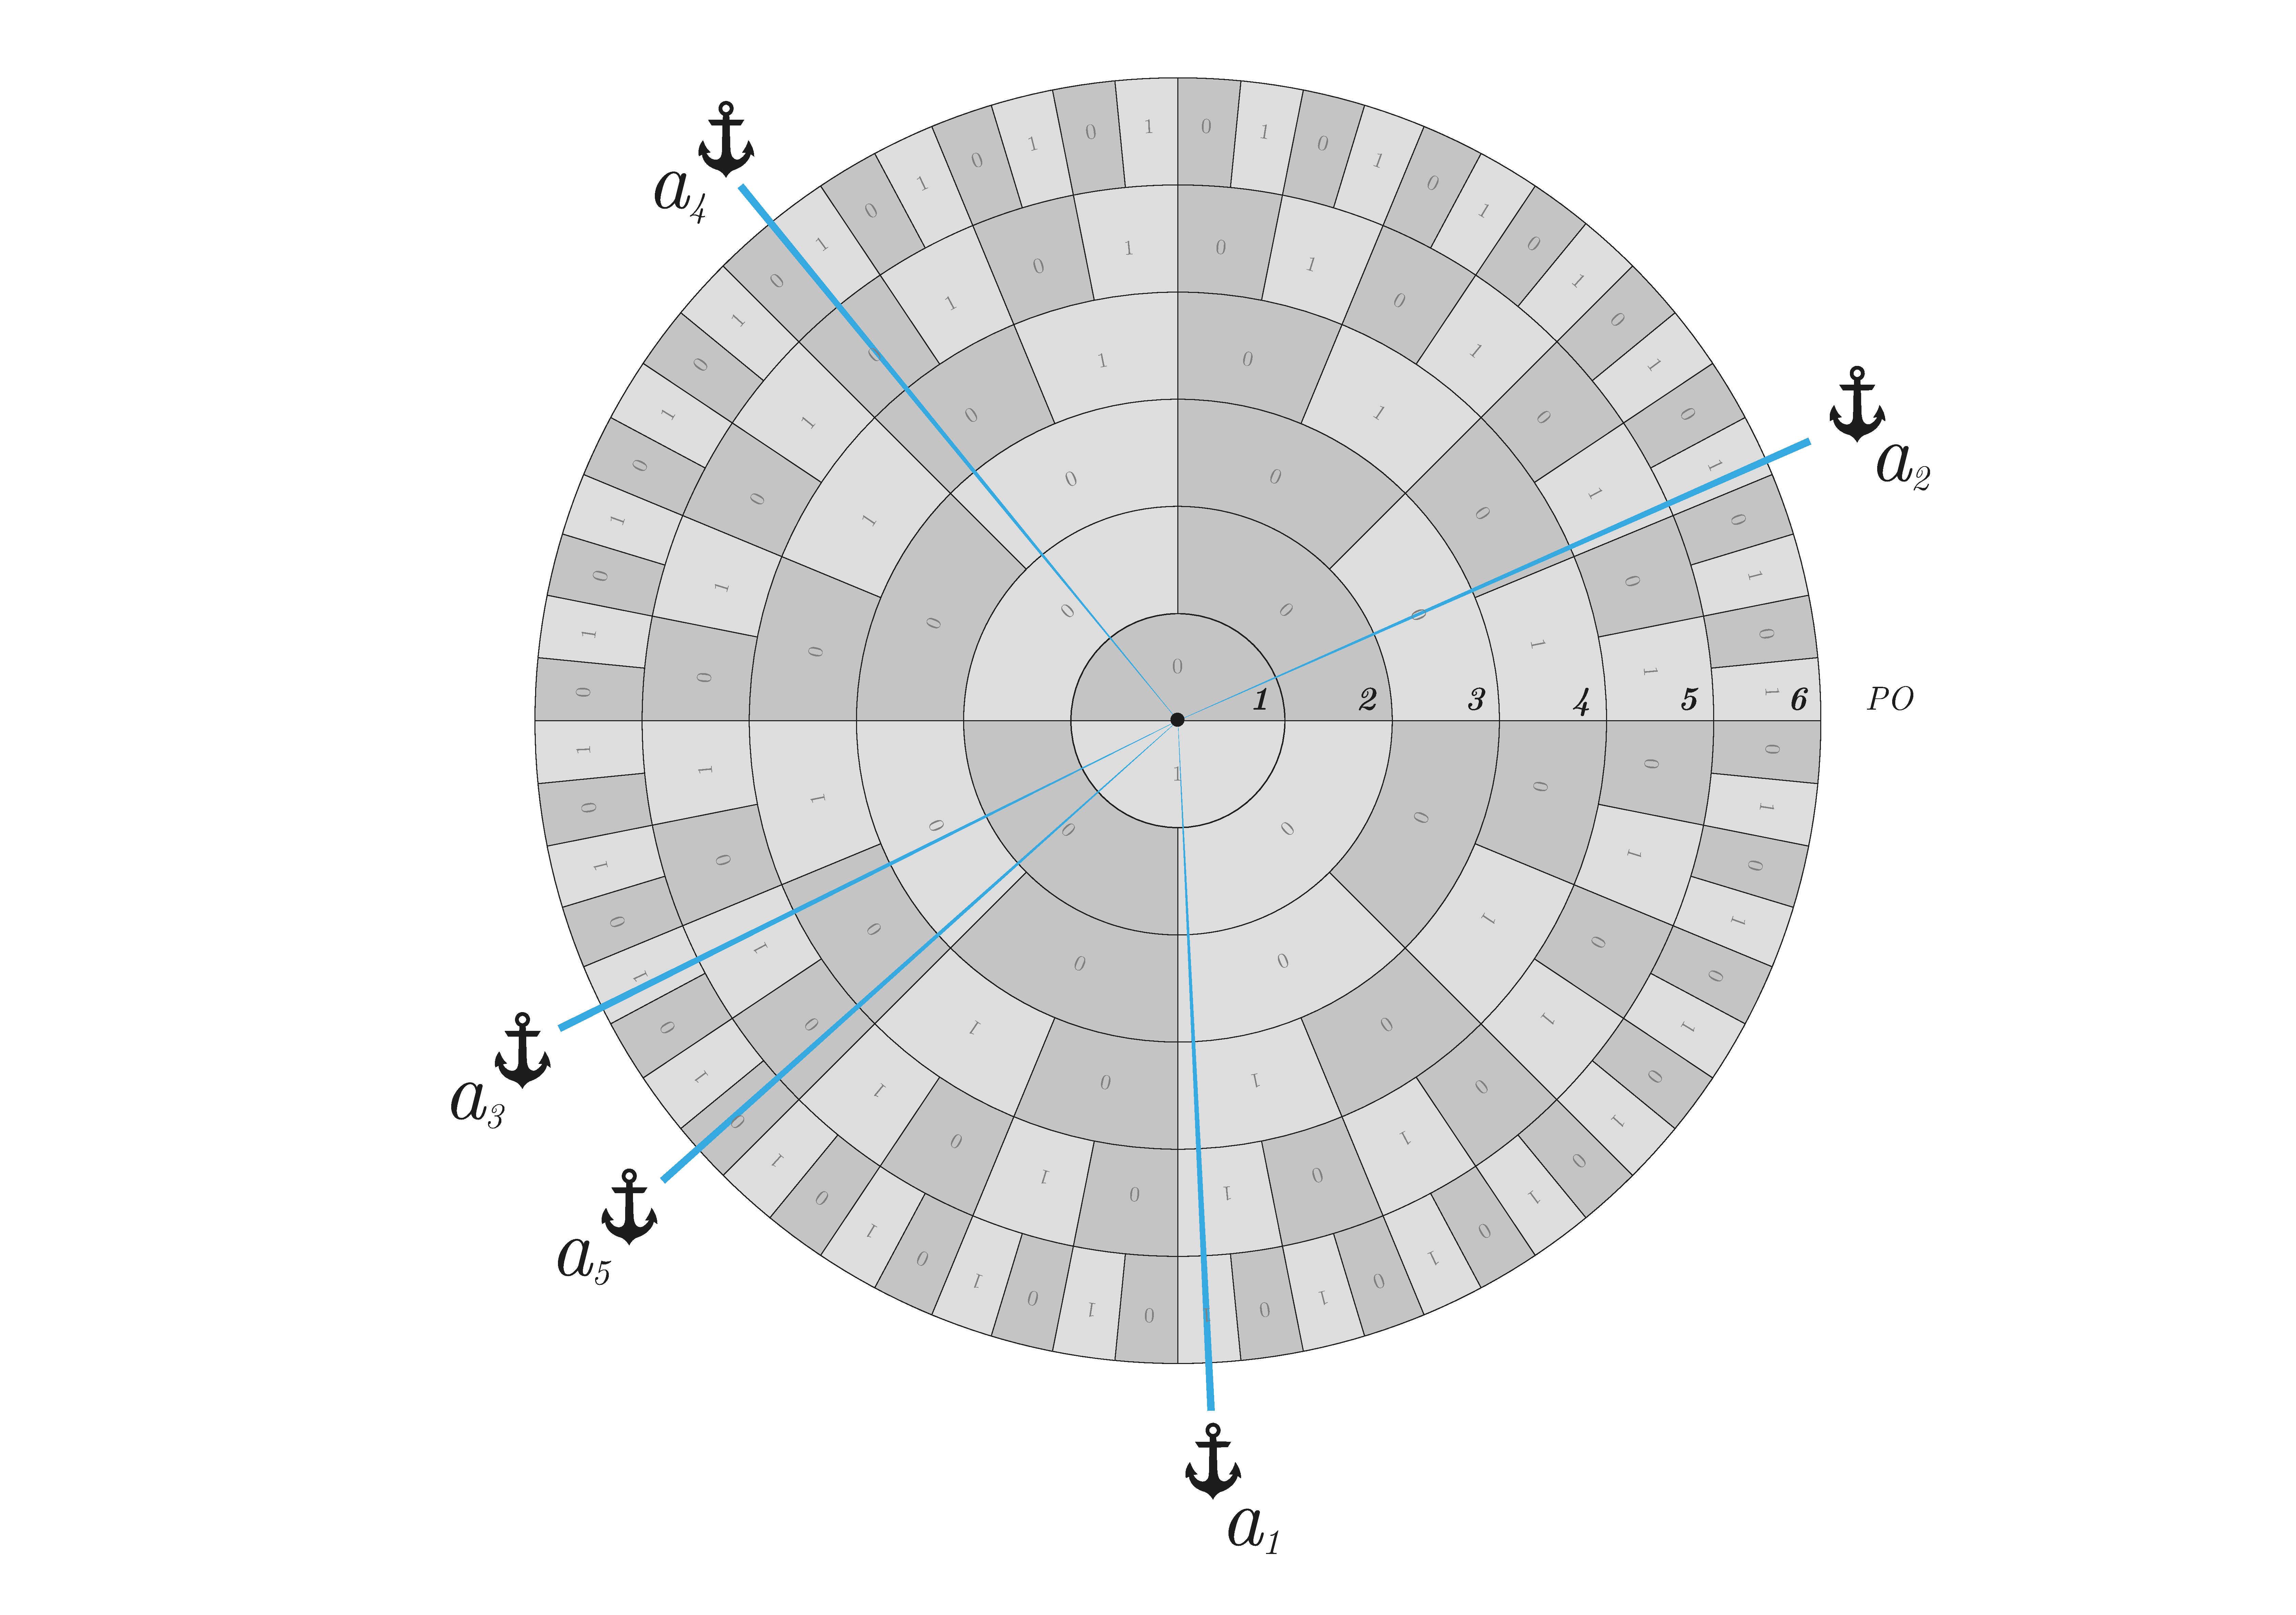
\includegraphics[width=\textwidth]{fig/nhd-selection.pdf.pdf    }
  \caption[Neighbourhood selection and pot redistribution]{Neighbourhood selection and pot redistribution. The winning locality is selected by the neighbourhood selection anchor. Neighbourhoods that contain the anchor within their storage depth are invited to submit an application by committing to a consensual reserve sample. }
\label{fig:neighbourhood-selection}
\end{figure}    

    


\subsection{The mechanics of the redistribution game}\label{sec:mechanics}

The cooperation of peers to redundantly store for the network's benefit is underpinned by a \emph{Schelling game} (defined formally in appendix \ref{sec:redistribution-game}) aimed at proving that the peers agree on the chunks they need to store and they do, in fact, store them. The redistribution game itself is orchestrated by the game contract, one of the building blocks of the system of 4 smart contracts which collectively drive the swarm storage incentive system (see figure \ref{fig:smart-contracts}):

\begin{itemize}
    \item[--] Postage contract -- serving as the batch store to sell postage batches to uploaders, keeping track of batch balances, batch expiry, storage rent and the reward pot itself.
    \item[--] Game contract -- orchestrates the redistribution rounds interacting with potential winners accepting commit, reveal and claim transactions from storage providers in selected neighbourhoods.
    \item[--] Staking contract -- operates a stake registry, maintaining committed stake and stake balance for nodes by their overlay; enables freezing and slashing of stake as well as withdrawal of surplus balance for stakers.
    \item[--] Price oracle -- maintains the unit price of  storage rent, accepts signals from the game contract to dynamically adjust according to supply and demand and provides current price oracle service for the other three contracts.
\end{itemize}


\begin{figure}[!ht]
  \centering
     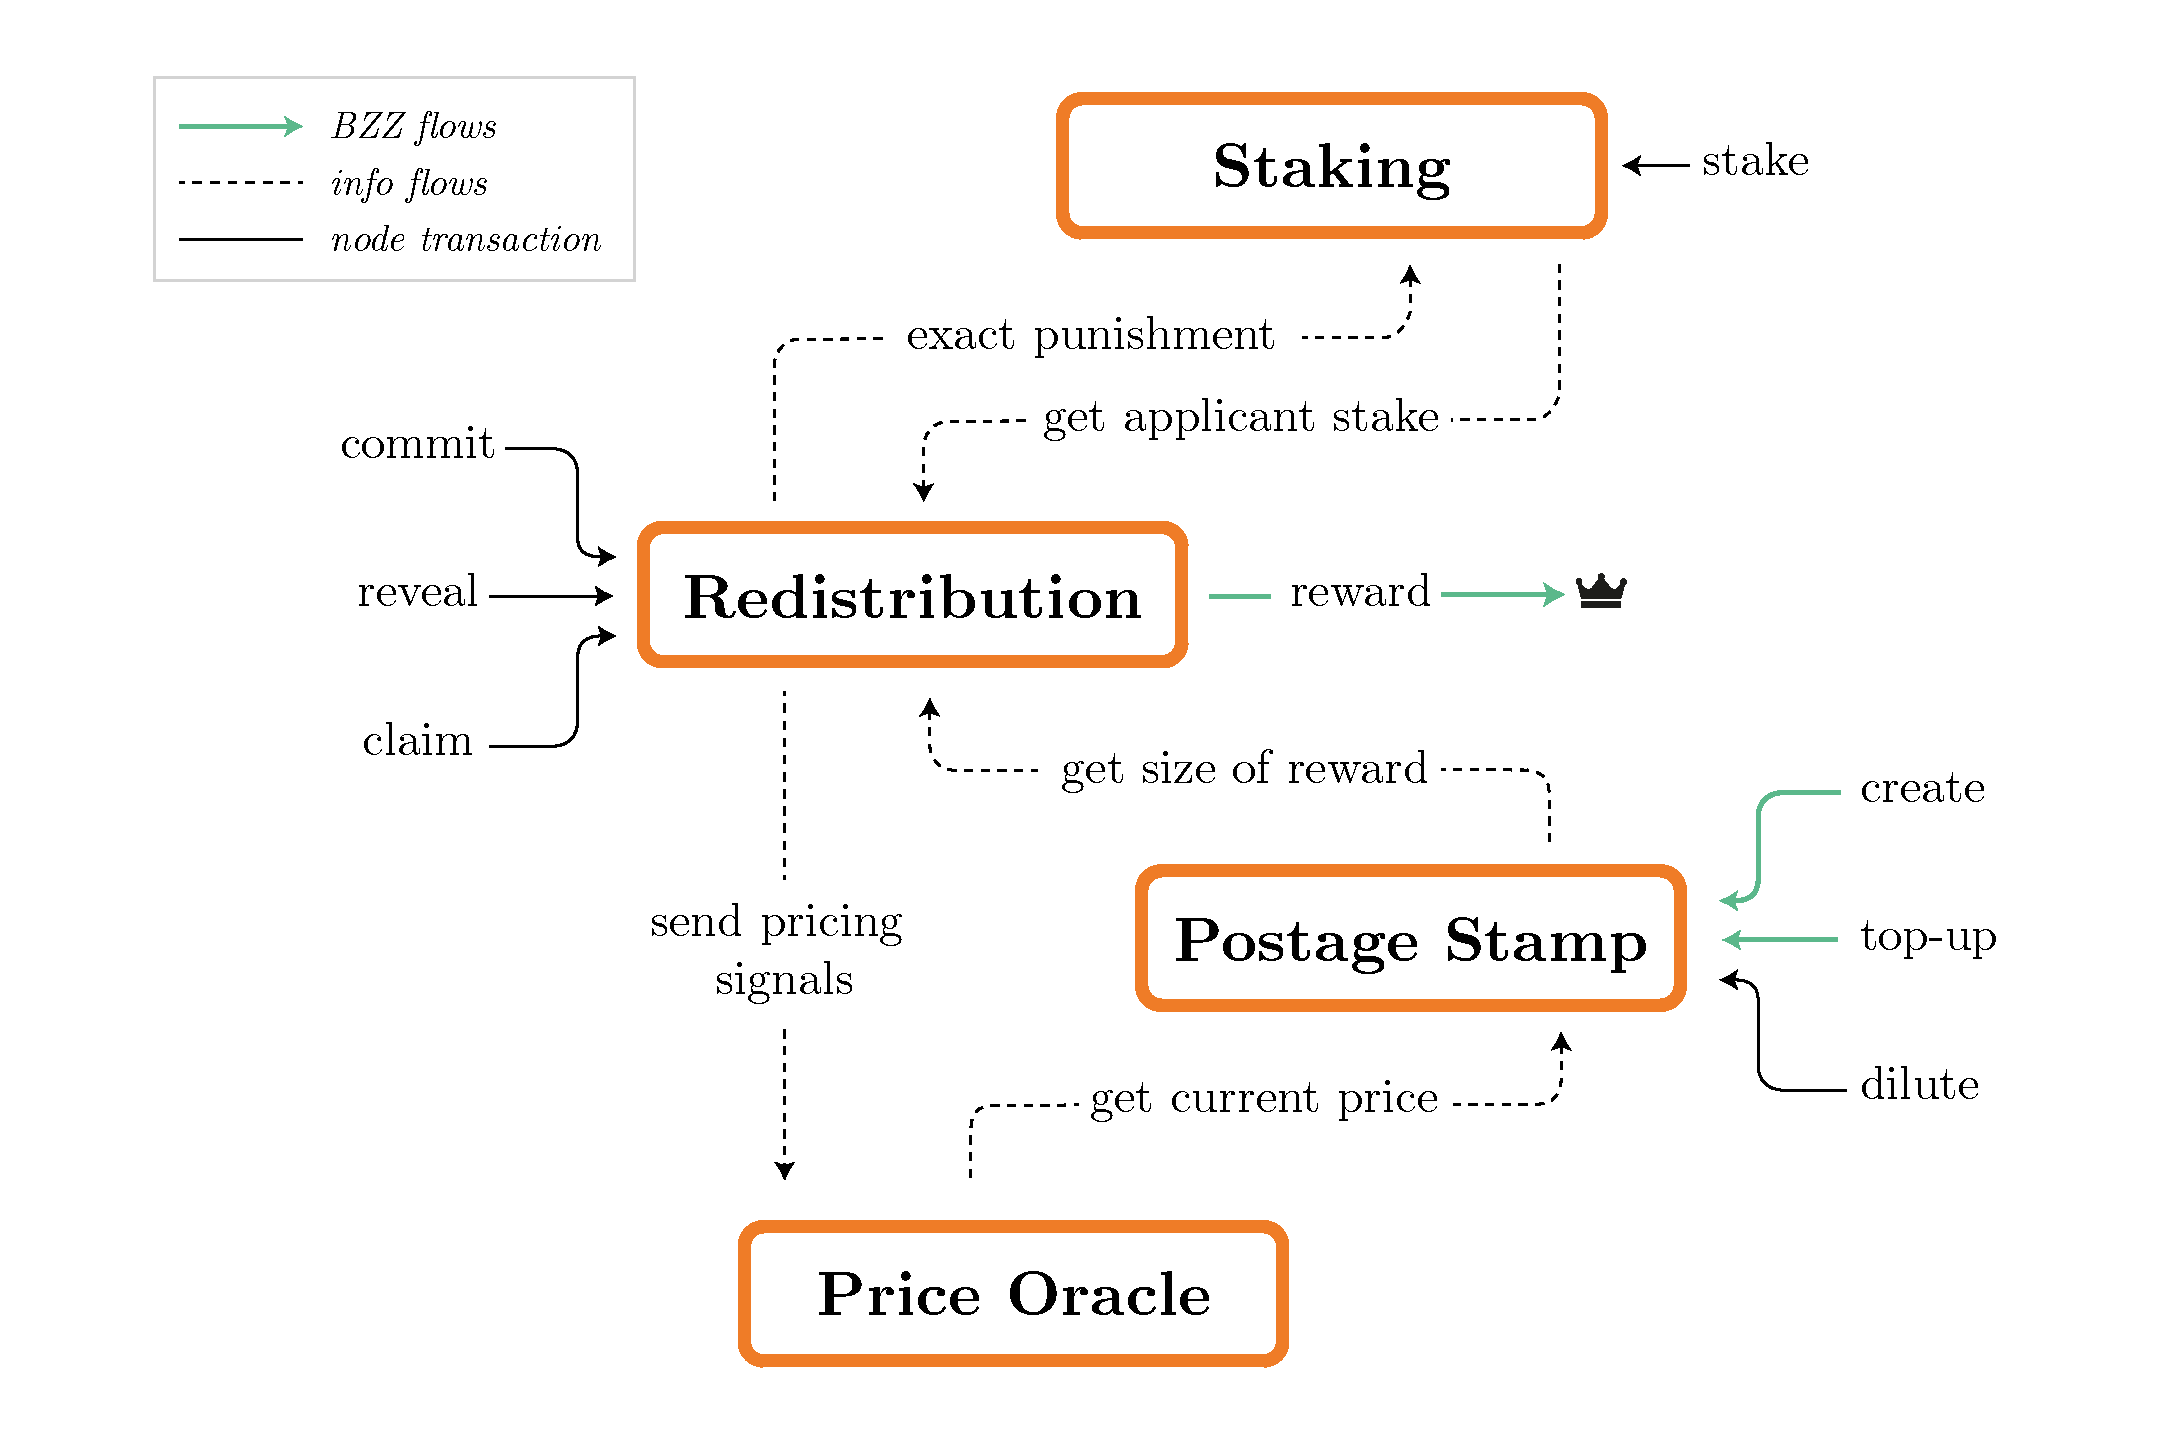
\includegraphics[width=\textwidth]{fig/smart contract interaction.pdf}
  \caption[Interaction of smart contracts for swarm storage incentives]{Interaction of smart contracts for swarm storage incentives. The figure shows with the dotted line the information flow between the four contracts comprising the storage incentive smart contract suite as well as the public transaction types they accept. }
\label{fig:smart-contracts}
\end{figure}    

The game is structured as a sequence of \emph{rounds}. Each round lasts for a fixed number of blocks and recur periodically. A round consists of 3 phases: \emph{commit}, \emph{reveal}, and \emph{claim}.%
%
\footnote{The commit and reveal phases are one quarter of the round length while the claim phase is one half.
}
%
The phases are named after the type of transaction the smart contract expects during that phase, and that nodes from the selected neighbourhood need to submit.%
%
\footnote{Both commit and reveal are simple and cheap transactions. The only expensive transaction is claim but that only the winner needs to submit.}
%
See figure \ref{fig:phases}

\begin{figure}[!ht]
  \centering
    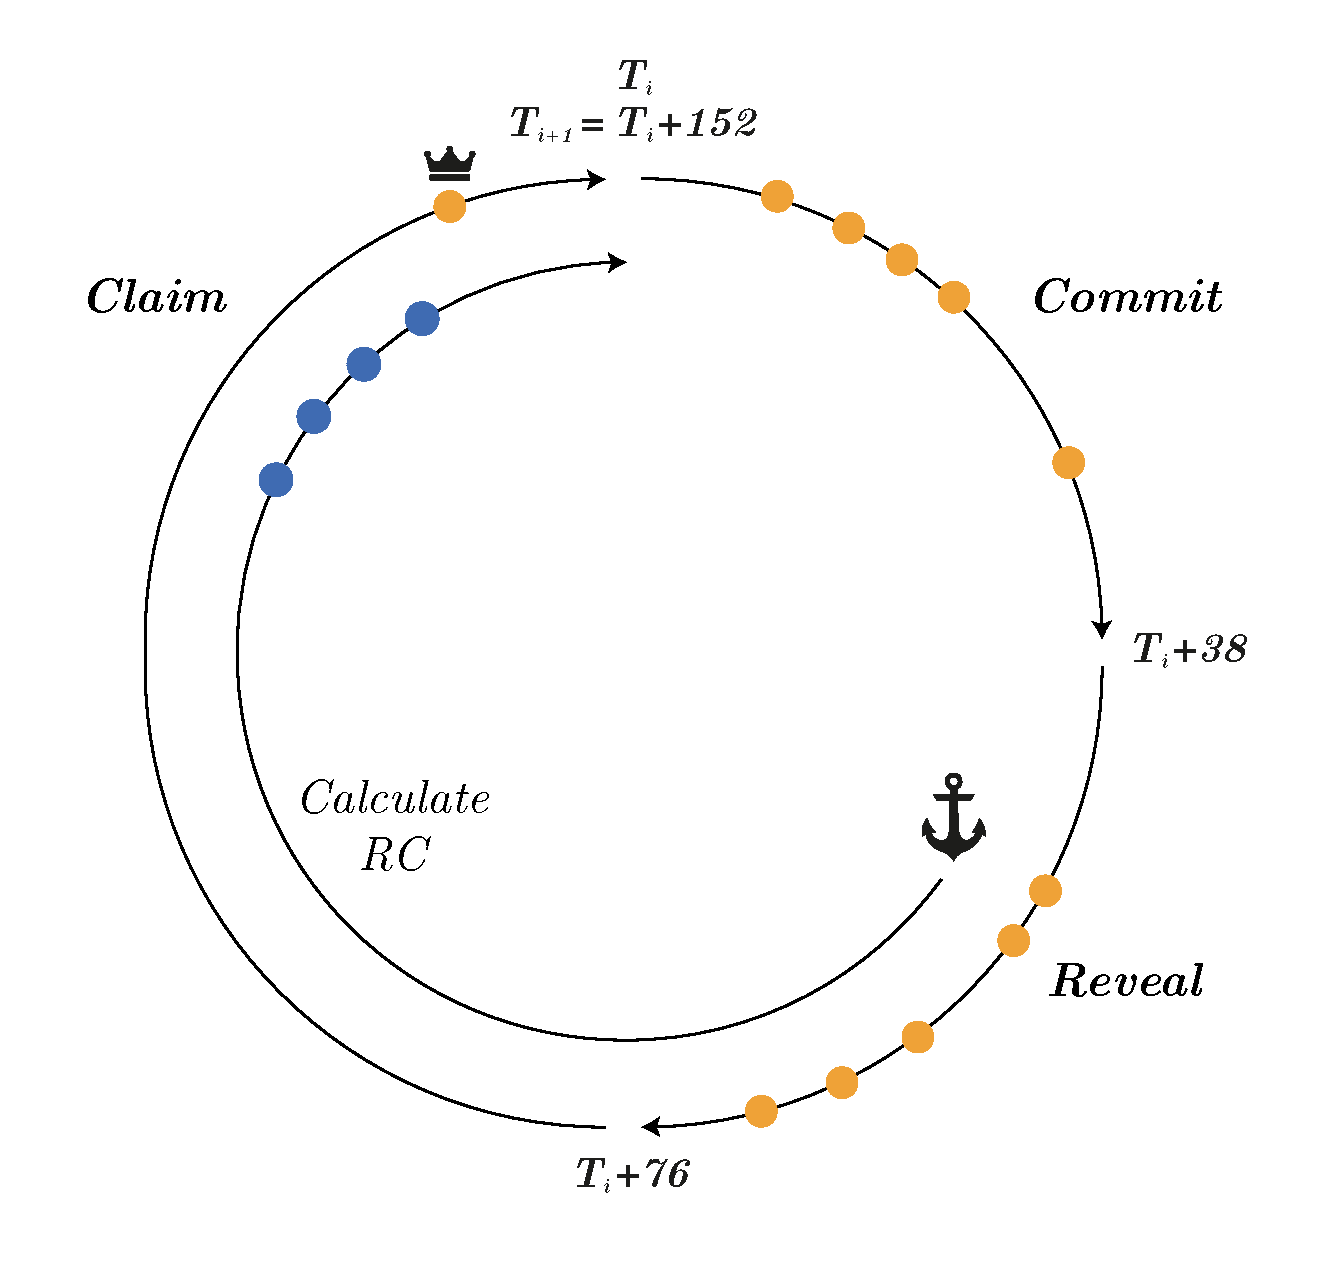
\includegraphics[width=.5\textwidth]{fig/round lifecycle copy.pdf}
  \caption[Phases of a round of the redistribution game]{Phases of a round of the redistribution game. The figure displays the timeline of the repeating rounds of the redistribution game with its phases. In the context of smart contract interaction, logically starting with the commit phase, followed by reveal and claim. From the point of view of client node engagement starting with the end of the reveal phase with the neighbourhood selection anchor revealed, those in the selected neighbourhood start calculating their reserve sample only to submit it by the end of the next commit phase. If they are selected as an honest node and as a winner, they submit their proof of entitlement in a claim transaction.}
\label{fig:phases}
\end{figure}    

Once the reveal phase is over, the  \emph{neighbourhood selection anchor} becomes known. Nodes that have the anchor within their neighbourhood%
%
\footnote{If storage depth is less than the anchor's proximity order relative to the overlay address.}
%
are  allowed to participate in the following round (see figure \ref{fig:neighbourhood-selection}).



The storer nodes in a neighbourhood are assumed to have  consensus over the chunks that make up their reserve and provide evidence called \emph{proof of entitlement} to the blockchain (discussed below in detail in \ref{sec:por}). In such a game, the Nash-optimal strategy for each node is to follow the protocols and coordinate to guarantee that from the same information, all neighbouring peers will arrive at the same proof of entitlement. Since the proof of entitlement needs to be consensual but unstealable,%
%
\footnote{%
Any explicit communication between independent nodes about this reserve before the end of the commit phase constitutes risk in that it may leak the proof to a node not doing storage work. Therefore nodes are incentivised to keep the proof a secret. Making these proofs unstealable helps detect opportunistic peers that pose as storers but do not provide adequate storage.}
%
a commit/reveal scheme must be used.

In the commit phase, nodes in a neighbourhood will apply by submitting the \emph{reserve commitment} obfuscated with an arbitrary key that they later reveal (see definition \ref{def:chc} in appendix \ref{sec:appendix-game}). The smart contract receiving the commit transaction verifies that the node is staked, i.e., the registry of the staking contract contains an entry for the node's overlay with a stake that is higher than the minimum stake.

In the reveal phase, each node that previously committed to a reserve, now reveal their commitment by submitting a transaction containing
their reserve commitments, their storage depth,
their overlay address, and the key they used to obfuscate  the commit.
When receiving the reveal transaction, the contract  verifies that the revealed data serialised does indeed hash to their commitment. It is also checked if the node belongs to the neighbourhood designated by the neighbourhood selection anchor, i.e., is within the storage depth provided in the reveal.

In the claim phase, the winner node must submit a claim transaction.%
%
\footnote{Every node in the selected neighbourhood needs to perform the corresponding calculations to determine whether or not they are the winner.}
%
First, in order to decide the outcome of the Schelling game, one reveal is selected  from among the reveals submitted during the reveal phase.%
%
\footnote{This is relevant only if the depth and/or the commitment are non-uniform across applicants.}
%
The selected reveal represents the truth; the set of applications agreeing with the selected one represent the \emph{honest peers} of the neighbourhood, the ones disagreeing are the \emph{liars}, while those committers that did not reveal or revealed invalid data are the \emph{saboteurs}. Honesty is incentivised by the fact that liars and saboteurs get punished. In what follows we introduce staking that is needed for both the selection processes and the punitive measure.


\subsection{Staking}\label{sec:staking}

\subsubsection{Neighbours with shared storage}

In order to provide robust protection against accidental node churn, i.e., ensure retrievability of chunks from a neighbourhood in the face of some nodes being offline, the swarm require a number of independent storers in each neighbourhood physically replicating content.
If payout was given to each node that shows proof of entitlement, then operators would be incentivised to create spurious nodes with the sole purpose of applying for the reward. Measures can be introduced to enforce that these spurious nodes must be operating on the network, but ultimately, operators may choose to actually run several nodes yet share their storage on a single hardware. 
The incentive system must ensure that storage providers do not  adopt this strategy. To this end, we introduce \emph{staking}.  

Stakes are used as weights by the contract to determine the true reserve commitment (truth selection) as well as the winner among the honest nodes (winner selection). Since peers' relative stake determine their chance of winning, stake is additive, i.e., operators' profit only depends on their total stake within the neighbourhood. Given the cost of running a node, operators will have no  motivation to divide their stake between multiple nodes sharing storage hardware.



\subsubsection{CommiTted stake and stake balance}

When registering in the staking contract, stakers commit to a stake denominated in rent units called 
\emph{committed stake}.  The committed stake must have a lower bound.%
%
\footnote{A large number of staked nodes could cause the claim transaction to fail due to gas cost needed for iterating over them. This presents a potential attack where the adversary registers stakes for many nodes and commits for all of them. Such an attack is made prohibitively costly by enforcing a minimum stake.}
%
The  amount sent with the transaction is recorded and serves as collateral called \emph{stake balance}. Stakes can be created or topped up any time, but the update time is recorded together with the amount.
Participation is restricted to peers whose stake has not changed recently, thereby excluding the possibility of changing stakes after knowing the selected neighbourhood.
Every time the stake of a node is queried, the contract returns  the  absolute committed stake in BZZ calculated as (1) the committed stake in rent units multiplied by the unit price of rent  or (2) the entire stake balance, whichever is smaller (see definition \ref{def:stakes} in appendix \ref{sec:appendix-game}).  

Stakes must be transferrable between overlay addresses to facilitate neighbourhood hopping in case the distribution of stake per neighbourhood is unbalanced. 

\subsubsection{Withdrawability of surplus stake balance}



The committed stake lets operators express their  profit margin together with time preference for realising this profit. Since the profit is only transparent once the relative stakes within the neighbourhood are known, it is possible that nodes take a while to discover their optimal stake. 

If the BZZ token price increases and the unit price of rent drops, the entry for the node in the stake registry will show excess balance. This surplus can always be withdrawn,
and, as a consequence, stakers can realise their profit from BZZ appreciation.%
%
\footnote{In case the token price goes up substantially, the stake balance ends up worth much more than what nodes can ever expect to earn. If the stake balance was not at all withdrawable, participation would be disincentivised due to fear of losing the potential gains in the event of BZZ token appreciation.}
% 

 
%%%%%%%%%%%%%%%%%%%%%%%%%%%%%%%%%%%
\subsection{Neighbourhood consensus over the reserve}\label{sec:por}

Peers applying for the round must agree on which chunks belong to their respective reserves. For this, at the very least, the applicants must consent on their area of responsibility, which can be derived from their storage depth and their overlay address.  
The consensus over the reserve content is tested with the identity of a \emph{reserve sample}.
The sample is the first $k$ chunks in the reserve using an ordering based on a modified hash of the chunks (see \ref{def:transformed-reserve} in appendix \ref{sec:appendix-game}).  The modified chunk hash is  obtained using the chunk contents and a \emph{salt} specific to the round.%
%
\footnote{This modified hash is the BMT hash of the chunk data using Keccak-256 prefixed with the reserve sample salt as a base hash (defined in \ref{def:prefixed-hash} in appendix \ref{sec:appendix-game}). The ordering is the ascending integer order reading the 32-byte modified hash as a big endian encoded 256-bit integer (see \ref{def:sampler} in appendix \ref{sec:appendix-game}).}
%
It is impossible for any node to construct this set unless they store all (or a substantial number of the) valid chunks together with their data at or after the time the salt is revealed. 

\subsubsection{Recency and sampling}

The reserve sample must exclude too recent chunks because, otherwise, malicious uploaders could bombard nodes in the neighbourhood with a non-identical set of chunks  that are going to be sampled thereby breaking the consensus about the reserve. One way to guard against this attack is to save each chunk together with its time of storage%
%
\footnote{Using the timestamp within the postage stamp to define the minimum age on would not solve the consensus problem since chunks with old postage stamp could be circulated towards the end of sampling and cause disagreement between neighbours.}
% 
in the local database.
Pairwise synchronisation of chunks between neighbours with the pull-sync protocol respects this ordering by time of storage. 
We require that live syncing, i.e., syncing of chunks received after the peer connection started has a latency not longer than an agreed constant duration called \emph{maximum syncing latency} (or \emph{max sync lag} for short). Peer connections lagging more with syncing are by protocol not counted as legit storer nodes. This restriction ensures that malicious nodes can not back-date new chunks more than the max sync lag without losing their storer status. 

In order to reach consensus, we must ensure that all chunks received by any node in the neighbourhood not later than $l$ should reach every node of the neighbourhood before the claim phase.
% This means that after receiving the chunk with a lag, the client still has time to include it in their sample and safely submit the commit transaction.
%
If we choose $l$ as 2 times the allowed sync lag then every chunk landing first with a node has time to arrive at each node to be safely included in a consensual sample.%
%
\footnote{Instead of actually monitoring neighbour connections and abstain from committing to a sample in case of excessive lag, one can just choose a small enough sample size.}%
%

\subsubsection{Storage depth and honest neighbourhood size}

In order to decide which reveal represents the truth for the current round, one submission out of all reveals is selected randomly with a probability proportional to the amount of stake the revealer has. More precisely: the amount of stake per neighbourhood size, i.e.,    \emph{stake density}. The reserve sample hash and the reported storage depth thus revealed are considered the truth for the current round. 

Now we can understand why nodes will report actual storage depth correctly. If a node chooses to play with a larger neighbourhood than the neighbours, it will be selected more often than the others. However, as the committed storage depth decreases as compared to peers, the node's stake is counted with an exponentially deflated  value relative to the peers reporting a deeper storage radius, making such an attack costly.  

Overreporting storage depth is possible as long as the the node falls into this narrower proximity of the neighbourhood selection anchor. Therefore, a systematic exploit requires the malicious actor to control a staked node in each subneighbourhood of the true honest neighbourhood. 
On top of this, the winners also need to show evidence that the set of chunks within their storage depth do fill their reserve. 
The actual integer values of the transformed chunk addresses in the sample hold information regarding the size of the original sampled set.  
Requiring the size of the sampled set to fall within the expected range (with sufficient certainty) translates to imposing a constraint on the upper bound of the values of the sample. This construct is called \emph{proof of density} (see definition \ref{def:chunk-density-validition} and appendix \ref{sec:density}).
%

Note that the sample-based density proof can be spoofed if the attacker is mining content filtering chunks in such a way that the transformed chunk addresses form a dense enough sample, then uses its own postage batches to stamp them. 
Further hardening against such attacks can be achieved by requiring  additionally a commitment to the entire set of postage stamps and similarly proving from a randomised sample the custody of a sufficient quantity. Due to this requirement, fraudulent claimants must not only generate the content, but must also have enough storage slots to fake the sample. This would require the attacker to purchase postage batches in the magnitude of the entire network 
or keep track of and store the actual postage stamps existing in the network. The former imposes a prohibitive cost on the attacker, whereas, in the latter case, the malicious claimant must bear the risk of relying on honest  neighbours for the post-hoc retrieval of witness chunk data needed for the proof of entitlement.
% See figure \ref{fig:proof-of-density}

% \begin{figure}[!ht]
%   \centering
%     % \includegraphics[width=\textwidth]{fig/rproof-of-density.pdf}
%   \caption[Proof of density]{Proof of density.}
% \label{fig:proof-of-density}
% \end{figure}    


\subsubsection{Skipped rounds and rollover}

If there is no claim in a given round, the pot simply rolls over and increase the outpayment for the next round of the redistribution. This policy is by far the easiest to implement, resulting in the lowest gas expenditures.% 
%
\footnote{One might argue for reimbursing honest nodes for their transaction costs. Thereby,  nodes with really small stakes can still participate and in general nodes are less exposed to variance in the probabilistic outpayments.}

\subsubsection{The eight rules of entitlement}

Here we summarise the eight rules of validating a claim (with committing and revealing a reserve commitment and then submitted evidence as proof of entitlement; see also table~\ref{tab:gr8}):%
%
\footnote{The first three criteria are part of the conditions for staking, committing, and revealing (see definitions \ref{def:chc} and \ref{def:chs} for replication, \ref{def:stakes} and \ref{def:commits} for redundancy, \ref{def:reveals} for responsibility in appendix \ref{sec:appendix-game}. Relevance, retention, recency and  retrievability are proved as part of the proof of reserve (definition \ref{def:por}) and validated as part of the claim (\ref{def:por-validation}). Finally, proof of resources involves density proofs for chunks and stamps (definitions \ref{def:chc} and \ref{def:chs}) validated as part of the claim (definitions \ref{def:chunk-density-validition} and \ref{def:stamp-density-validition}, respectively). The specific construct of proof of entitlement is defined in \ref{def:poe} and its validation in \ref{def:claim-validation} in appendix \ref{sec:appendix-game}).}
%
\begin{itemize}[noitemsep]
%
\item[\hbox to 2em{\textsc{replication}}] \hspace{1cm}\\ Since liars get frozen (i.e., nodes that had revealed reserve commitment hash or storage depth different  from the winner are excluded from the game for a period), nodes in a neighbourhood are incentivised to replicate their reserve by syncronising the chunks they store using the pull-sync protocol.
%
\item[\hbox to 2em{\textsc{redundancy}}] \hspace{1cm}\\ The stake is used as weights in determining the within-neighbourhood probability of a node being selected as winner (see \ref{def:winner-selection}). This implies no benefit in submitting multiple claims. Operators running multiple nodes in one neighbourhood (sharing storage) therefore have no advantage over running a single node with the same total stake. Assuming this disincentive to proliferate is effective, staking can be regarded as guarantee for true redundancy.
%
\item[\hbox to 2em{\textsc{responsibility}}] \hspace{1cm}\\  At the time of revealing it is checked if the neighbourhood selection anchor falls within the node's radius of responsibility, i.e., belong to the covered range of addresses whose proximity to the node's overlay address is not less than their reported storage depth. 
%
\item[\hbox to 2em{\textsc{relevance}}] \hspace{1cm}\\ Using a witness proof with the reserve commitment hash as root, we show evidence that an arbitrarily chosen segment in the reserve sample packed address chunk is the address of a witness chunk. 
A valid postage stamp signed off on this witness chunk address is presented to show that storing that chunk  in the reserve is relevant to someone (and is paid for). 
\item[\hbox to 2em{\textsc{retention}}] \hspace{1cm}\\ A segment inclusion proof is provided as evidence that the chunk data has been retained in full integrity. 
\item[\hbox to 2em{\textsc{recency}}] \hspace{1cm}\\ The salt used for the transformed reserve sample is derived from the current round's random nonce proving that the RS must have been compiled recently. The witness and segment indexes are derived from the next game's random seed ensuring that at the time of compilation and commitment, no compressed or partial retention of chunk data would have been
sufficient.
\item[\hbox to 2em{\textsc{retrievability}}] \hspace{1cm}\\  The chunk is shown to be retrievable by proximity based routing, i.e. its address belongs to the range of addresses covered by the neighbourhood: the chunk's proximity order to the node's overlay address is not less than their reported storage depth. 
\item[\hbox to 2em{\textsc{resources}}] \hspace{1cm}\\ Resource retention checks the volume of resources constituting the reserve by estimating the sampled set size via chunks density and stamps density. 
\end{itemize}


{\small \begin{longtable}{l|p{.4\textwidth}|p{.4\textwidth}}
\toprule
 {proof of} & {construct used} & {attacks mitigated}\\\midrule
 \textsc{replication}& Shelling-game over reserve sample& non-syncing, laggy syncing\\
 \textsc{redundancy}& share of reward proportional to stake & shared storage, over-application\\
 \textsc{responsibility}& proximity to anchor & depth/neighbourhood misreporting \\
 \textsc{relevance}& scarcity of postage stamps & generated data \\
 \textsc{retention}& segment inclusion proof & non-storage, partial storage\\
 \textsc{recency}& round-specific salt for reserve sample & create proof once and forget data\\
 \textsc{retrievability}& proximity of chunk & depth over-reporting\\ 
 \textsc{resources}& density-based reserve size estimation & targeted chunk generation (mining) \\\bottomrule
  \caption[r8: proofs used as evidence for entitlement to reward]{r8: proofs used as evidence for entitlement to reward.}
\label{tab:gr8}
 \end{longtable}
 }


\subsection{Pricing and network dynamics}\label{sec:price-oracle}

In this section, we first put the redistribution scheme in the context of self-sustainability, and provide a simple solution for price discovery.

For Swarm to be a truly self-sustaining system, the unit price of storage rent must be set in a way that is responsive to demand and supply. Ideally, the price is automatically adjusted based on reliable signals resulting in dynamic self-regulation. The guiding insight here is that the information storer nodes provide when  they apply for the redistribution game, also serves as a price signal. In other words, the redistribution game serves as a decentralised price oracle.



\subsubsection{Splitting and merging of neighbourhoods}

The storage depth represents the proximity radius within which the neighbourhood's storer nodes keep all chunks with valid postage stamps and fill their reserve. 


If the volume of newly issued storage slots from recently purchased batches (\emph{ingress rate}\/) and the volume of expired storage slots (\emph{outgress rate}\/) balance out, the storage depth remains unchanged.
But see what happens  if the volume of  reserved chunks increase?
Now, since the client's reserve capacity is constant, after a while, nodes are able to fill up their capacity with chunks that are at most one proximity order closer to them than the farthest chunks were previously, i.e.,  their storage depth increases.
When the volume of reserved chunks doubles,  the storage depth increases by one.  

In order to store this excess data under the same redundancy constraints the network requires double the number of nodes. If all else is equal, double the network-wide reserve, double the postage revenue and therefore double the overall pot that gets redistributed. When neighbourhoods split as they are absorbing the new volume, they simultaneously release the chunks in the PO bin of their old depth, i.e., the chunks now stored by their sister nodes. 

Utilisation rate is an organic way to  introduce pressure against fully maxing out a node's reserve with critical content, and thereby enable early detection of capacity pressure. This provides  sufficient safety buffer for the triggered incentives to take effect. For instance,  if utilisation rate is $1/8$, the storage depth is up to 3 PO-s shallower than the reserve depth.%
%
\footnote{The narrative of this scenario is that uploaders with underutilised batches subsidise extra redundancy for everyone.}
%
Now the ingress can be really high and bring the reserve depth down to storage depth. When the tendency of a closing gap between the potential (reserved) and actual (observed) utilisation of the DISC is detected, any incentive change will have the buffer to take effect without target redundancy being threatened. 

% See figure \ref{fig:pricing-demand}.


% \begin{figure}[!th]
%   \centering
%     % \includegraphics[width=.5\textwidth]{fig/pricing-demand.pdf}
%   \caption[Batch utilisation rate as a price signal]{Batch utilisation rate as a price signal.}
% \label{fig:pricing-demand}
% \end{figure}


\subsubsection{Number of honest nodes as price signal}

Since the storage capacity is maxed out, the ratio of supply and demand is directly seen in the number of honest nodes playing the Schelling game. 

We assume that if nodes are staying in the network for a longer period, their doing so testifies to their profitability. For a stable swarm, neighbourhoods need only 4 (balanced) nodes within as neighbourhood. Assuming equal stake (or more precisely, assuming that relative stake equalises profitability of node operators) if there are $n$ nodes in a neighbourhood, their long term profit is equally shared, this amount is optimised if there are exactly four nodes ($n=4$). This number can be more, since opportunistic operators may start their nodes in a complete neighbourhood in anticipation of a neighbourhood split due to capacity demand. As these nodes stay in, the same long term winnings of the neighbourhood gets distributed among more nodes than optimal.
However, the fact that nodes tolerate this implies that the reward is too much (the price is too high), and the network can tolerate a decreasing price.

On the other hand, if the number of honest revealers is less than the neighbourhood redundancy requirement, it signals capacity shortage and therefore requires the storage rent to increase. 

% See figure \ref{fig:pricing-supply}.

% \begin{figure}[!th]
%   \centering
%     % \includegraphics[width=.5\textwidth]{fig/pricing-supply.pdf}
%   \caption[Price signal for supply of storage capacity] {Price signal for supply of storage capacity.}
% \label{fig:pricing-supply}
% \end{figure}


\subsubsection{Parameterisation of the price oracle}

The rule for updating the price from one round to the next is that the current price is multiplied by a value $m$ which depends on the number of honest revealers in the round (formally defined in appendix \ref{sec:appendix-price-oracle}). Mathematically, $p_{t+1} = m p_t$, where $p_t$ is the price in round $t$ (and $p_{t+1}$ is then the price in the following round). We define the multiplier $m$ in terms of the number of honest revealers $r$ and a stability parameter $\sigma$ governing how quickly the price should increase or decrease, all other things equal. 

\begin{figure}[!ht]
  \centering
  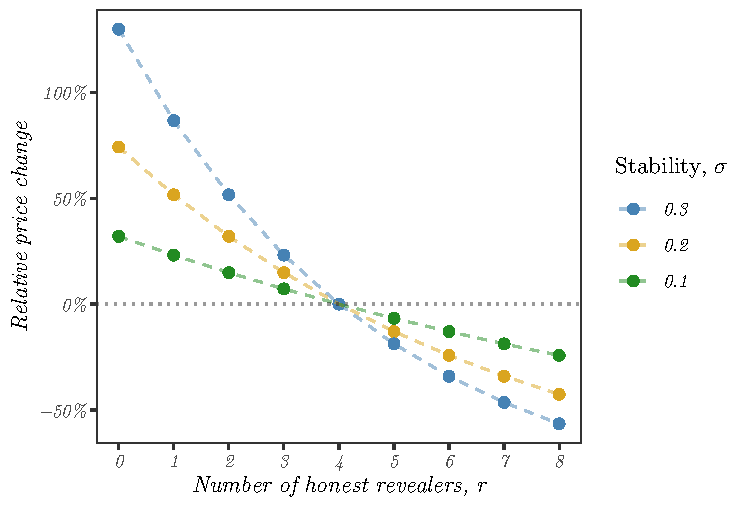
\includegraphics[width=.7\textwidth]{fig/adaptive-pricing.pdf}
  \caption[Adaptive pricing] {Adaptive pricing. The relative change in price (y-axis), mathematically expressed as the price in the next round divided by the price this round minus one ($p_{t+1} / p_t - 1$), is displayed against the number of honest revealers $r$ in the current round (x-axis). This is done so for three different values of the stability parameter $\sigma$ (colours). The points are the actual price change values; the connecting dashed lines are for visual aid only. The dotted horizontal line highlights the point at which no price change happens. Price change is exactly zero for any $\sigma$ when the number of honest revealers is four. Otherwise, larger values of $\sigma$ lead to larger relative price changes as the number of honest revealers is varied.}
  \label{fig:adaptive-pricing}
\end{figure}

In particular, we choose $m = 2^{\sigma(4 - r)}$, and therefore we have $p_{t+1} = 2^{\sigma(4 - r)} p_t$. This expresses how the deviation $4 - r$ of the number of revealers from the optimal value of 4 maps to an exponential change in price. The stability parameter $\sigma$ determines the generic smoothness of price changes across rounds, i.e., how many rounds it takes for the price of rent to double in case of a consistent signal of the lowest degree of undersupply (or halve in case of a consistent oversupply). Figure \ref{fig:adaptive-pricing} illustrates how the price model works.

Two minor adjustments are applied to this simple model. First, $r$ is capped at some value $r_{\text{max}}$ (chosen to be 8 in our case). That is, $r$ should actually be interpreted as the minimum of the number of honest revealers and $r_{\text{max}}$. Second, the price is never allowed to drop below some predetermined minimum $p_{\text{min}}$. That is, in case the price drop from one round to the next would bring the price below $p_{\text{min}}$, it will instead be kept at $p_{\text{min}}$. 



\section{Conclusion}


% \subsection{Evaluation}

In this paper we presented and formalised a system of positive incentives for chunk storage in Swarm. This section summarises its features and analyse its benefits.%
%
\footnote{The areas left for future directions of research include: truely anonymous and leakless uploads with mixing postage stamps; guarantee period of availability and fixed price with \emph{bzz future providers}; \emph{non-compensatory content insurance} as a network service; parallel games; and last but not least finding an alternative to non-withdrawable stake for ensuring rendundancy.}

\subsubsection{Fair}                                           
The incentive system provides a fair distribution scheme, i.e., on average storer nodes receive compensation in proportion of their contribution to overall storage work performed by the swarm network in total. The amounts paid out depend on the time since the last payout and the total storage volume in the network.
The rent deduced from batch balances is proportional to the time since the last payout and to  storage volume purchased, 
thus making storage rent fair on uploaders. 
                
% The variance in the interval between outpayments is limited and not sensitive to the highly variable new batch ingress rate.
% Also thanks to collective payout to neighbourhoods, the variance of individual nodes is decreased, an effect similar to mining pools in proof of work blockchains.



\subsubsection{Adaptive}

The incentive system is adaptive to changing network size, data ingress rate and overall storage volume. 

It achieves economic sustainability through self-regulating profitability by dynamically adapting the unit price of storage rent following signals of supply and demand. 

\subsubsection{Inexpensive}

The system does not require any operator input, does not induce extra computational work, and incurs only minimal overhead in network traffic and storage. No significant upfront capital or advance registration is required to keep the barrier of entry low. 

The reward is paid out upon submission of a valid claim directly verifiable by the smart contracts on the blockchain. The blockchain component does not require historical bookkeeping or managing registrations, and does not rely on challenges, or time-sensitive (frontrunnable) competition. Transaction cost is kept low so that the cost of required on-chain transaction do not impact the profitability of a storer node.

\subsubsection{Robust}

The system is conceptualised using requirements and corresponding evidence, which allows easier reasoning about resilience against exploits such as collusion, grieving/trolling, node and chunk proliferation attacks. 

The system is resilient to swarm usage patterns - not sensitive to variance or other properties of ingress volumes per period, file sizes or postage batch size, number of  batches, their balances and their owners.

% \subsection{Remaining problems and future work}
% \subsubsection{Anonymous and leakless uploads}
% Mixing postage stamps 
% \subsubsection{Guaranteed expiration}
% future providers
% \subsubsection{Content insurance}
% compensatory or staked insurance - receipts and litigation
% \subsubsection{Doing without stake}

% Such sybil nodes with shared storage are prevented by requiring participants to operate multiple \emph{sister nodes}, each in a different neighbourhood. The same public key would derive a number of overlay addresses. The storage redistribution requires a single proof of participation with proof of reserve size from each sister neighbourhood to be attached to the winning claim. This enforces storage providers to run all sister nodes.


% Operating sybil nodes with shared storage is less profitable the more sister nodes we require unless the sister node is also a sybil node without storage. While this can be arranged by mining addresses, we can also make it ineffective if we distribute the reward equally based on distinct sisters.


% \bibliography{refs.bib}

\newpage


% \phantomsection 
\appendix
\addcontentsline{toc}{section}{Appendix}
\section*{Appendix}
\renewcommand{\listtheoremname}{List of definitions and theorems}
\enlargethispage*{\baselineskip}
% {\small
\listoftheorems[ignoreall,show={definition,corollary,lemma,theorem}]
% }
\section{Formal specification}\label{sec:formal}

\subsection{DISC basics}\label{sec:appendix-disc}
\subsubsection{Notation}

\begin{itemize}[noitemsep]
    \item  $\mathrm{roman}$ -- predicates standing for blockchain verifiable properties 
    \item \textsc{smallcaps}-- field of a composite, tuple member function
    \item $\Pi^p$ -- proof constructor function
    \item $\mathbb{V}^p$ -- validator function
    \item \texttt{TT\_FONT} -- constant parameter (see appendix \ref{sec:constants})
    \item $\mathit{uint}[d]$ -- left closed, right open integer range $\overline{\left[0,2^d\right)}$
\end{itemize}


\subsubsection{Sequences}
 
\begin{definition}[sequences \statusgreen]
Define $\tau\{n\}$, the non-polymorphic sequences of length $n$ (non-negative) over any type $\tau$ as an indexing function:
%
\begin{eqnarray}
\tau\{n\} &\defeq& \begin{cases}\nil&\text{ if } n=0\\
\overline{0,n-1}\mapsto \tau &\text{ if } n>0
\end{cases}\\
\tau{+}&\defeq&\bigcup_{n\in \mathbb{Z}^{+}} \tau\{n\}\\
\tau{*}&\defeq&\{\nil\}\cup\tau{+}\\
\end{eqnarray}
%
Length function $\mathit{len}$:
\begin{eqnarray}
\mathit{len}(s)&:&\tau\mapsto\mathit{uint64} \\
\mathit{len}(s)&\defeq& \begin{cases}
0 & \text{ if  } s=\nil\\
n & \text{ if  } s\in\tau\{n\}
\end{cases}
\end{eqnarray}
%
The positional index 'at' function:
\begin{eqnarray}
\idx{}&:&\tau*\mapsto\times\mathit{uint64}\mapsto\tau\\
s\idx{}&:&\overline{0,\mathit{len}(s)-1}\mapsto\tau\\
s\idx{i}&\defeq&s'(i)   
\end{eqnarray}
%
Define the \emph{concatenation} operator '$\concat$':
\begin{eqnarray}
(x\concat y)&:& \overline{0, \mathit{len}(x) + \mathit{len}(y)-1}\mapsto\tau\\
(x\concat y)\idx{i} &\defeq& \begin{cases}x\idx{i} & \text{ if  } 0\leq i< \mathit{len}(x)\\
y\idx{i-\mathit{len}(x)}&\text{ otherwise } 
\end{cases}
\end{eqnarray}
%
Define slices (subsequences) with the range operator '$\rangedel$':
\begin{eqnarray}
(s\idx{o\rangedel o+l})&:&\overline{0, l-1}\mapsto\tau\\
(s\idx{o\rangedel o+l})\idx{i}&\defeq&s\idx{o+i} 
\end{eqnarray}
where 
\begin{eqnarray}
o, l \geq 0\land\\
\mathit{len}(x)\geq o+l
\end{eqnarray}
%
Let us also define empty, prefix and suffix slices:
\begin{eqnarray}
s\idx{x\rangedel x} &\defeq& \nil\\
s\idx{\rangedel x} &\defeq& s\idx{0\rangedel x}\\        
s\idx{x\rangedel}  &\defeq& s\idx{x\rangedel \mathit{len}(s)}
\end{eqnarray}
\end{definition}
%
As a special case byte slices are defined as sequences of 8-bit integers.
%
\begin{definition}[segmentation]
\label{def:segmentation}
Define segment as an at most 32 long byte slice, and define  segmentation of a slice of bytes as the partitioning of the slice into consecutive segments. 
%
Define segment count as the number of segments that cover a byte slice:
\begin{eqnarray}
\mathit{SegCnt}&:&\mathit{byte}*\mapsto\mathit{uint64}\\
\mathit{SegCnt}(s)&\defeq&\mathit{int}\left(\frac{\mathit{len}(s)-1}{32}\right)+1 
\end{eqnarray}
%
Now we can define the segment indexing function 
$\idx{\idx{}}$ which maps the byte slice $s$ and an index $i$ to the $i$-the segment in the segmentation of $s$:
\begin{eqnarray}
\idx{\idx{}}& : & \mathit{byte}{*}\mapsto\mathit{uint64}\mapsto\mathit{Segment}\\
s\idx{\idx{}}&:&\overline{0,\mathit{SegCnt}(s)-1}\mapsto\mathit{Segment}\\ 
s\idx{\idx{i}}&\defeq&\begin{cases}s\idx{32\cdot i\rangedel} &\text{ if } i = \mathit{SegCnt}-1\\
s\idx{32\cdot i\rangedel 32\cdot(i+1)} &\text{otherwise}
\end{cases}
\end{eqnarray}
\end{definition}

\subsubsection{Custom types}


\begin{definition}[Swarm overlay address of node $n$]\label{def:overlay}
%
A Swarm node is associated a Ethereum account that the node operator must possess the private key for, called \emph{bzz account} ($K_n^\mathit{bzz}$). The node's overlay address is derived as the hash of the binary serialisation of the Ethereum address of this account with the Swarm network ID and a minable nonce appended. 
%
\begin{eqnarray}
\mathit{overlay}(n) \defeq \mathit{H}(acc\concat id\concat \nu)      
\end{eqnarray}
where
\begin{eqnarray}
\textsc{eth address } acc&=& \mathit{Account}(K_n)\\
\textsc{network id } id&=& \texttt{BZZ\_NETWORK\_ID}\\
\textsc{overlay nonce } \nu&\in&\mathit{Nonce}
\end{eqnarray}
\end{definition}


\begin{definition}[DISC custom types \statusgreen]
Let us define the  DISC specific custom types used in the formalisation.
\begin{itemize}[noitemsep,leftmargin=0pt]
\item[] $\mathit{Segment}\equiv\mathit{byte}\{32\}\equiv\mathit{uint256}$\\\hspace*{1em}
    32-long slice of raw bytes\\\hspace*{1em}
    in numerical context cast as BigEndian encoded 256-bit unsigned integer 
\item[]  $\mathit{Address} \equiv \mathit{Segment}$\\\hspace*{1em}
    swarm chunk address, swarm peers' overlay address
\item[] $\mathit{Nonce} \equiv \mathit{Segment}$\\\hspace*{1em}
    deterministically random $\mathit{Segment}$
% \item[] $\mathit{Chunk}\equiv\mathit{byte}\{,4096\}$\\\hspace*{1em}
% content addressed chunk data; byte array with maximum length of 4K
% \item[] $\mathit{Chunks}\equiv \mathit{Address}\times\mathit{uint64}\times\mathit{Chunk}$\\\hspace*{1em}    
% content addressed chunk or single owner chunk
\item[]$\mathit{Account}\equiv \mathit{byte}\{20\}$\\\hspace*{1em}
    Ethereum address deriveed from EC keypair $K$\\\hspace*{1em}
    $\mathit{Account}(K)\defeq\mathit{H}(\mathit{PubKey}(K))\idx{12\rangedel32}$
\item[] $\mathit{Nodes} \equiv \mathit{Segment}$\\\hspace*{1em}
    swarm client node (peer)
\item[]$\mathit{Sig} \equiv \mathit{byte}\{65\}$\\\hspace*{1em}
$\langle r,s,v\rangle$ representation of an EC signature (32+32+1
bytes)
\item[] $\mathit{Timestamp}\equiv\mathit{uint64}$\\\hspace*{1em}
    64-bit unsigned integer for unix time, nanosecond resolution\\\hspace*{1em} 
    big endian binary serialisation.
\item[] $\mathit{H}:\mathit{byte}{*}\mapsto             \mathit{Segment}$\\\hspace*{1em}
the 256-bit Keccak SHA3 hash function, the base hash used in swarm.
\end{itemize}
\end{definition}

% \newpage

% \subsubsection{Nodes and overlay address \statusgreen}



\subsubsection{XOR distance and proximity order\statusgreen}\label{sec:proximity}

\begin{definition}[XOR distance ($\chi$)]\label{def:xor}
Consider the set of bit sequences with fixed length $d$ as points in a space. 
Define a distance metric $\chi$ such that
the distance between two such sequences is the numerical value of their bitwise XOR ($\xor$) using big endian (= most significant bit first) encoding.
\begin{eqnarray}
\chi&:&\mathit{uint}[d] \times\mathit{uint}[d]\mapsto\mathit{uint}[d]\\
\chi(x, y) &\defeq& \mathit{Uint}^{d}(\mathit{BE}
^{d}(x)  \xor \mathit{BE}
^{d}(x)))
\end{eqnarray}

Given the fixed length $d>0$, there is a maximum distance ($2^d-1 = \chi(0\{d\},1\{d\})$) in this space, and thus we can define the notion of \emph{normalised distance}:
%
\begin{eqnarray}
\overline{\chi}&:& \mathit{uint}[d] \times\mathit{uint}[d]\mapsto\mathbb{Q}[0,1]\\
\overline{\chi}(x, y) &\defeq &\frac{\chi(x,y)}{2^d-1}
\end{eqnarray}
\end{definition}



\begin{definition}[Proximity order ($\mathit{PO}$) \statusgreen]
\label{def:xorPO}
Proximity order (PO) is a discrete logarithmic scaling of proximity.
%
\begin{eqnarray}
\mathit{PO}&:& \mathit{uint}[d] \times\mathit{uint}[d]\mapsto \overline{0,d}\\
\mathit{PO}(x,y) &\defeq &
\begin{cases}
d & \text{ if } x=y\\
\mathit{int}(\log_2(\mathit{Proximity}(x, y)))&\text{otherwise}\\
\end{cases}
\end{eqnarray}
%
where proximity is the inverse of normalised distance:
%
\begin{eqnarray}
\mathit{Proximity}&:& \mathit{uint}[d] \times\mathit{uint}[d]\mapsto \mathit{uint}[d]\\
\mathit{Proximity}(x, y) &\defeq & \frac{1}{\overline{\chi}(x,y)}
\end{eqnarray}

Given two points $x$ and $y$,  the order of their proximity $\mathit{PO}(x,y)$ equals the number of initial bits shared by their respective most significant bit first binary representations. In practice, with $d=256$,  $\mathit{uint}[d]\equiv\mathit{Segment}$, so $\mathit{PO}$ also applies to a pair of  slices of 32 bytes.
\end{definition}


\subsubsection{Binary Merkle tree hash}

\begin{figure}[!ht]
   \centering
   \resizebox{.85\textwidth}{!}{
   \tikzset{
level/.style={
  sibling distance={(width("$H^126$")+4pt)},
  level distance=15mm,
  line width=.5pt,
},
mtnode/.style={
  minimum width={width("$H^126$")+2pt},
  minimum height={.7cm},
  inner sep=2pt,
  outer sep=2pt,
  rectangle,
  rounded corners=1pt,
  draw,
  line width=.7pt
},
% edge from parent/.style={draw=none},
mtedge/.style={grow=down,draw=none,<-, edge from parent/.style={draw}},
link/.style={draw=none, edge from parent/.style={draw=none}},
mtedgeadj/.style={mtedge, shorten >=10pt  },
mpedge/.style={mtedge, line width=.7pt,densely dashed},
ellip/.style={draw,loosely dotted, shorten >=5mm, thick,<-, edge from parent/.style={draw}},
bubble/.style={minimum height={1cm}, draw=none, align=center},
data/.style={mtnode,fill=gray!50,line width=.7pt},
mppath/.style={mtnode,line width=.7pt},
mpext/.style={mtnode,line width=.7pt},
mpdata/.style={data,line width=.7pt},
mpdataext/.style={data,line width=.7pt}
}

\begin{tikzpicture}
                  % level 7
\node[mtnode](bmtroot){$H_R$}
  child[<-,grow=left,level distance=3cm] { node[bubble] (ash) {BMT Chunk Hash}  }
  child[grow=down]{ node[mtnode] at (-2,0)(root) {$1337$}
    child[<-,grow=left,level distance=3cm] { node[bubble] (ash) {8 byte span}  }
  }
  child[grow=down]{ node[mtnode] at (2,0) (root) {$H^7_0$}
                  % level 6
  child[<-,grow=right,level distance=3cm] { node[bubble] (ash) {BMT Root}  }
  child { node[mppath] (6-0) {$H^6_0$}   % 0
                  % level 5
    child { node[mppath] (5-0) {$H^5_0$}          % 0
      % child[mpedge]
                  % level 4
                  % mppath goes the other way
      child { node[mpext] (4-0) {$H^4_0$}
        % % child[mtedgeadj]
                  % level 3
        child { node[mtnode] (3-0) {$H^3_0$}
              % level 2
          child { node[mtnode] (2-0) {$H^2_0$}
                % level 1
            child { node[mtnode] (1-0) {$H^1_0$}
                % level 0
              child { node[mtnode] (0-0) {$D^0_0$}
                % data level
                child[mtedge] { node[text width=3cm, align=center] (c-0) {32 byte segments.} }
              }
              % % child[mtedgeadj]
              child { node[mtnode] (0-1) {$D^0_1$}
              }
                % level 0
            }
                % level 1
            % child[mtedgeadj]
            child { node[mtnode] {$H^1_{1}$} child[ellip] }
          }
                % level 2
          % child[mtedgeadj]
          child { node[mtnode] {$H^2_{1}$} child[ellip] }
        }
                % level 3
        % child[mtedgeadj]
        child { node[mtnode] {$H^3_{1}$} child[ellip] }
      }
                % level 4
      child[missing]
      child[missing]
      child { node[mppath] (4-1) {$H^4_1$}                 % 1
                % level 3
        child { node[mpext] (3-4) {$H^3_4$} child[ellip] }
        % child[mpedge]
        child { node[mppath] (3-5) {$H^3_5$}  % 1
                % level 2
          % child[mpedge]
          child { node[mppath] (2-10) {$H^2_{10}$}           % 0
                % level 1
            child { node[mpext] (1-21) {$H^1_{21}$} child[ellip] }
            % child[mpedge]
            child { node[mppath] (1-22) {$H^1_{22}$}         % 1
                % level 0
              child { node[mppath] (0-42) {$D^0_{42}$}       % 0
              }
                % level 0
              % child[mpedge]
              child { node[mpext] (0-43) {$D^0_{43}$}
              }
                % level 0
            }
                % level 1
          }
                % level 2
          % child[mpedge]
          child { node[mpext] (2-11) {$H^2_{11}$} child[ellip] }
        }
                % level 3
        % child[missing]
      }
                % level 4
    }
                % level 5
    child[missing]
    % child[mpedge]
    child[missing]
    child { node[mpext] (5-1) {$H^5_1$} child[ellip] }
  }
                % level 6
  child[missing]
  child[missing]
  % child[mtedgeadj]
  child[missing]
  child  { node[mpext] (6-1) {$H^6_1$}
                % level 5
    child { node[mtnode] (5-2) {$H^5_2$} child[ellip] }
    child[missing]
    % child[mtedgeadj]
    child { node[mtnode] (5-3) {$H^5_3$}
                % level 4
      child { node[mtnode] {$H^4_{6}$} child[ellip] }
      % child[mtedgeadj]
      child { node[mtnode] (4-7) {$H^4_7$}
                % level 3
        child { node[mtnode] {$H^3_{14}$} child[ellip] }
        % child[mtedgeadj]
        child { node[mtnode] (3-15) {$H^3_{15}$}
                % level 2
          child { node[mtnode] {$H^3_{30}$} child[ellip] }
          % child[mtedgeadj]
          child { node[mtnode] (2-31) {$H^2_{31}$}
                % level 1
            child { node[mtnode] {$H^1_{62}$} child[ellip] }
            % child[mtedgeadj] {node {}}
            child { node[mtnode] (1-63) {$H^1_{63}$}
                % level 0
              child { node[mtnode] (0-126) {$D^0_{126}$}
              }
              % child[mtedgeadj]
              child { node[mtnode] (0-127) {$D^0_{127}$}
                child { node[draw=none, text width=6cm, align=center] (spanann) {zero padding if needed to fill 4Kb.} }
              }
                % 0
            }
                % 1
          }
                % 2
        }
                % 3
      }
                % 4
    }
               % 5
  }
}               % 6
 ;
\end{tikzpicture}}
   \caption[BMT: Binary Merkle Tree hash]{BMT (Binary Merkle Tree) used as the native chunk hash in Swarm. In this example, 1337 bytes of chunk data is segmented into 32 byte segments. Zero padding is used to fill up the rest up to 4 kilobytes. Pairs of segments are hashed together using the ethereum-native Keccak256 hash to build up the binary tree. On level 8, the binary Merkle root is prepended with the 8 byte span and hashed to yield the BMT chunk hash.}
   \label{fig:BMT}
\end{figure}

The BMT chunk address is the hash of the 8 byte metadata (span) and the root hash of a \emph{binary Merkle tree} (\emph{BMT}) built on the 32-byte segments of the underlying data (see figure \ref{fig:BMT}). If the chunk content is less than 4k, the hash is calculated as if the chunk was padded with all zeros up to 4096 bytes.


\begin{definition}[Binary Merkle Tree Root \statusgreen]
\label{def:bmtroot}
Define  $\triangle[\mathit{H},n](i,d)$ as the Binary Merkle Tree Root of data $d$ fitting in at most $2^n$ 32-byte segments using $\mathit{H}$ as its base hash:
%
\begin{eqnarray}
\triangle&: &(\mathit{byte}{*}\mapsto\mathit{Segment})\times\mathit{uint8}\mapsto\mathit{uint8}\times\mathit{byte}{*} \mapsto \mathit{Segment} 
\\
\triangle[\mathit{H},n]=&:&\overline{0,n}\times\mathit{byte}\{,2^{n}\}\mapsto \mathit{Segment} \\
\triangle[\mathit{H},n](i,d) &\defeq &\begin{cases}d &\text{if }i=0
\\
\triangle[\mathit{H},n](i,d\concat 0\{2^{n+5}-\mathit{len}(d)\})& \text{if }\mathit{len}(d)<2^{i+5} \\
\mathit{H}(\triangle[\mathit{H},n](d\idx{\rangedel 2^{i-1}},i-1)\concat\\
\ \ \concat  \triangle[\mathit{H},n](d\idx{2^{i-1}\rangedel},i-1)) & \text{otherwise }
\end{cases}
\end{eqnarray}
\end{definition}

\begin{definition}[Binary Merkle Tree Hash \statusgreen]
\label{def:bmt}
Define  $\mathit{BMT}[H](d,m)$ as the hash of Binary Merkle Tree Root of chunk length data $d$ prepended with metadata $m$.  $H$ is the base hash function, by default 256-bit Keccak. Note that a chunk size blob of bytes can accommodate 128 32-byte segments, hence  depth $7$:
%
\begin{eqnarray}
\mathit{BMT}&:&(\mathit{byte}{*}\mapsto\mathit{Segment})\mapsto  \mathit{Chunk}\times\mathit{byte}\{8\}\mapsto\mathit{Segment}\\
\mathit{BMT}[\mathit{H}] &:&\mathit{Chunk}\times\mathit{byte}\{8\}\mapsto\mathit{Segment}\\
\mathit{BMT}[H](d,m)&\defeq&\mathit{H}(m\concat \triangle[\mathit{H},7](7,d))
\end{eqnarray}

\end{definition}

\subsubsection{Chunks}

\begin{definition}[Content addressed chunks \statusgreen]
\label{def:cac}
Define content address chunk $c$ as a function from bytes data with size limit of 4096 bytes and an associated address calculated with BMT:
% 
\begin{eqnarray}
\mathit{CAC} &:& \mathit{Chunk}\times\mathit{byte}\{8\}\mapsto\mathit{Chunks}\\
\mathit{CAC}(d,m)&\defeq&\langle addr,cont\rangle
\end{eqnarray}
%
such that
%
\begin{eqnarray}
addr&\defeq&\mathit{BMT}(d,m)\\
cont&\defeq&m\concat d
\end{eqnarray}


By convention the metadata prefix $m$ encodes the \emph{span} using 64-bit little endian. If the chunk is an intermediate chunk (see definition \ref{def:pac}), the span is the length of the data that the subtree spans over. If the chunk is a data chunk, then span encodes the data length:
%
\begin{eqnarray}
m&\defeq& \mathit{LE}^{64}(\mathit{len}(d))
\end{eqnarray}

We also say that for $cac = \mathit{CAC}(d,m) = \langle addr,cont\rangle$:
%
\begin{eqnarray}
\textsc{address}(cac)&\defeq&addr\\
\textsc{payload}(cac)&\defeq&cont\\
\textsc{data}(cac)&\defeq& d\\
\textsc{metadata}(cac)&\defeq& m
\end{eqnarray}

For convenience \emph{SegCnt} and the segment indexing function '\idx{\idx{}}' can be trivially extended to apply to chunks:
%
\begin{eqnarray}
\mathit{SegCnt}&:&\mathit{Chunks}\mapsto\mathit{uint64}\\
\mathit{SegCnt}(c)&\defeq&\mathit{SegCnt}(\textsc{data}(c))
\end{eqnarray}

\begin{eqnarray}
\idx{\idx{}}&:&\mathit{Chunks}\times\mathit{uint64}\mapsto\mathit{Segment}\\
c\idx{\idx{i}}&\defeq&\textsc{data}(c)\idx{\idx{i}}
\end{eqnarray}
\end{definition}

\subsubsection{Single Owner Chunks}

\begin{definition}[Single owner chunks \statusgreen]
\label{def:soc}
A single owner chunk  is defined as a content addressed chunk associated with an ID and an ethereum address: 
%
\begin{eqnarray}
\mathit{SOC} &\defeq& \mathit{Account}\times\mathit{Segment}\times\mathit{CAC}\mapsto\mathit{Chunks}\\
\mathit{SOC}(owner,id,cac)&\defeq& \langle addr, cont\rangle
\end{eqnarray}
%
where
%
\begin{eqnarray}
addr&\defeq& \mathit{H}(o\concat id)\\
cont &\defeq& id\concat\mathit{Sig}(o, id\concat\textsc{address}(cac))\concat \textsc{payload}(cac)
\end{eqnarray}

A single owner chunk's address is the Keccak256 hash of identifier prepended to owner account, while its data is serialised as follows:
\begin{itemize}[noitemsep]
    \item[--] \emph{identifier} -- 32 bytes arbitrary identifier, 
    \item[--] \emph{signature} -- 65 bytes $\langle r,s,v \rangle$ representation of an EC signature (32+32+1 bytes),
    \item[--] \emph{span} -- 8 byte little endian binary of uint64 chunk span,
    \item[--] \emph{data} -- max 4096 bytes of regular chunk data.
\end{itemize}

Integrity of a \emph{single owner chunk} is verified with the following process:
\begin{enumerate}[noitemsep]
    \item Deserialise the chunk content into fields for identifier, signature and payload.
    \item Construct the expected plaintext composed of the identifier and the \emph{BMT hash} of the payload.
    \item Recover the owner's address from the signature using the plaintext.
    \item Check the hash of the identifier and the owner (expected address) against the chunk address.
\end{enumerate}

\end{definition}

\begin{definition}[Packed address chunk\statusgreen]
\label{def:pac}
Define the packed address chunk for a sequence of chunks $C$ as the concatenation of all the addresses of the chunks in the sequence:
%r
\begin{eqnarray}
\mathit{PAC}&:&\mathit{Chunks}{*}\times\mathit{byte}\{8\}\mapsto\mathit{Chunks}\\
\mathit{PAC}(C,m)&\defeq&\mathit{CAC}\left(\Concat_{i=0}^{\mathit{len}(C)-1} \mathit{Address}(C\idx{i}), m\right)
\end{eqnarray}
\end{definition}

\subsubsection{Segment inclusion proofs}

Using BMT hashes allows for compact \emph{segment inclusion proofs} (substring relationship with a 32-byte resolution).

\begin{figure}[!ht]
\centering
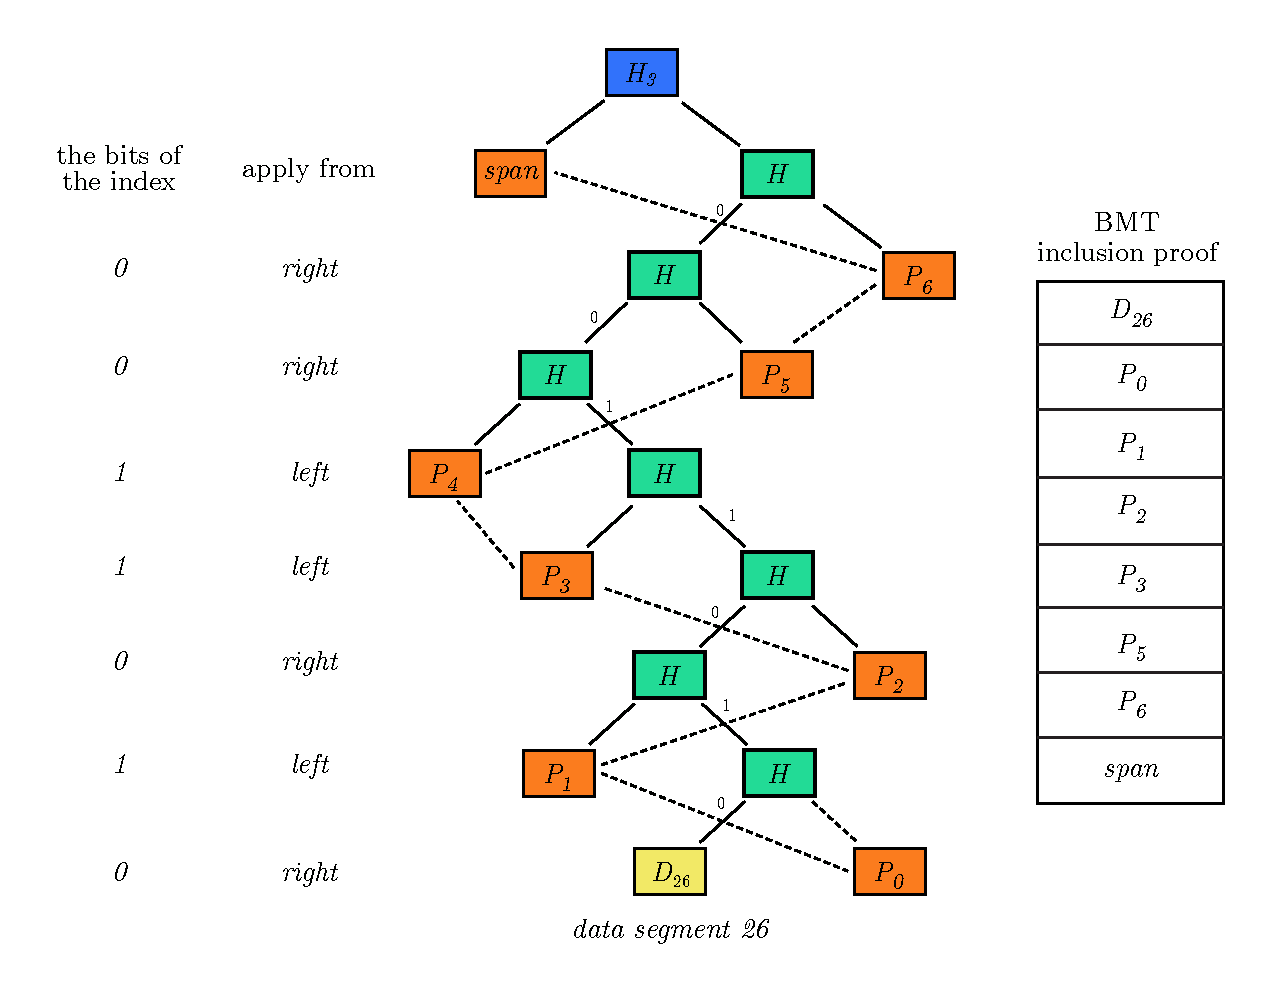
\includegraphics[width=.85\textwidth]{fig/inclusion-proof.pdf}
\caption[Compact segment inclusion proofs for chunks ]{Compact segment inclusion proofs for chunks. Assume we need proof for segment 26 of a chunk (yellow). The orange hashes of the BMT are the sister nodes on the path from the data segment up to the root and constitute what needs to be part of a proof. When these are provided together with the root hash and the segment index, the proof can be verified. The side on which proof item $i$ needs to be applied depends on the $i$-th bit (starting from least significant) of the binary representation of the index. Finally the span is prepended and the resulting hash should match the chunk root hash.}
\label{fig:chunk-inclusion}
\end{figure}

\begin{definition}[BMT segment inclusion proof \statusgreen]
\label{def:sip}
Define  $\proofof{sip}(c,i)$ as the $\mathit{BMT}$ inclusion proof on chunk $c$ for segment index $i$:
%
\begin{eqnarray}
\proofof{sip}&: &\mathit{Chunks}\times \overline{0,127} \mapsto \mathit{SIP}\\
\mathit{SIP}&\defeq&\mathit{Segment}\times\mathit{Segment}^7\times \mathit{byte}\{8\}
\\
\proofof{sip}(c,i) &\defeq &\langle c\idx{\idx{i}},\langle h_0, h_1, \ldots, h_6\rangle, \textsc{metadata}(c)\rangle  
\end{eqnarray}
%
where
%
\begin{eqnarray}
h_j&\defeq& \mathit{BMT}(s_j,j)\\
s_j&\defeq&c\idx{\mathit{start}(i,j)\rangedel\mathit{start}(i,j)+32\cdot 2^j}
\end{eqnarray}
%
where
%
\begin{eqnarray}
\mathit{start}(i,j)&\defeq&
\begin{cases}
0 &\text{if } j=7\\
start(i,j+1) & \text{if } \mathit{int}\left(i / 2^j\right) = 0 \mod 2\\
start(i,j+1)+32\cdot 2^{j} &\text{otherwise}
\end{cases}
\end{eqnarray}
\end{definition}

In order to validate segment inclusion proofs we first introduce the prover hash function $\mathit{H}_{\Pi}$.

\begin{definition}[BMT prover function\statusgreen]
\label{def:prover-function}
%
\begin{eqnarray}
\mathit{H}_{\Pi}&:&\overline{0,127}\times\mathit{SIP}\mapsto\mathit{Address}\\
\mathit{H}_{\Pi}(i,\langle d, sisters, m\rangle)&\defeq&\mathit{H}(m,\mathit{H}_{\Pi}^{\triangle}(7,d,sisters))
\end{eqnarray}
%
where
%
\begin{eqnarray}
\mathit{H}_{\Pi}^{\triangle}&:&\overline{0,7}\times\mathit{Segment}\times\mathit{Segment}^7\mapsto\mathit{Address}\\
\mathit{H}_{\Pi}^{\triangle}(j,d,s)&\defeq& \begin{cases}
d & \text{ if } j=0\\
\mathit{H}(\mathit{H}_{\Pi}^{\triangle}(j-1,d,s)\concat s\idx{j-1}) & \text{if }\mathit{int}(i/2^{j-1}) = 0 \mod 2\\
\mathit{H}(s\idx{j-1}\concat \mathit{H}_{\Pi}^{\triangle}(j-1,d,s)) &\text{otherwise}
\end{cases}
\end{eqnarray}
\end{definition}


\begin{definition}[BMT SIP validation \statusgreen]
\label{def:sip-validation}
Define  $\validator{sip}(a, i, p)$ as the validator of a BMT segment inclusion proof $p$ for chunk at address $a$ on segment index $i$:
%
\begin{eqnarray}
\validator{sip}&:&\mathit{Segment}\times\overline{0,127}\times \mathit{SIP} \mapsto \{\mathtt{T,F}\}
\\
\validator{sip}(a,i,p) &\Leftrightarrow&
\mathit{H}_{\Pi}(i,p)=a
\end{eqnarray}
\end{definition}

\begin{definition}[Single owner chunks data integrity proof \statusgreen]
\label{def:socproof}
Define a single owner chunk storage proof $\proofof{soc}(c,i)$ as a segment inclusion proof of the data payload of SOC $c$ on index $i$ together with the ID and signature of SOC $c$:
%
\begin{eqnarray}
\mathit{SIP}_\mathit{SOC} &\defeq&\mathit{SIP}\times\mathit{Sig}\times\mathit{Segment}\\
\proofof{sip[soc]} &:&\mathit{SOC}\times\overline{0,127}\mapsto\mathit{SIP}_\mathit{SOC}\\ 
\proofof{sip[soc]}(\langle o,id,cac\rangle,i)&\defeq&  \langle p, sig, id\rangle
\end{eqnarray}
%
where
%
\begin{eqnarray}
p&=&\proofof{sip}(cac,i)\\
sig&=&\mathit{Sig}(o,id\concat \mathit{address}(cac))
\end{eqnarray}
\end{definition}

\begin{definition}[Single owner chunks data integrity validation  \statusgreen]
\label{def:socproof-validity}
Define $\validator{sip[soc]}(a, i, p)$ as the validator of a single owner chunk storage proof $p$ for chunk at address $a$ on segment index $i$:
%
\begin{eqnarray}
\validator{sip[soc]}&:&\mathit{Address}\times\overline{0,127}\times\mathit{SIP}_\mathit{SOC}\mapsto\{\texttt{T,F}\}\\ \validator{sip[soc]}(a, i, \langle p, sig, id\rangle)&
\Leftrightarrow&a= \mathit{H}(id\concat o)
\end{eqnarray}
such that 
\begin{eqnarray}
\textsc{owner } o&=& \mathit{ECRecover}(sig,id\concat a')\\
\textsc{payload } a'&=& \mathit{H}_{\Pi}(i,p)
% \\
% \textsc{proof } p&=&\langle d, sisters, m\rangle
\end{eqnarray}
\end{definition}



\subsubsection{Postage stamps}
\begin{definition}[Postage stamps \statusgreen]
\label{def:postage-stamp}
%
\begin{eqnarray}
\mathit{Stamps}&\defeq& \mathit{Segment}\times\mathit{uint64}\times\mathit{Timestamp}\times\mathit{Address}\\
\mathit{ps} &=&\langle  b,i,ts,a\rangle\in \mathit{Stamps} 
\\
\textsc{batchID}(ps) &\defeq& b 
\\
\textsc{index}(ps) &\defeq &i 
\\
\textsc{timestamp}(ps)&\defeq &ts 
\\
\textsc{address}(ps) &\defeq &a 
\end{eqnarray}
\end{definition}


\begin{definition}[Storage slot reference \statusgreen]
\label{def:slot}
Define the \emph{storage slot reference} $\mathit{slot}(ps)$ of a postage stamp $ps$ as the tuple of the batch identifier and the within-batch stamp counter:
%
\begin{eqnarray}
\mathit{Slots}&\defeq&\mathit{Segment}\times\mathit{uint64}\\
\mathit{slot}&:& \mathit{Stamps}\mapsto\mathit{Slots}\\
\mathit{slot}(ps) &\defeq &\langle \textsc{batchID}(ps),\textsc{index}(ps)\rangle 
\end{eqnarray}
%
% Naturally storage slot reference of a chunk $\mathit{slot}(c)$ is defined as the slot reference of the postage stamp attached to the chunk.
\end{definition}


\begin{definition}[Postage stamp validity \statusgreen]
\label{def:postage-stamp-validity}
Define $\validator{stamp}(ps)$ as the validator of the proof of relevance expressed as the postage stamp $ps$ relying on blockchain information:
%
\begin{eqnarray}
\validator{stamp}&:& \mathit{Stamps} \times\Gamma\times\mathit{Nodes}\mapsto \{\mathtt{T,F}\}\\
\validator{stamp}(ps,\gamma,n) &\Leftrightarrow& \\
\textsc{authentic} & & \textsc{batchID}(ps)\in\mathrm{Batches}(\gamma)\wedge
\\
\textsc{alive} & & \mathrm{Balance}(ps) > 0 \wedge 
\\
\textsc{authorised} & &  \mathit{ECRecover}(\mathit{Sig}(ps), \mathit{encode}(ps)) = \mathrm{Owner}(ps) \wedge
\\
\textsc{available} & & 0 <= \textsc{index}(ps) < \mathrm{Size}(ps)\wedge
\\
\textsc{aligned} & & \mathit{PO}(\textsc{index}(ps),n) \geq \textsc{depth}(\mathit{reveal}(\gamma, n))
\end{eqnarray}
\end{definition}

\subsubsection{Ordering and sampling}


\begin{lemma}[Ordering and indexing functions\statusgreen]
\label{lem:ordering}
Given an arbitrary finite set $C$, and another set $I$ with a total order $<$.
Any invertible function total over $C$, $f: C\mapsto I$ defines a total order $<_f$ over $C$ as follows:
%
\begin{eqnarray}
<_f&\subseteq&C\times C\\
\forall c,c'\in C, c<_f c'&\Leftrightarrow& f(c)<f(c')
\end{eqnarray}

\begin{proof}
$f$ is injective wrt $I$, so $\mathit{Image}(f)=J\subseteq I$. Since $<$ restricted to a subset ($<_J$) is also a total order over $J$.
Since $f$ is invertible, $C$ and $J$ are isomorphic and therefore the total order $<$ on $J$ carries over to $C$. \qedsymbol
\end{proof}
\end{lemma}

\begin{corollary}[hash orders\statusgreen]
Any hash function defines a total order on a finite set of byte slices.
%
\begin{proof}
The collision free nature of the hash function makes it practically invertible. The actual hashes when read as binary encodings of integers, offer a natural integer ordering over the values. 
\end{proof}

Example: the prefixed BMT hash transform (see \ref{def:prefixed-hash}) defines a total order over a set of chunks.
\end{corollary}

\begin{definition}[Sampler function]
\label{def:sampler}
%
Using $f$ and its derivative ordering on $C\subseteq\mathit{Dom}(f)$ we represent $C$ as an ordered sequence:
%
\begin{eqnarray}
\overrightarrow{\mathit{Seq}}
&:&(T\mapsto  T)\times\mathcal{P}(T)\mapsto T{*}\\
\overrightarrow{\mathit{Seq}}(f,C) 
&\defeq& C'\\
\text{such that }
f(C'\idx{i})<f(C'\idx{j}) &&\text{ for every } 0\leq i<j<\lvert C\rvert
\end{eqnarray}


Finally, we define a sampler function for any $f$ invertible with an image having a total order and $C\subseteq\mathit{Dom}(f)$ such that it selects a prefix slice of length $l$ from the ordered $C$:         

\begin{eqnarray}
\mathit{Sampler} &:&(T\mapsto  T)\times\mathcal{P}(T)\times \mathit{uint64}\mapsto T{+}\\
% \mathit{Sampler}(f,C) &:&\overline{0,\lvert C\rvert-1}\mapsto T\{,\lvert C\rvert\}\\
\mathit{Sampler}(f,C,l) &\defeq& \overrightarrow{\mathit{Seq}}(f,C)\idx{\rangedel l}
\end{eqnarray}
\end{definition}

\subsection{Redistribution game}\label{sec:appendix-game}
\label{sec:redistribution-game}

\begin{definition}[Redistribution game round\statusgreen]

\label{def:redistribution-game-round} 
Define $\gamma$ as a redistribution game round.  $\gamma$ is conceived of as a multidimensional index:
%
\begin{eqnarray}
\Gamma&\defeq&\mathit{uint64}\times\mathit{uint64}\times\mathit{uint64}\\
\gamma\in\Gamma&=&\langle c,\sigma,i\rangle\\
\textsc{chain}(\gamma)&c&\text{ID of the blockchain context}\\
\textsc{series}(\gamma)&\sigma&\text{index of the parallel series}\\
\textsc{round}(\gamma)&i&\text{sequential index of the round}
\end{eqnarray}

Define $\textsc{block}(\gamma)$ as the starting block height of this particular game $\gamma$:
%
\begin{eqnarray}
\textsc{block}(\gamma)&\defeq&\textsc{round}(\gamma)\cdot \mathtt{ROUND\_LENGTH}+\mathtt{START\_BLOCK}
\end{eqnarray}

Ordering by sequential index defines the chain of games, which lets us define the $\mathit{Prev}$ function:
%
\begin{eqnarray}
\mathit{Prev}&:&\Gamma\mapsto\Gamma\\
\mathit{Prev}(\langle c,\sigma,i\rangle)&\defeq&\langle c,\sigma,i-1\rangle
\end{eqnarray}
\end{definition}

\subsubsection{Transactions and on-chain registers}

The smart contract receives transactions from applicants in phases. The following virtual registers capture the information given in these transactions that are relevant for defining the winner:
\begin{itemize}[noitemsep]
\item[--] batches (see definition \ref{def:postage-stamp-validity})
\item[--] stakes (see definition \ref{def:stakes})
\item[--] commits (see definition \ref{def:commits})
\item[--] reveals (see definition \ref{def:reveals})
\end{itemize}

\begin{definition}[Stakes \statusgreen]
\label{def:stakes}
We define $\mathit{Stakes}$ as the registry of stakes resulting from transactions sent to the staking contract. A record is a tuple of a node overlay, the stake balance and the committed stake and can be updated.  
%
\begin{eqnarray}
\mathit{Stakes}&:&\Gamma\mapsto\mathit{Nodes}\times\mathit{uint64}\times\mathit{uint64}\\
\langle n, s, m\rangle\in\mathit{Stakes}(\gamma)&\Leftrightarrow& \\
\textsc{right age}&&\exists b'<b-\mathtt{MIN\_STAKE\_AGE}, \tau\in\mathrm{Transactions}(b') \\
\textsc{node overlay}&& n = \mathit{H}(\mathrm{origin}(\tau)\concat\mathtt{BZZ\_NETWORK\_ID}\concat\mathrm{data}(\tau)\idx{0})\\
\textsc{stake balance}&& s=\mathrm{amount}(\tau)\\
\textsc{committed stake}&& m=\mathrm{data}(\tau)\idx{1}
\end{eqnarray}
%
There is only one stake allowed per node, so we can define the staked amount belonging to a node as the minumum of the stake balance and the committed stake times the unit price of storage:
% 
\begin{eqnarray}
\mathit{Stake}&:&\Gamma\times\mathit{Nodes}\mapsto\mathit{uint64}\\
\mathit{Stake}(\gamma,n)&\defeq&\mathit{min}(s,m\cdot \mathit{Price}(\gamma))
\end{eqnarray}
%
\end{definition}

\begin{definition}[Commits \statusgreen]
\label{def:commits}
We define $\mathit{Commits}(\gamma)$ as the registry of applications for a game $\gamma$ resulting from a transaction sent to the game contract's \emph{commit} endpoint. A tuple of the overlay of the committing node, its commitment hash and the number of the block containing the transaction is entered in the register after verifying that (i) the transaction was sent during the commit phase (right time), and (ii) that the node has enough stake and is not frozen (right amount).                    
%
\begin{eqnarray}
\mathit{Commits}&:&\Gamma\mapsto\mathit{Nodes}\times\mathit{Segment}\times\mathit{Blocks}\\
\langle n,h,b\rangle\in\mathit{Commits}(\gamma)&\Leftrightarrow&%\text{$n$ submitted $h$ as their commit}
\\
% &&\text{during the commit phase}\\
\textsc{right time}
&&b < \mathtt{PHASE\_LENGTH} \mod \mathtt{ROUND\_LENGTH} \\
\textsc{right amount}&&\mathit{stake}(\gamma,n)\geq \texttt{MINIMUM\_STAKE}\\
(\textsc{redundancy})&&
\end{eqnarray}
\end{definition}

\begin{definition}[Reveals\statusgreen]
\label{def:reveals}
We define $\mathit{Reveals}$ as the registry of reveals resulting from a transaction sent to the game contract's reveal endpoint. The reveal record is a tuple of the node overlay, the two commitment hashes, the self-reported storage depth, a serial index used for sorting, the obfuscation key, and the block number. The record is entered in the register after it is validated that (i) it was submitted during the reveal phase (right time), (ii) the commitments when obfuscated match the commit by the same node (right reveal), and (iii) that the neighbourhood selection anchor falls within the node's area of responsibility using the self-reported depth (right location). 
%
\begin{eqnarray}
\mathit{RevealEntry}&:&\mathit{Nodes}\times\mathit{Address}^2\times\mathit{uint8}^2\times\mathit{Nonce}\times\mathit{Blocks}\\
\mathit{Reveals}&:&\Gamma\mapsto\mathcal{P}(\mathit{RevealEntry})\\
r=\langle n,chc,chs,sd,i,k,b\rangle\in\mathit{Reveals}(\gamma)&\Leftrightarrow& 
% \text{ $n$ reveals $chc, chs, sd$  as their commitment}\\
\langle\\
\textsc{node}(r)&=&n\\
\textsc{chc}(r)&=&chc\\
\textsc{chs}(r)&=&chs\\
\textsc{depth}(r)&=&sd\\
\textsc{index}(r)&=&i\\
\textsc{nonce}(r)&=&k\\
\textsc{block}(r)&=&b\\
&&\rangle\\
&\Leftrightarrow&\\
\textsc{right time}
&&p \leq b < 2p \mod r\\
&& p = \mathtt{PHASE\_LENGTH}, r= \mathtt{ROUND\_LENGTH} \\
\textsc{right reveal}&&\mathit{H}(n\concat sd\concat chc\concat chs\concat k)=h \text{ such that }\\
&&\langle n,h,b'\rangle\in\mathit{Commits}(\gamma)\text{ for some }b'\\
\textsc{right location}&&\mathit{PO}(\mathit{addr}(n),\mathit{NSA}(\mathit{Prev}(\gamma)))\geq sd\\
(\textsc{responsibility})&&
\end{eqnarray}
%
There is only one reveal allowed per node, so we can define the reveal belonging to a node:
%
\begin{eqnarray}
\mathit{Reveal}&:&\Gamma\times\mathit{Nodes}\mapsto\mathit{RevealEntry}\\
\mathit{Reveal}(\gamma, n)&=&r
\end{eqnarray}
such that 
\begin{eqnarray}
n&=&\mathit{Node}(r)\\
r&\in&\mathit{Reveals}(\gamma)
\end{eqnarray}
\end{definition}

\subsubsection{Random nonces}

\begin{definition}[Random nonces for the round\statusgreen]
\label{def:nonce-round}

From the round's random seed (see definition \ref{def:random-seed} appendix \ref{sec:randomness}) we can derive all the necessary random input nonces:
%
\begin{eqnarray}
\textsc{ N.hood Selection Anchor   }\mathit{NSA}(\gamma)&\defeq&\mathit{H}(\mathcal{R}(\gamma)\concat BE^{64}(\mathit{SK}(\gamma)))\\
\textsc{ Truth Selection Nonces  }\mathit{TSN}(\gamma)&\defeq&\mathit{H}(\mathcal{R}(\gamma)\concat\mathit{BE}^{8}(0)) \\
\textsc{ Winner Selection Nonces  }\mathit{WSN}(\gamma, i)&\defeq&\mathit{H}(\mathcal{R}(\gamma)\concat\mathit{BE}^{8}(1)) \\
\textsc{ Reserve sampling salt } \mathit{RSS}(\gamma)&\defeq&\mathit{H}(\mathcal{R}(\gamma)) \\
\textsc{ Segment Selection Nonce } \mathit{SSN}(\gamma,i)&\defeq&\mathit{H}(\mathcal{R}(\gamma)\concat\mathit{BE}^{8}(i))
\end{eqnarray}
where 
\begin{eqnarray}
\mathit{SK}&:&\Gamma\mapsto\mathit{uint64}\\
\mathit{SK}(\gamma)&\defeq&\begin{cases}0&\text{if }\lvert\mathit{Reveals}(\gamma)\rvert>0\\
\mathit{SK}(\mathit{Prev}(\gamma))+1&\text{otherwise}
\end{cases}
\end{eqnarray}

Let us now define the witness selection function $\mathcal{W}$ that selects two random witness indexes as well as the last index of the reserve sample such that they are all distinct:
%
\begin{eqnarray}
\mathcal{W}&:&\Gamma\times\mathit{uint64}\times\{0,1,2\}\mapsto\mathit{uint8}\\
\mathcal{W}(\gamma,m,k)&\defeq&\begin{cases}
\mathit{SSN}(\gamma,0) \mod m-1&\text{ if }k=0\\
m-1&\text{ if }k=2\\
m-2&\text{ if }k=1 \land\\
& \mathit{SSN}(\gamma,0)=\mathit{SSN}(\gamma,1) \mod m-1\\
\mathit{SSN}(\gamma,1) \mod m-2&\text{ otherwise }
\end{cases}
\end{eqnarray}
\end{definition}

% \subsubsection{Reserve Size}

% \begin{definition}[Network reserve size]
% \label{def:reserve-size}
% Define $\mathrm{ReserveSize}(\gamma)$, the network reserved capacity as the total number of storage slots by all batches valid at block $\mathit{Block}(\gamma)$. This can be read from the batch registry contract:
% %
% \begin{eqnarray}
% \mathrm{ReserveSize}&:&\Gamma\mapsto \mathit{uint64}\\
% \mathrm{ReserveSize}(\gamma)&\defeq&\Sigma_{b\in \mathit{Batches}(\gamma)}\mathrm{Size}(b,\gamma)
% \end{eqnarray}
% \end{definition}


% \begin{definition}[Reserve depth]
% \label{def:reserve-depth}
% Define $\mathrm{ReserveDepth}(\gamma)$ as the base 2 log of the number of neighbourhoods needed to provide redundant storage for the volume of chunks corresponding to the network reserve size at block $\mathit{Block}(\gamma)$ given a fixed node storage capacity of depth \texttt{NODE\_RESERVE\_DEPTH}:
% %
% \begin{eqnarray}
% \mathrm{ReserveDepth}&:&\Gamma\mapsto \mathit{uint8}\\
% \mathrm{ReserveDepth}(\gamma)&\defeq&\mathit{int}(\mathit{log}_2(\mathrm{ReserveSize}(\gamma)))-\texttt{NODE\_RESERVE\_DEPTH}
% \end{eqnarray}
% \end{definition}


\subsubsection{Winner selection and claim validation}

\begin{definition}[Prefixed hash \statusgreen]
\label{def:prefixed-hash}
Define the hash prefixing function $\mathit{prefix}(H,p)$ as a function which when applied to a hash function $\mathit{H}$ and a constant byte slice $p$  outputs a hash function which for every input returns the hash of the input prefixed by $p$ using $H$.
%
\begin{eqnarray}
\mathit{prefix}&: &(\mathit{byte}{*}\mapsto\mathit{Segment})\times\mathit{byte}{*}\mapsto (\mathit{byte}{*}\mapsto\mathit{Segment})
\\
\mathit{prefix}(H,p) &: &\mathit{byte}{*}\mapsto\mathit{Segment}\\
\mathit{prefix}(H,p)(b) &\defeq & H(p\concat b)
\end{eqnarray}

Exceptionally, we define the prefixed version of BMT hash (denoted as $\mathit{BMT}[]$) as one   that uses the prefixed verson of its base hash:
%   
\begin{eqnarray}
\mathit{BMT}[]&: &\mathit{byte}{*}\mapsto\mathit{Chunk}\times\mathit{byte}\{8\}\mapsto\mathit{Segment}\\
\mathit{BMT}[p]&\defeq&\mathit{BMT}[\mathit{prefix}(\mathit{H},p)]
\end{eqnarray}

\end{definition}
    
\begin{definition}[Transformed chunk reserve sample\statusgreen]
\label{def:transformed-reserve}
%
Let us now define the chunk transformation function $\Delta^C(p)$
for a random nonce prefix $p$ as follows: 
%
\begin{eqnarray}
\Delta^C&:&\mathit{Nonce}\mapsto\mathit{Chunks}\mapsto\mathit{Segment}\\
\Delta^C(p)&:&\mathit{Chunks}\mapsto\mathit{Segment}\\
\Delta^C(p)(c)&\defeq&\mathit{BMT}[p](\textsc{data}(c),\textsc{metadata}(c))
\end{eqnarray}
%
Define the transformed reserve sample $\mathit{RS^C}(\gamma,n)$ for game $\gamma$ and node $n$ as the first  $2^d$ chunks of the node's reserve at block $\textsc{block}(\gamma)$, using the ordering defined (see lemma \ref{lem:ordering} and definition \ref{def:sampler}) by the hash (see definition \ref{def:prefixed-hash}) of their data  using BMT with 256-bit Keccak prefixed with random nonce $p$ as its base hash.
%
\begin{eqnarray}
\mathit{RS^C}&:&\Gamma\times\mathit{Nodes}\mapsto\mathit{Chunks}{*}\\\
\mathit{RS^C}(\gamma,n)&\defeq&\mathit{Sampler}(\Delta^C(p),\mathit{Reserve}(\gamma,n),2^d)
\end{eqnarray}
where 
\begin{eqnarray}
d & = & \texttt{SAMPLE\_DEPTH} \text{ (see \ref{sec:constants})} \\
p & = & \mathit{RSS}(\gamma) \text{ (see definition \ref{def:nonce-round})}
\end{eqnarray}
\end{definition}


\begin{definition}[Chunk reserve sample commitment hash \statusgreen]
\label{def:chc}
Define $\mathit{CH^C}(\gamma,n,)$ for game $\gamma$ and node $n$ as the BMT chunk hash of the packed address chunk (see definition \ref{def:pac}) packing the chunks of the transformed reserve sample (see definition \ref{def:transformed-reserve}) for game $\gamma$ and node $n$.
%
\begin{eqnarray}
\mathit{CH^C}&:&\Gamma\times\mathit{Nodes}\mapsto\mathit{Address}\\
\mathit{CH^C}(\gamma,n)&\defeq&\mathit{Address}(\mathit{PAC^C}(\mathit{RS^C}(\gamma, n)), p)
    \end{eqnarray}
where
\begin{eqnarray}
p & = & \mathit{RSS}(\gamma) \text{ (see definition \ref{def:nonce-round})}
\end{eqnarray}
and where 
\begin{eqnarray}
\mathit{PAC^C}&:&\mathit{Chunks}{*}\times\mathit{Nonce}\mapsto\mathit{Chunks}\\
\mathit{PAC^C}(C,p)&\defeq&\mathit{CAC}{}\left(\Concat_{i=0}^{\mathit{len}(C)-1} \mathit{Seg}(C\idx{i},p), m\right)
\end{eqnarray}
where
\begin{eqnarray}
\mathit{Seg}(C\idx{i},p) &=& \mathit{Address}(C\idx{i})\concat \Delta^C(p)(C\idx{i}) \\
m & = & \mathit{LE}^{64}(2\cdot32\cdot\mathit{len}(C))
\end{eqnarray}
\end{definition}

\begin{definition}[Transformed slots reserve sample\statusgreen]
\label{def:transformed-slots}
%
Let us now define the slots transformation function $\Delta^S(p)$
for a random nonce $p$ as follows: 
%
\begin{eqnarray}
\Delta^S&:&\mathit{Nonce}\mapsto\mathit{Chunks}\mapsto\mathit{Segment}\\
\Delta^S(p)&:&\mathit{Chunks}\mapsto\mathit{Segment}\\
\Delta^S(p)(c)&\defeq&\mathit{H}[p](\mathit{Slot}(\mathit{Stamp}(c)))
\end{eqnarray}
%
Define the transformed reserve sample $\mathit{RS^S}(\gamma,n)$ for game $\gamma$ and node $n$ as the first $2^d$ chunks  of the node's reserve at block $\textsc{block}(\gamma)$, using the ordering defined by the slot transformation function using prefix $p$:%
\begin{eqnarray}
\mathit{RS^S}&:&\Gamma\times\mathit{Nodes}\mapsto\mathit{Chunks}{*}\\\
\mathit{RS^S}(\gamma,n)&\defeq&\mathit{Sampler}(\Delta^S(p),\mathit{Reserve}(\gamma,n),2^d)
\end{eqnarray}
where 
\begin{eqnarray}
d & = & \texttt{SAMPLE\_DEPTH} \text{ (see \ref{sec:constants})} \\
p & = & \mathit{RSS}(\gamma) \text{ (see definition \ref{def:nonce-round})}
\end{eqnarray}
\end{definition}


\begin{definition}[Transformed slots reserve sample commitment hash \statusgreen]
\label{def:chs}
Define $\mathit{CH^S}(\gamma,n)$ for game $\gamma$ and node $n$ as the BMT chunk hash of the packed address chunk (see definition \ref{def:pac}) the chunks of the transformed reserve sample (see definition \ref{def:transformed-reserve}) for game $\gamma$ and node $n$.
%
\begin{eqnarray}
\mathit{CH^S}&:&\Gamma\times\mathit{Nodes}\mapsto\mathit{Address}\\
\mathit{CH^S}(\gamma,n)&\defeq&\mathit{Address}(\mathit{PAC}(\mathit{RS^S}(\gamma, n),m))
\end{eqnarray}
where
\begin{eqnarray}
m & = & \mathit{LE}^{64}(32\cdot 2^d)\\
d & = & \texttt{SAMPLE\_DEPTH} \text{ (see \ref{sec:constants})} 
\end{eqnarray}
\end{definition}

\begin{definition}[Weighted selection\statusgreen]
\label{def:weighted-selection}
We define $\mathit{WeightedSelect}(w,k)$ as a sampler function which selects an index $0<i<\mathit{len}(w)$ such that the indexes have a probability of being selected according to the weights in $w$ determined by the input nonce (pseudorandom number) $k$.
%
\begin{eqnarray}
\mathit{WeightedSelect}&:&\mathit{uint256}{+}\times\mathit{uint256}\mapsto\mathit{uint256}{+}\\
\mathit{WeightedSelect}(w,k)&\defeq&
\begin{cases}
    i&\text{if }k <w\idx{i}\mod W\idx{i}\\
\mathit{WeightedSelect}(w\idx{\rangedel i},k)&
\text{otherwise}
\end{cases}
\end{eqnarray}
such that $i=\mathit{len}(w)-1$,   
and
where $W$ (cumulative weights) is defined as
\begin{eqnarray}
W & : & \mathit{uint256}{+}\mapsto\mathit{uint256}\\
W\idx{i} &\defeq & \begin{cases}
    w\idx{0}&\text{if }i=0\\
    W\idx{i-1}+w\idx{i}&\text{otherwise}
\end{cases} 
\end{eqnarray}
\end{definition}



\begin{definition}[Truth selection\statusgreen]
\label{def:truth-selection}
We determine the truth from reveals through selection weighted by stake density using the truth selection nonce as random input. 
\begin{eqnarray}
\mathit{Truth}&:& \Gamma\mapsto\mathit{RevealEntry}\\
\mathit{Truth}(\gamma)&\defeq&\mathit{R}(\gamma)\idx{\mathit{WeightedSelect}(\mathit{weights},\mathit{TSN}(\gamma))}
\end{eqnarray}
where weights are stake densities such that 
\begin{eqnarray}
\mathit{weights}\idx{i}&=&\mathit{Stake}(\gamma,\textsc{node}(R\idx{i}))\cdot 2^{\textsc{depth}(R\idx{i})}
\end{eqnarray}
where $R$ is the reveals of the round sorted by index:
\begin{eqnarray}
R&=&\overrightarrow{\mathit{Seq}}(\textsc{index},\mathit{Reveals}(\gamma))
\end{eqnarray}
\end{definition}

\begin{definition}[Honest reveals\statusgreen]
We define honest reveals as the subset of reveals for the round agreeing with the truth in reserve commitment hashes and storage depth.
\label{def:honest-reveals}
\begin{eqnarray}
\mathit{HonestReveals}&:&\Gamma\mapsto\mathit{RevealEntry}{*}\\
\mathit{HonestReveals}(\gamma)&\defeq&\overrightarrow{\mathit{Seq}}(\textsc{index},\{r\in\mathit{Reveals}(\gamma)|\mathit{Honest}(r)\})
\end{eqnarray}
where
\begin{eqnarray}
\mathit{Honest}&:&\mathit{RevealEntry}\mapsto\{\texttt{T,F}\}\\
\mathit{Honest}(r)&\leftrightarrow&\\
&&\textsc{chc}(r)=\textsc{chc}(\mathit{truth}(\gamma))\ \land\\
&&\textsc{chs}(r)=\textsc{chs}(\mathit{truth}(\gamma))\ \land\\
&&\textsc{depth}(r)=\textsc{depth}(\mathit{truth}(\gamma))
\end{eqnarray}
\end{definition}

\begin{definition}[Winner selection\statusgreen]
\label{def:winner-selection}
We determine the winner from honest reveals through selection weighted by stake using the winner selection nonce as random input. 
\begin{eqnarray}
\mathit{Winner}&:& \Gamma\mapsto\mathit{RevealEntry}\\
\mathit{Winner}(\gamma)&\defeq&\mathit{HonestReveals}(\gamma)\idx{\mathit{WeightedSelect}(\mathit{weights},\mathit{WSN}(\gamma))}
\end{eqnarray}
where weights are stakes such that 
\begin{eqnarray}
\mathit{weights}\idx{i}&=&\mathit{Stake}(\gamma,\textsc{node}(\mathit{HonestReveals}\idx{i}))
\end{eqnarray}
\end{definition}

\subsubsection{Proofs of reserve}
\label{sec:proofs}
    
\begin{definition}[Proof of reserve \statusgreen]
\label{def:por}
Proof of reserve provides evidence that the reserve is replicating relevant content and shows a proof of recency of retaining chunk data in full integrity.
%
\begin{eqnarray}
\mathit{POR}&:&\mathit{SIP}^2\times\mathit{Stamps}\\
\proofof{r}&:&\Gamma\times\mathit{Chunks}\times\mathit{Chunks}{+}\times\{0,1,2\}\mapsto\mathit{POR}\\
\proofof{r}(\gamma,c,C,k)&\defeq&\langle\\
\textsc{witness proof}&&\proofof{sip}(c,d\cdot i), \\
\textsc{retention proof}&&\proofof{sip}(C\idx{i},j), \\
\textsc{postage stamp}&&\mathit{Stamp}(C\idx{i})\\
&&\rangle
\end{eqnarray}
where 
\begin{eqnarray}
i&=&\mathcal{W}(\gamma,\mathit{len}(C),k)\\
j&=& \mathit{SSN}(\gamma,k)\mod 128\\
d &=&\frac{\mathit{SegCnt}(c)}{\mathit{len}(C)} \left(=\begin{cases}
    1& \text{if } C=RS^S\\
2 &\text{if } C=RS^C
\end{cases}
\right)
\end{eqnarray}
\end{definition}


\begin{definition}[Proof of reserve validation\statusgreen]
\label{def:por-validation}
%
\begin{eqnarray}
\validator{r}&:&\Gamma\times\mathit{Nodes}\times\mathit{Address}\times\{0,1,2\}\times\mathit{POR}\mapsto\{\texttt{T,F}\}\\
\validator{r}(\gamma, n, ch, k, \pi)&\leftrightarrow& \\
\textsc{relevance}&&\validator{sip}(ch,d\cdot i,p_w)\land\\
    && \validator{stamp}(ps, \gamma, n) \land\\
\textsc{retention}&& \textsc{data}(p_w)=a\land\\
    && \validator{sip}(a,j,p_r)\land\\
\textsc{recency}&&i=\mathcal{W}(\gamma,\mathit{SegCnt}(p_w),k)\land\\
    &&j = \mathit{SSN}(\gamma,k)\mod 128\land\\
\textsc{retrievability}&&\mathit{PO}(a,n) \geq sd 
\end{eqnarray}
where
\begin{eqnarray}
a&=& \textsc{Address}(ps)\\
\pi&=&\langle p_w, p_r, ps\rangle\\
sd &=& \textsc{depth}(\mathit{Reveal}(\gamma, n))\\
d&=&\frac{\mathit{SegCnt}(p_w)}{2^D}\left(=\begin{cases}
    1& \text{if } C=RS^S\\
2 &\text{if } C=RS^C
\end{cases}\right)\\
D& =& \texttt{SAMPLE\_DEPTH} \text{ (see \ref{sec:constants})}
\end{eqnarray}
\end{definition}


\begin{definition}[Proof of chunk density validation\statusgreen]
\label{def:chunk-density-validition}
%
Define $\validator{cd}(\gamma, p_0,p_1,p_2)$ as the validation function for the proof of chunk density for round $\gamma$ and proof of reserve and segment inclusion proof pairs $p_0,p_1,p_2$.
%
\begin{eqnarray}
\mathit{PORT}&:&\mathit{POR}\times\mathit{SIP}\\
\validator{cd}&:&\Gamma\times\mathit{PORT}^3\mapsto\{\texttt{T,F}\}\\
\validator{cd}(\gamma, \pi_0,\pi_1,\pi_2)&\leftrightarrow&\\
\textsc{right data segment}&&   \textsc{data}(pr_k)= \textsc{data}(pt_k)\text{ for }k\in\{0,1,2\}\land\\
\textsc{right address}&& \textsc{sister}(pw_k,0)=ta_k\text{ for }k\in\{0,1,2\}\land\\
\textsc{right order}&& ta_0<ta_1<ta_2\land\\
\textsc{right size}&& ta_2\leq\texttt{MAX\_SAMPLE\_VALUE}
\end{eqnarray}
where  for $k\in\{0,1,2\}$
\begin{eqnarray}
ta_k& = & \mathit{H}_{\Pi}(p,j_k,pt_k)\\
j_k& = &\mathit{SSN}(\gamma,k)\mod 128\\
\pi_k&=& \langle\langle pw_k, pr_k, \_\rangle, pt_k\rangle
% \\
% w_k&=&\langle O+i_k,ta_k\rangle
\end{eqnarray}
and where
\begin{eqnarray}
p & = & \mathit{RSS}(\mathit{Prev}(\gamma)) \text{ (see definition \ref{def:nonce-round})}
% D& =& \texttt{NODE\_RESERVE\_DEPTH} \text{ (see \ref{sec:constants})}
\end{eqnarray}
\end{definition}

\begin{definition}[Proof of stamp density validation\statusgreen]
\label{def:stamp-density-validition}
%
Define $\validator{sd}(\gamma, ps_0,ps_1,ps_2)$ as the validation function for the proof of stamp density for round $\gamma$ and postage stamps $ps_0,ps_1,ps_2$.
%
\begin{eqnarray}
\validator{sd}&:&\Gamma\times\mathit{Stamps}^3\mapsto\{\texttt{T,F}\}\\
\validator{sd}(\gamma, ps_0,ps_1,ps_2)&\leftrightarrow &\\ 
\textsc{right order}&& ta_0<ta_1<ta_2\land\\
\textsc{right size}&& ta_2\leq\texttt{MAX\_SAMPLE\_VALUE}
\end{eqnarray}
where for $k\in\{0,1,2\}$
\begin{eqnarray}
ta_k& =& \mathit{H}(\mathit{Slot}(ps_k)\concat p)
\end{eqnarray}
and where
\begin{eqnarray}
p & = & \mathit{RSS}(\mathit{Prev}(\gamma)) \text{ (see definition \ref{def:nonce-round})}
\end{eqnarray}
\end{definition}

% \newpage
\begin{definition}[Proof of entitlement\statusgreen]
\label{def:poe}
Proof of entitlement captures all the evidence a node needs to submit with their claim transaction to valildate. 
%
\begin{eqnarray}
\mathit{POE}&:&\mathit{PORT}^3\times\mathit{POR}^3\\
\proofof{ent}&:&\Gamma\times\mathit{Nodes}\mapsto\mathit{POE}\\
\proofof{ent}(\gamma,n)&\defeq&\langle\\
&&\langle\proofof{por}(\gamma,n,\mathit{PAC^C}(crs,p), crs,0),pt_0\rangle,\\
&&\langle\proofof{por}(\gamma,n,\mathit{PAC^C}(crs,p),crs,1),pt_1\rangle,\\
&&\langle\proofof{por}(\gamma,n,\mathit{PAC^C}(crs,p),crs,2),pt_2\rangle,\\
&&\proofof{por}(\gamma,n,\mathit{PAC}(srs),srs,0),\\
&&\proofof{por}(\gamma,n,\mathit{PAC}(srs),srs,1),\\
&&\proofof{por}(\gamma,n,\mathit{PAC}(srs),srs,2),\\
&&\rangle
\end{eqnarray}
where for $k\in\{0,1,2\}$
\begin{eqnarray}
pt_k&=& {\proofof{sip}_\mathit{prefix}}(p,r\idx{i_k},j_k)\\
j_k & = & \mathit{SSN}(\gamma,k)\mod 128\\
i_k & = & \mathcal{W}(\gamma,\mathit{length}(crs),k)
\end{eqnarray}
and where 
\begin{eqnarray}
crs& = & \mathit{RS^C}(\gamma, n)\\
srs & = & \mathit{RS^S}(\gamma, n)\\
p & = & \mathit{RSS}(\mathit{Prev}(\gamma)) \text{ (see definition \ref{def:nonce-round})}
\end{eqnarray}
\end{definition}




\begin{definition}[Winner's claim validation\statusgreen]
\label{def:claim-validation}
%
Define $\validator{poe}(\gamma, p)$ as the validation function for the proof of entitlement $p$ as part of the winning claim for game $\gamma$:
%
\begin{eqnarray}
\validator{poe}&:&\Gamma\times\mathit{POE}\mapsto\{\texttt{T,F}\}\\
\validator{poe}(\gamma, p) &\Leftrightarrow\\
%
\textsc{reserve:\ \ \ \ \ \ \ \ \ \ \ \ \ \ }\\
\textsc{chunks}
&&\forall k\in\{0,1,2\},\validator{r}(\gamma,n,\textsc{chc}(r),k,\pi_k)\land\\
\textsc{stamps}
&&\forall k\in\{0,1,2\}, \validator{r}(\gamma,n,\textsc{chs}(r),k,\phi_k)\land\\
\textsc{reserve size:\ \ \ \ \ \ \ }\\
\textsc{chunk density}&&\validator{cd}(\gamma, \langle \pi_0,pt_0\rangle, \langle \pi_1,pt_1\rangle, \langle \pi_2,pt_2\rangle)\land\\
%
\textsc{stamp density}&&
\validator{sd}(\gamma,\textsc{ps}(\phi_0),\textsc{ps}(\phi_1),\textsc{ps}(\phi_2))
\end{eqnarray}
where
\begin{eqnarray}
n&=& \textsc{node}(r)\\
r&=& \mathit{Winner}(\gamma)\\
p &= &\langle\langle \pi_0,pt_0\rangle, \langle \pi_1,pt_1\rangle,\langle \pi_2,pt_2\rangle,\phi_0,\phi_1,\phi_2\rangle
\end{eqnarray}
\end{definition}

% \textsc{redundancy}&& \mathit{Stake}(\gamma, n)\geq \texttt{MINIMUM\_STAKE} \land\\
% \textsc{responsibility}&& \mathit{PO}(\mathit{addr}(n),\mathit{NSA}(\gamma))\geq sd \land\\


\begin{corollary}[Outpayment scheme is fair]
Rewarding the pot to randomly selected neighbourhood implements a  redistribution scheme that is fair across neighbourhoods.
\begin{proof}
With the consensus mechanism we can show that the Nash-optimal strategy of nodes is to follow the protocol and consent on the reserve. On the other hand, the optimal strategy for uploaders is to uniformly distribute chunks across the name space. As a consequence, nodes are expected to have identical storage depth and its variance is independent of being chosen. Long term then relative cumulative outpayments by the redistribution game converge to the fair share.
\end{proof}

Secondly, we argue that the mode of selecting the winner is fair within neighbourhoods. 
\begin{proof}
    
\end{proof}
\end{corollary}


\subsection{Price oracle}
\label{sec:appendix-price-oracle}

The price oracle smart contract receives input from the  redistribution game. Notably the input constitutes information on storage supply relative to the current demand. Since demand is maxed out with storage depth, this information is simply captured by the number of honest revealers per neighbourhood. Rounds when there are no revealers should be treated as rounds where the number of revealers is zero therefore the number of skipped rounds is passed to the price update function too.

\begin{definition}[price function \statusgreen]
\label{def:price-update-function}
The $\mathit{Price}$ function determines the unit price of storage (PLUR/chunk/block). It is defined in such a way that the ratio between the price of rent in consecutive rounds is an exponential function of supply. Supply is the deviation from the optimal number of peers in a neighbourhood as measured by the number of honest revealers in the previous round. 
\begin{eqnarray}
\mathit{Price}&:&\Gamma\mapsto\mathit{uint256}\\
\mathit{Price}(\gamma) &\defeq&\mathit{Price}(\mathit{Prev}(\gamma))\cdot 2^{\sigma\cdot d}
\end{eqnarray}
where
\begin{eqnarray}
\textsc{supply} && d = \texttt{NHOOD\_PEER\_COUNT}-\lvert\mathit{Reveals}(\gamma)\rvert\\
\textsc{reactivity} && \sigma = \frac{1}{\texttt{PRICE\_2X\_ROUNDS}}
\end{eqnarray}
First, note that for a consistent deviation signal $d$, the price change after $n$ rounds is given by multiplying the starting price with $\left(2^{\sigma\cdot d}\right)^n$. The price has doubled if this expression is $2$, i.e., $n\cdot d\cdot \sigma =1$.  
With the lowest signal of undersupply ($r=3$), $d=1$, and therefore the reactivity parameter is expressed as $\sigma=\frac{1}{n}$. In other words $\frac{1}{\sigma}$ measures the number of rounds it takes for the price to double.
\end{definition}


% The price oracle simply applies a price update function which calculates the price of the new round by multiplying the previous rounds's price with the \emph{price update coefficient}. 

% \begin{definition}[price update coefficient \statusgreen]
% \label{def:price-update-coefficient}
% \end{definition}
\subsection{Parameter constants \statusgreen}
\label{sec:constants}

% \subsubsection*{}
Table \ref{tab:constants} 
lists the constants used by Swarm with their type, default value and description.
% {\small 

\begin{longtable}{l|l|p{.07\textwidth}|p{.45\textwidth}}
\toprule
\textsc{constant name}&\textsc{type}&\textsc{value}&\textsc{description}\\\midrule
\texttt{BZZ\_NETWORK\_ID} & \textit{uint64} & 0 & ID of the swarm network
\\
\texttt{PHASE\_LENGTH} & \textit{uint64} &  38& length of commit phase of the redistribution game round in number of blocks
\\
\texttt{ROUND\_LENGTH} & \textit{uint64} & 152 & length of one redistribution game round in number of blocks, fixed at $4$ times the $\mathtt{PHASE\_LENGTH}$
\\
\texttt{NODE\_RESERVE\_DEPTH} & \textit{uint8}&  23 & size requirement for client reserve capacity given in log number of chunks                               
\\
\texttt{SAMPLE\_DEPTH} & \textit{uint8} & 4 & base 2 log number of chunks in sample
\\
\texttt{MAX\_SAMPLE\_VALUE} & \textit{uint256} & $1.2844e+72$ & maximum value for last transformed address in reserve sample, i.e., $<{}1\%$ chance the sampled set size is below a fourth of the prescribed node reserve size.
\\  
\texttt{MINIMUM\_STAKE} & \textit{uint256} & 10 & minimum stake amount in BZZ to be redefined as minimum stake given in storage rent units
\\
\texttt{MIN\_STAKE\_AGE} & \textit{uint256} & 228 & minimum number of blocks stakers need to wait after update or creation for the stake to be useable. Defaults to one and a half rounds to prevent opportunistic manipulation of stake after a neighbourhood is selected.
\\% \texttt{PRICE\_SIGNAL\_COEFF} & \textit{uint64} &  & 
% \\
\texttt{PRICE\_2X\_ROUNDS} & \textit{uint64} & 64 & number of rounds it takes for the price to double in the presence of a consistent lowest degree signal of undersupply.
\\
\texttt{NHOOD\_PEER\_COUNT} & \textit{uint8} & 4 & minimum number of nodes required to form a fully connected neighbourhood.
\\\bottomrule
\caption{Parameter constants}
\label{tab:constants}
\end{longtable}



\section{Source of randomness}\label{sec:randomness}

As the \emph{neighbourhood selection anchor} will directly affect which neighbourhood wins the pot, it is prudent to derive the randomness from a source of entropy that cannot be manipulated. A common solution to obtain randomness is to have independent parties committing to a random nonce with a stake. The random seed for a round is defined as the xor of all revealed nonces. Given the nonces are independent sources fixed in the commit, no individual participant has the ability to skew randomness by selecting a particular nonce. Thanks to the commutativity of xor, the order of reveals is also irrelevant. However, if the reveal transactions are sequential, committers compete at holding out since the last one to reveal can effectively choose the resulting seed to be either including its committed nonce (if they do reveal) or not (if they do not reveal). The threat to slash the stake of non-revealers serves to eliminate this degree of freedom from last revealers and thus renders this scheme a secure random oracle assuming there is at least one honest (non-colluding) party.%
%
\footnote{If the stake is higher than the reward pot, one cannot  afford being slashed with even just one commit without a loss. If this cannot be guaranteed, slashing of the stake is not an effective deterrent.}

Now note that the redistribution scheme already has a commit reveal scheme as well as stake slashed for non-revealers, so a potential random oracle is already part of the proposed scheme. Incidentally, the beginning of the claim phase is when new randomness is needed to select the truth and a winner. Importantly, these random values are only needed if there is a claim which implies that there were some commits and reveals to choose from. Or conversely, if there are no reveals in the round,%
%
\footnote{If saboteurs get slashed or frozen in the claim transaction, if there is no claim, the committers get away without being punished. This can be remedied if the staking contract keeps a flag on each overlay (set when commits, unsets when reveals in the same round) and the check and punishment happens as a result of a commit call in the case the flag is found set.}
%
the random seed is undefined but is also not needed for the claim.

The random seed that transpires at the beginning of the claim phase can serve as the \emph{reserve sample salt} (nonce input to modified hash used in the sampling) with which the nodes in the selected neighbourhood can start calculating their reserve sample. 

The neighbourhood for the next round is selected by the \emph{neighbourhood selection anchor}, which is, similarly to the truth and winner selection nonces, deterministically derived from the same random seed. Unlike the nonces used to select from the reveals, neighbourhood selection should be well defined for the following round even if a round is skipped, i.e., when there is no reveals. To cover this case skipped rounds keep the random seed of the previous round. However, in order to rotate selected neighbourhoods through skipped rounds, we derive the neighbourhood selection anchor from the seed by factoring in the  number of game rounds passed since the last reveal.%
%
\footnote{Otherwise a selected neighbourhood could collude maliciously not to commit/reveal and have the pot roll over to the following round. By simply holding out for a number of redistribution rounds, they could unfairly multiply their reward when they eventually claim the pot.}
%
% See figure \ref{fig:randomness}.

% \begin{figure}[htbp]
%   \centering
%     % \includegraphics[width=.5\textwidth]{fig/randomness.pdf}
%   \caption[Entropy source of random seed and deriving random nonces]{Entropy source of random seed and deriving random nonces.}
% \label{fig:randomness}
% \end{figure}


In order to provide protection against the case when each committer in the neighbourhood is colluding, and can afford losing stake we need to make sure that the entropy is still high otherwise the nodes can influence the neighbourhood selection nonce and reselect themselves or a fixed colluding neighbourhood (or increase the chances of reselection).%
%


\begin{definition}[Random seed for the round\statusgreen]
\label{def:random-seed}
%
Define the random seed of the round as the xor of all obfuscation keys sent as part of the reveal transaction data during the entire reveal period:
%
\begin{eqnarray}
\mathcal{R}&:&\Gamma\mapsto\mathit{Nonce}\\
\mathcal{R}(\gamma)&\defeq\ &\begin{cases}\mathcal{R}(\mathit{Prev}(\gamma))  &\text{ if }  \lvert\mathit{Reveals}(\gamma)\rvert=0\\
\Xor_{r\in\mathit{Reveals}(\gamma)}\textsc{nonce}(r) &\text{ otherwise }
\end{cases}
\end{eqnarray}
\end{definition}

\begin{lemma}[Round seed is a secure random oracle]
The nonce produced by xoring the revealed obfuscation keys is a correct source of entropy.
%
\begin{proof}
Assuming $n$ independent parties committing, choosing any particular nonce will leave the outcome fully random.
\end{proof}
\end{lemma}     

\section{Density-based size estimation}\label{sec:density}

Nodes in Swarm must utilise their full reserve capacity: nodes will potentially further replicate chunks in case they have unused reserve capacity beyond storing their share necessary for a system-wide level of redundancy required. To incentivise this, participating in the redistribution game involves a check called \emph{proof of resources} which is supposed to verify the size of reserve from which the reserve samples are generated.
The insight here is that the sample is the lowest range of a uniformly random variate over the entire 256-bit address space. Intuitively, the higher the original volume of the sampled set, the denser it is, the lower the expected maximum value in the sample.
Conversely, a constraint on the maximum value of the last element in the sample practically puts a minimum cardinality requirement on the sampled set using a solution called \emph{density based set size estimation}.

We are given $n$ independent, uniformly distributed values between 0
and 1.%
%
\footnote{Because we work with densities, the actual integer range is not relevant and results obtained for the unit interval can simply be rescaled to the Swarm use case by multiplying with $2^{256}$.}
%
Let the value of the $k$th smallest of these be $x_k$ (so the
smallest of the $n$ values is $x_1$, the second smallest is $x_2$,
and so on, up to $x_n$). What is the distribution of $x_k$, given
$n$? And what is the threshold value $u$ such that for any given
probability $\alpha$, the chance of obtaining an $x_k$ lower than
$u$ is $\alpha$?

Note that the distance between any two adjacent
values out of $n$ independent uniform variates follows an exponential
distribution, as long as $n$ is sufficiently large.% 
%
\footnote{This follows from
the fact that $n$ independent uniform variates can be thought of as realizing a Poisson process, whereby the timing of events is random, and
it is known that the nearest-neighbour distribution (i.e., waiting time
between two consecutive events) is then exponentially distributed.}
%
The rate parameter of this exponential distribution is $n+1$, where $n$
is increased by one to account for the fact that the expected gap
between adjacent values is $1/(n+1)$.%
%
\footnote{For $n=2$, the mean outcome
is $x_1 = 1/3$ and $x_2 = 2/3$; for $n = 3$, it is $x_1 = 1/4$,
$x_2 = 2/4$, $x_3 = 3/4$; and so on: for arbitrary $n$,
$x_i = i / (n+1)$, with the gap between adjacent values in this ideal
case always being $1/(n+1)$.}

We are after the distribution of the $k$th value,
%
\footnote{An alternative approach using order statistic  expresses $x_k$ via a beta distribution. It is very difficult to prove  that the Beta distribution's quantile function is a strictly decreasing function of $n$, which is a key piece of the argument presented here. Although this method is exact even for small $n$, in our case, $n$ always a very large number, therefore we adopted the other method.} 
%
$x_k$, which then
can be thought of as arising from the sum of $k$ independent
exponential variables, each with a rate parameter of $n+1$. This is
known to result in an Erlang distribution with shape parameter $k$ and
rate parameter $n+1$. Using $X(\lambda)$ to denote the exponential
distribution with rate $\lambda$ and $E(k,\lambda)$ to denote the
Erlang distribution with shape $k$ and rate $\lambda$:
\begin{equation}\protect\hypertarget{eq-exp-erlang}{}{
\sum_{i=1}^k X_i(n+1)
= E(k,n+1) ,
}\label{eq-exp-erlang}\end{equation} where the subscript $i$ in
$X_i(n+1)$ distinguishes between independent exponentially distributed
random variables. The probability density function $E(x, k,n+1)$ of
the Erlang distribution itself is given by
\begin{equation}\protect\hypertarget{eq-erlang-pdf}{}{
E(x, k, n+1)
= \frac{(n+1)^k x^{k-1} \text{e}^{-(n+1)x}}{(k-1)!} .
}\label{eq-erlang-pdf}\end{equation}

This distribution contains the answer to the first question: what is the
distribution of the $k$th smallest value out of $n$ independent
uniform variates between 0 and 1? For example, if $k=16$ and $n$ is
either 500, 750, or 1000, we get the distributions shown in
Figure~\ref{fig-erlang-example}.

\begin{figure}[!ht]
  \centering
  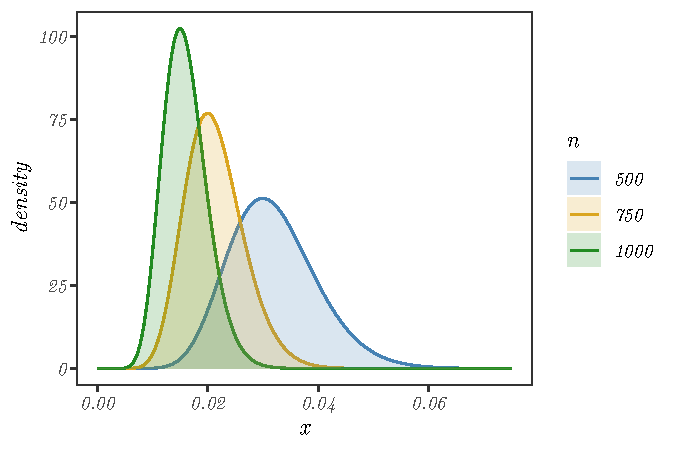
\includegraphics[width=.7\textwidth]{fig/fig-erlang-example-1.pdf}
  \caption[Probability density function of the Erlang distribution]{Probability density function $E(x, k, n+1)$ of the Erlang distribution, with $k=16$ and $n$ either 500, 750, or 1000.}
  \label{fig-erlang-example}
\end{figure}

We can now answer the second question: given $n$ and a confidence
level $\alpha$, what is the threshold value $u$ for $x_k$ such
that the probability that $x_k < u$ is equal to $\alpha$? That is,
we wish to know the value $x = u$ at which the probability
distribution has encompassed a given area of $\alpha$ (see figure~\ref{fig-alpha}).

\begin{figure}[!ht]
  \centering 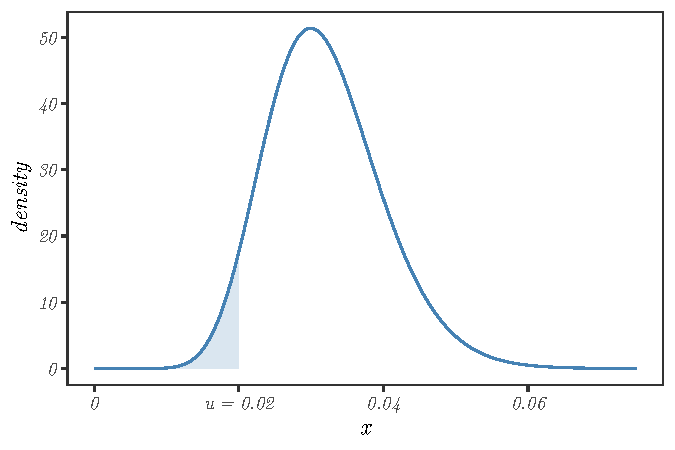
\includegraphics[width=.7\textwidth]{fig/fig-alpha-1.pdf}
  \caption[The 16th smallest value among $500$ random variates on unit interval]{The distribution of $x_{16}$, i.e., the 16th smallest value from among $n=500$ independently and uniformly drawn variates between 0 and 1. The area under the curve is shaded up to 5\% of its area. The point at which the shading stops is therefore the value $u$ for which there is only a 5\% chance of getting an even smaller $x_{16}$.}
  \label{fig-alpha}
\end{figure}

The area under
the curve of the Erlang distribution is given by its cumulative
distribution function $P(x,k,n+1)$, which is known to be
\begin{equation}\protect\hypertarget{eq-Erlang-cdf}{}{
P(x,k,n+1)
= \int_0^x E(y,k,n+1) \,\text{d}y
= \frac{1}{(k-1)!} \int_0^{(n+1)x} t^{k-1}\text{e}^{-t} \,\text{d} t .
}\label{eq-Erlang-cdf}\end{equation} The latter expression is sometimes
written as $\tilde{\gamma}(k,(n+1)x)$, where
\begin{equation}\protect\hypertarget{eq-gamma-regularized}{}{
\tilde{\gamma}(k,x)
= \frac{1}{\Gamma(k)} \int_0^x t^{k-1} \text{e}^{-t} \,\text{d}t
}\label{eq-gamma-regularized}\end{equation} is the regularized lower
incomplete gamma function. We therefore want to solve the equation
\begin{equation}\protect\hypertarget{eq-alpha}{}{
\alpha
= \int_0^u E(y,k,n+1) \,\text{d}y = P(u,k,n+1)
}\label{eq-alpha}\end{equation} for $u$.

Inverting this expression in $u$ (since the cumulative distribution
function increases monotonically in $u$, the inverse exists) leads to
the quantile function $Q(\alpha,k,n+1)$ of the Erlang distribution:
$u = Q(\alpha,k,n+1)$.
The quantile function is known to be expressible as
\begin{equation}\protect\hypertarget{eq-erlang-quantile}{}{
Q(\alpha,k,n+1)
= \frac{\tilde{\gamma}^{-1}(k,x)}{n+1} ,
}\label{eq-erlang-quantile}\end{equation} where
$\tilde{\gamma}^{-1}(k,x)$ is the inverse regularized lower incomplete
gamma function. Its particular form is of no interest to us, except for
two properties. First, it is positive for all $x$.%
%
\footnote{This stands to
reason: the quantile function of a distribution on
$x \in [0, \, \infty)$ is itself between 0 and $\infty$, and
$\tilde{\gamma}^{-1}(k,x)$ is just the quantile function of the Erlang
distribution times the positive constant $n+1$.}
%
Second, it is
independent of $n$. Instead, the entire dependence of
$Q(\alpha,k,n+1)$ on $n$ is given by the $n+1$ term in the
denominator of Equation~\ref{eq-erlang-quantile}. From this, we conclude
that $Q(\alpha,k,n+1)$ is a strictly decreasing function of $n$.

These two points lead to an important consequence. Say we compute the
threshold $u$ for a given $\alpha$ and $n$ in order to have an upper bound on a lower quantile. Now, if we were to
decrease $n$ but hold all other things equal, the threshold will
always get higher than what it was before. The threshold obtained for
higher values of $n$ may therefore serve as a conservative estimate of
the threshold for lower values: if $u$ is a threshold such that the
$k$th smallest out of $n$ uniform variates is only smaller than $u$ in
$\alpha$ of cases, then for any amount $m<n$, the chance of the
$k$th variate conforming to the same constraint (i.e., $x_k<u$) is now even smaller than $\alpha$. 

Conversely, if we were to constrain $x_k$ so that the probability of not getting a value smaller than $u$ is lower than $\beta$ (minimising a higher quantile), we find that the constraint remains true as $n$ is increased.

Armed with these results, let us see how
Equation~\ref{eq-erlang-quantile} can be used for the estimation
procedure.  
There are two problems to tackle, ultimately relating to the two aspects of a test's accuracy. First, we want to catch inadequate storers slacking on volume. In other words, we want to constrain the $x_k$ values so that we can safely say that any attacker with a stored volume below an acceptable size $n$ has a probability less than $\alpha$ to obtain such a small $x_k$ by pure chance. Construing the condition for $x_k<u$ as a test to filter honest players (just based on the size of their reserve), $1-\alpha$ expresses the \emph{sensitivity} of the test.
From the previous argument on the monotonic dependence of $\alpha$ on $n$, it is safe to use a condition that requires $x_k$ to stay below a threshold obtained for $n$. 

Second, we want to avoid situations when honest participants end up not satisfying the above constraint even though they sampled from a set larger than the required minimum. Given a target volume $m>n$, the error rate of false negatives is guaranteed to be less than $\beta$ obtained from the quantile function with parameters $m, k, \text{ and }u$. The quantity $1-\beta$ is the \emph{specificity} or \emph{precision}
of the test.



Figure~\ref{fig-ns} illustrates this
idea, for two different distributions in both the lower- and upper-end
estimation. What we want is to choose $u$ to simultaneously make sure
that dishonest players do not sneak through the system \emph{and} also that
honest players do not get excluded too often. This translates to make both $\alpha$
and $\beta$ as small as possible. 


\begin{figure}[!ht]
  \centering
  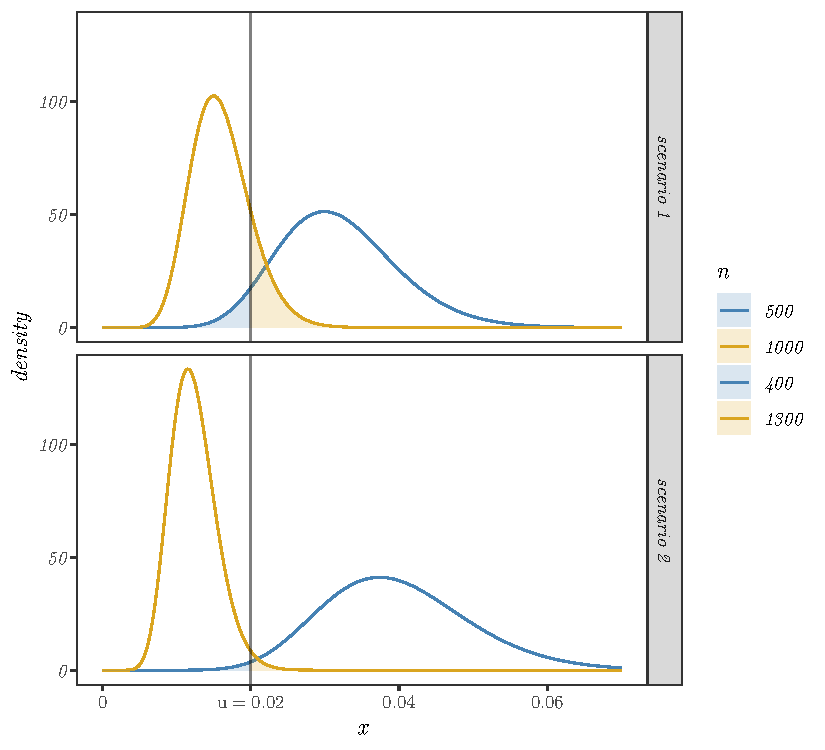
\includegraphics[width=.7\textwidth]{fig/fig-ns-1.pdf}
  \caption[Recall and precision of proof of reserve size validation]{Recall and precision of proof of reserve size validation: Any chosen $u$ will lead to different $\alpha$ and $\beta$ values, depending on $n$. Here $u$ is fixed at $0.02$. The top panel shows distributions for $x \equiv x_{16}$ with $n = 500$ (blue) and $n = 1000$ (yellow). The area left under the blue curve to the left of $u$ is equal to $\alpha$ (blue shade); the area under the yellow curve right of $u$ is equal to $\beta$ (yellow shade). If the curves overlap considerably (top), it is impossible to choose an $u$ such that $\alpha$ and $\beta$ are simultaneously small.}
  \label{fig-ns}
\end{figure}


One way to try and find the best compromise is by minimising
$\alpha + \beta$ (the \emph{accuracy} of the test) and pick the $u$ value at the optimum to be used in the proof of resources test. To this end, one
can vary $\alpha$ between 0 and 1 and, for each of its values, solve
the equation $\alpha = Q(1-\beta, k, n+1)$ (where $n$ is the larger
value, used for estimating $\beta$). This way, we get a $\beta$
value for every possible $\alpha$. Then, we can find the combination
which minimises $\alpha + \beta$, and determine the value of $u$
that leads to this optimum. As illustrated in
figure~\ref{fig-optim}, larger values of $k$ yield a trade-off curve along which
better accuracies can be achieved.

\begin{figure}[!ht]
  \centering
  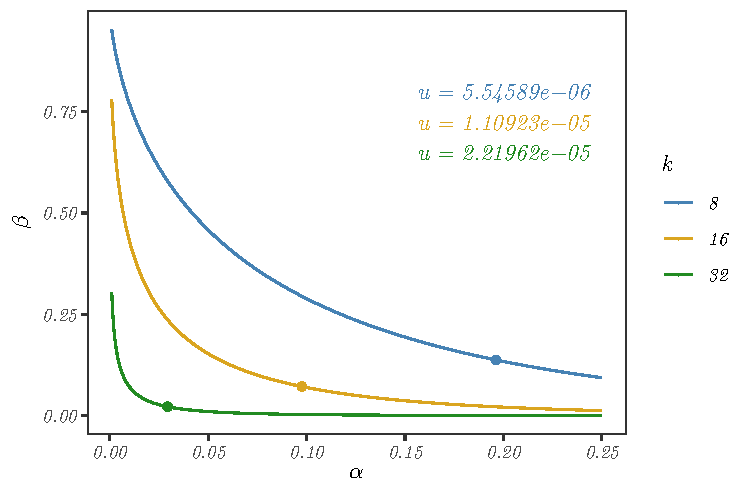
\includegraphics[width=.7\textwidth]{fig/fig-optim-1.pdf}
  \caption[Optimal accuracy of reserve size probe]{Optimal accuracy of reserve size probe By increasing $k$, one can get better optima for minimising $\alpha + \beta$. Here $n = 10^6$ for estimating $\alpha$ and $2\cdot 10^6$ for estimating $\beta$, and $k$ is either 8, 16, or 32 (colors). The values of $u$ associated with the optima are also shown.}
  \label{fig-optim}
\end{figure}



Table~\ref{tab:estim} summarizes the important numerical results in
Figure~\ref{fig-optim}.%
%
\footnote{Since the hash function used to generate random
variates does so in the range $[0, \, 2^{256}-1]$ instead of
$[0, \, 1]$, the calculated thresholds are scaled with $2^{256}$ to
show where they would fall in their actual range.}


\begin{table}[!ht]
 \centering
  \begin{tabular}{rrrrr}
  \toprule
  $k$ & $\alpha$ & $\beta$ & $u$ & $u \cdot 2^{256}$ \\
  \midrule
  8 & 0.196216 & 0.1373622 & $5.54589\cdot 10^{-6}$ & $6.421705\cdot 10^{71}$\\
  16 & 0.097612 & 0.0716570 & $1.10923\cdot 10^{-5}$ & $1.284401\cdot 10^{72}$\\
  32 & 0.029386 & 0.0219151 & $2.21962\cdot 10^{-5}$ & $2.570140\cdot 10^{72}$\\
  \bottomrule
  \end{tabular}
   \caption[Proof of density parameter calibration]{Proof of density parameter calibration. Assuming $n = 10^6$ and $m=2\cdot 10^6$ to calculate recall and precision error rates $\alpha$ and $\beta$, respectively, the cutoff value for the proof is calibrated by optimizing on acccuracy using sample sizes $8, 16, 32$.}
  \label{tab:estim}
\end{table}

\section{Batch utilisation}\label{sec:batch-utilisation}


When pushing content to the Swarm network, uploaders are required to
attach an attestation of storage rent prepayment to each chunk they
post. The latter is essentially a wallet registered on the postage
contract seeded with a balance from which storage rent is deduced by the
network-wide incentive system. Since this is reminiscent of buying a
batch of postage stamps and attaching one to each envelope to be posted,
the attestations are called \emph{postage stamps} and the registered
wallet a \emph{postage batch.} One can think of batches as collections
of \emph{storage slots.} The size of a batch is the number of storage
slots and is always specified as a power of 2, with the exponent
called \emph{batch depth.} Each slot can hold at most one chunk.
Putting a chunk into a slot is like issuing a postage stamp.

In practice, the attached postage stamps are digital signatures which
associate the address of a chunk with a \emph{storage slot reference.}
This in turn is composed of 1) a reference to the wallet through its
\emph{batch ID,} and 2) a \emph{within-batch index.} The fact that each
slot can hold at most one chunk ensures that batches cannot issue more
stamps than the volume registered with them. However, for an
\emph{overissuance} incident to be detectable locally by storer nodes,
the within-batch indices are arranged such that the highest $n$ bits
match the prefix of the chunk they are assigned to. These $n$ bits
define $2^n$ \emph{buckets}, the other half of the index is essentially a counter within the buckets, which is
sequentially assigned to chunks. If
the batch depth is $d$ and there
are $2^n$ buckets, then each bucket will hold a maximum of $2^{d-n}$
chunks. $k=d-n$, the log size of a bucket is called
\emph{bucket depth}. The bucket size ($2^k$) provides an exclusive upper bound to
within-bucket indices. This enforces a uniformity of stamp issuance across the $2^n$ buckets, therefore $n$ is called \emph{uniformity depth}.

Overusing a batch is now easily detected by any storer node as long as
their storage depth is shallower than the batch's uniformity depth. In
that case, each bucket of a batch is entirely within the node's reserve.
Overissuance is therefore immediately caught, since the multiple chunks 
assigned to the same slot index are seen by any node in that
neighbourhood.

When all slots are filled, we say the batch is \emph{fully utilised.} 
Although the \emph{a priori} distribution of chunks is uniform (and
therefore the expected number of chunks falling into each bucket is the
same), their stochastic assignment means that there is necessarily some variance. 
It is practically
impossible to fully fill all buckets before eventually attempting to add to one that is already full. 
We assume that the uploader is unable to
affect the address of the chunks (unencrypted fixed content) so in this scenario they are unable to
continue uploading. Because of this, one may legitimately consider the
batch to be no longer usable. The number of stamps hitherto issued by
the batch is called its \emph{effective batch size,} and its ratio to
the batch size its \emph{batch utilization rate.}

Below we explore the effect of batch parameters on their utilization
rate. With an insight into utilization rates as a function of the number
of buckets $2^n$ and the size of buckets $2^k$, we will have a way
to calibrate the expected effective batch size to be presented to users
in the context of a batch purchase user experience.

The problem of assigning chunks to storage slots is analogous with the
process of throwing marbles, one after the other, in boxes which are
initially empty. Each throw may end up in any of the boxes with equal
probability, and thus the marbles get distributed across the boxes more
or less evenly through time. However, the time will come when the boxes
start filling up. At that point, a marble may by chance end up being
thrown into a box that is already full, and thus get rejected.
Substituting chunks for marbles, buckets for boxes, and the act of
signing a stamp for throwing a marble, we recover our original scenario.
Marbles ending up in a box with equal probability corresponds to the
fact that a random chunk has equal chance of being assigned to a bucket
since the hash function has uniform distribution. Repeated rounds of
marble throwing correspond to consecutive stamping of multiple chunks of
the uploaded content; rounds constitute repeated independent trials.

Taking a particular bucket, each round of stamping is a ``success'' if
the stamp falls into the bucket, and a ``failure'' otherwise. Due to the
fact that a marble may end up in each box with equal chance, the
probability of success is $1/n$ and the probability of failure is
$1 - 1/n$. The number of stamps issued to the bucket after a given
number of rounds is described by the
\href{https://en.wikipedia.org/wiki/Negative_binomial_distribution\#Distribution_of_a_sum_of_geometrically_distributed_random_variables}{negative
binomial distribution} $\mathcal{B}(k, 1/n)$, where the first
parameter $k$ is the number of failed rounds before we stop counting,
and the second parameter is the probability of success.

The negative binomial distribution $\mathcal{B}(k, 1/n)$ is equivalent
to the sum of $k$ independent geometrically distributed variables with
parameter $1/n$. Unless $k$ is very small, the central limit theorem
ensures that this sum converges to a normal distribution. Formally, if
$\mathcal{Y}_i(1/n)$ are independent geometrically distributed
variables with parameter $1/n$, and $\mathcal{N}(\mu, \sigma^2)$ is
the normal distribution with mean $\mu$ and variance $\sigma^2$,
then for large $k$ we have
\begin{equation}\protect\hypertarget{eq-binomial-approximation}{}{
\mathcal{B}(k, 1/n) = \sum_{i=1}^k \mathcal{Y}_i(1/n) \approx \mathcal{N}(kn, kn(n-1))
}\label{eq-binomial-approximation}\end{equation} The reason for the
above form of the mean and variance in the normal distribution is as
follows: given a single geometrically distributed variable with
parameter $1/n$, its mean is $n$ and its variance is $n(n-1)$.
When adding these up over $k$ independent variables, we arrive at
$\mu = k n$ and $\sigma^2 = k n (n - 1)$ in the limiting normal
distribution.

The fit of the normal distribution with the negative binomial is robust even for
low values of $k$, as depicted in Figure~\ref{fig-normal-binomial}.

\begin{figure}
  \centering
  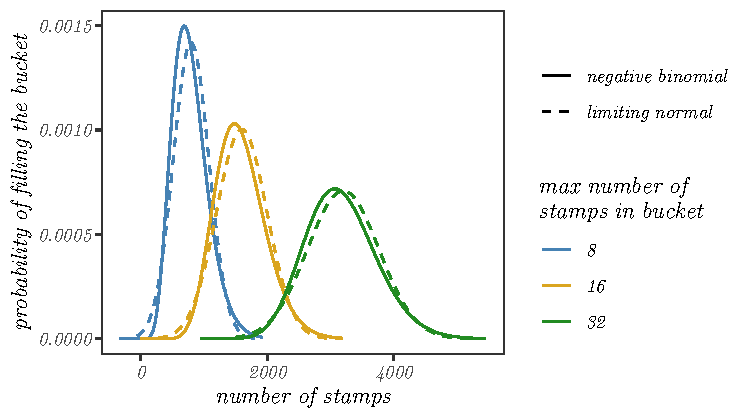
\includegraphics[width=0.7\textwidth]{postage_batch_utilization_figs/fig-normal-binomial-1.pdf}
  \caption[Approximating negative binomial]{\label{fig-normal-binomial}Approximating negative binomial distributions with limiting normal ones. The number of buckets $n$ is fixed at 100.}
\end{figure}

The negative binomial distribution estimates the number of rounds a
particular bucket fills up, given its size $k$ and the number of
buckets $n$. The rounds of stamping can be conceived of as parallel
independent attempts at filling up buckets. Stamps issued for failed
rounds still end up in one of the other $n - 1$ buckets, and therefore
the same probability variable counts the total stamps issued by the
batch in all buckets at the time the first one fills up. Thus, we want
to know how the \emph{minimum} of $n$ independent normal variates,
$X = \min_{i \in \{1\ldots n\}} \mathcal{N}_i(\mu, \sigma^2)$, is
distributed.

This so-called \emph{extreme value distribution} would give us the
distribution of the absolute number of total rounds needed until the
first event when one of the buckets fills up. Therefore its mean is
exactly the expected value of the number of rounds until the first
bucket-filling event. Since this is when the batch is considered
effectively used up, the mean of the distribution measures the effective
utilization of the batch. Dividing by $n$ gives the expected number of
stamps per bucket making the rate comparable across any parameter of
bucket size. Further dividing by $k$ in turn gives the \emph{expected
normalized utilization rate}, which is now comparable across all $k$
and $n$ values.

The extreme value distribution for the minimum of $n$ independent
variates drawn from the standard normal distribution (with zero mean and
unit variance) is known. It is the
\href{https://en.wikipedia.org/wiki/Gumbel_distribution}{Gumbel
distribution}, which reads
\begin{equation}\protect\hypertarget{eq-gumbel}{}{
\mathcal{G}(x; \alpha, \beta) = \frac{1}{\beta} \exp\left[
\frac{x + \alpha}{\beta} - \exp\left(\frac{x + \alpha}{\beta}\right)\right] .
}\label{eq-gumbel}\end{equation} Here $x$ is the independent variable
(in our case, the number of rounds of stamping), and $\alpha$ and
$\beta$ are the \emph{location} and \emph{scale} parameters,
respectively.\footnote{The Gumbel distribution is often given using the
  convention that one is looking for the maximum of $n$ normal
  variates, instead of their minimum. One can change between the two by
  simply flipping the sign of $x$.} They are in turn given by
\begin{equation}\protect\hypertarget{eq-loc-scale}{}{
\begin{aligned}
  \alpha &= \rho\left( 1 - \frac{1}{n} \right) ,
  \\
  \beta &= \rho\left( 1 - \frac{\text{e}^{-1}}{n} \right) - \alpha ,
\end{aligned}
}\label{eq-loc-scale}\end{equation} where
$\text{e}^{-1} = \exp(-1) \approx 0.368$, $n$ is the number of
normal variates whose minimum we are looking for, and $\rho(x)$ is the
quantile function of the normal distribution (or the inverse of the
\href{https://en.wikipedia.org/wiki/Error_function}{error function}).
The mean, standard deviation, and quantile function of the Gumbel
distribution are
\begin{equation}\protect\hypertarget{eq-mean-var-quantile}{}{
\begin{aligned}
  \mathbb{E}(\mathcal{G}) &= \alpha + \gamma \beta ,
  \\
  \mathbb{S}(\mathcal{G}) &= \beta \, \frac{\pi}{\sqrt{6}} ,
  \\
  Q(p; \mathcal{G}) &= \beta \, \log(-\log(1 - p)) - \alpha ,
\end{aligned}
}\label{eq-mean-var-quantile}\end{equation} where
$\gamma \approx 0.5772$ is the Euler--Mascheroni constant, and
$0 < p < 1$ in $Q(p; \mathcal{G})$ is a probability quantile.

The normal distribution whose variates' minimum values we are looking
for is not standard, but instead has mean $\mu = k n$ (instead of
zero), and variance $\sigma^2 = k n (n-1)$ (instead of one).
Therefore, the Gumbel distribution needs to be appropriately rescaled.
Denoting this scaled probability distribution by $\mathcal{X}$, we
have \begin{equation}\protect\hypertarget{eq-gumbel-scaled}{}{
  \mathcal{X}(x; \mu, \sigma, \alpha, \beta) =
  \frac{1}{\sigma}\mathcal{G}\left(\frac{x - \mu}{\sigma}; \alpha, \beta\right)
}\label{eq-gumbel-scaled}\end{equation} (the overall factor of
$1 / \sigma$ restores the proper normalization of the scaled
function). Consequently, the mean, standard deviation, and quantile
function should also be rescaled:
\begin{equation}\protect\hypertarget{eq-mean-var-quantile-scaled}{}{
\begin{aligned}
  \mathbb{E}(\mathcal{X}) &= \mu - \sigma (\alpha+\gamma\beta) = kn-\sqrt{kn(n-1)}
  \left[(1-\gamma) \rho\left( 1 - \frac{1}{n} \right) + \gamma \rho\left( 1 -
  \frac{\text{e}^{-1}}{n} \right) \right] , 
  \\
  \mathbb{S}(\mathcal{X}) &=\sigma \beta \frac{\pi}{\sqrt{6}} =
  \sqrt{ k n (n-1)} \left[ \rho\left( 1 - \frac{\text{e}^{-1}}{n} \right) -
  \rho\left( 1 - \frac{1}{n} \right) \right] \frac{\pi}{\sqrt{6}} ,
  \\
  Q(p;\mathcal{X})&= \mu-\sigma\left[\alpha-\beta \,
  \log(-\log(1-p))\right] \\ &= kn-\sqrt{ k n (n-1)}\left[\rho\left( 1 -
  \frac{1}{n} \right)-\rho\left( 1 - \frac{\text{e}^{-1}}{n} \right) 
  \log\left(-\log(1-p)\right)\right] .
\end{aligned}
}\label{eq-mean-var-quantile-scaled}\end{equation} Normalizing the mean
and the quantile function by the product $kn$:
\begin{equation}\protect\hypertarget{eq-mean-quant-div}{}{
\begin{aligned}
  \frac{\mathbb{E}(\mathcal{X})}{k n} &= 1 - \sqrt{\frac{(n-1)}{kn}} \left[ (1-\gamma)
  \rho\left( 1 - \frac{1}{n} \right) + \gamma \rho\left( 1 - \frac{\text{e}^{-1}}{n}
  \right) \right] ,
  \\
  \frac{Q(p; \mathcal{X})}{kn} &= 1 - \sqrt{\frac{(n-1)}{kn}}
  \left[\rho\left( 1 - \frac{1}{n} \right)-\rho\left( 1 - \frac{\text{e}^{-1}}{n}
  \right)  \log\left(-\log(1-p)\right)\right] .
\end{aligned}
}\label{eq-mean-quant-div}\end{equation} Taking into account that $k$
and $n$ must both be powers of two, we can write $k = 2^{\kappa}$
and $n = 2^{\nu}$, where $\kappa$ and $\nu$ are positive integers.
We then have \begin{equation}\protect\hypertarget{eq-mean-div-simp}{}{
  \frac{\mathbb{E}(\mathcal{X})}{k n} =
  \frac{\mathbb{E}(\mathcal{X})}{2^{\kappa + \nu}} =
  1 - \sqrt{\frac{2^\nu-1}{2^{\kappa+\nu}}}\left[ (1-\gamma) \rho\left( 1 -
  \frac{1}{2^{\nu}} \right) + \gamma \rho\left( 1 - \frac{\text{e}^{-1}}{2^{\nu}}
  \right) \right] .
}\label{eq-mean-div-simp}\end{equation}

In order to explore this solution, we consider the average expected
utilization rate as a function of uniformity depth, for various log bucket
sizes (see Figure~\ref{fig-mean}). As long as bucket size is around $2^8$ or greater,
the dependence of the utilization rate on $n$ is milder and milder, and at $2^{16}$, it is virtually a flat line at $100\%$.
In general, we see that for the same bucket size, the miss rate
(one minus the utilization rate) increases with the number of buckets. Using
small bucket sizes (up to $2^{10}$), we get unacceptably high miss
rates even with few buckets.%
%
\footnote{Note that for low $k$ but high
  $n$, the solution is unreliable, predicting a negative number of
  stamps per bucket. The prediction will generally not work well if
  $k$ is too small, because the normal approximation to the negative
  binomial distribution starts to break down.}
%  
On the other hand, for
larger bucket sizes (over $2^{10}$), the miss rate is contained at a
tolerable $<10\%$ (on the right in Figure~\ref{fig-mean}).

On the right, we plot the miss rate on a logarithmic scale as a function of log bucket size, for various numbers of buckets. We
find that doubling the batch size 6 times decreases the miss rate
tenfold, regardless the actual size or the number of buckets. In fact,
as the close parallel lines show (on the right in Figure~\ref{fig-mean}), there is no interaction:
going from one bucket to a billion increases the miss rate
only by tenfold, independently of bucket size.


\begin{figure}[!ht]
  \centering
  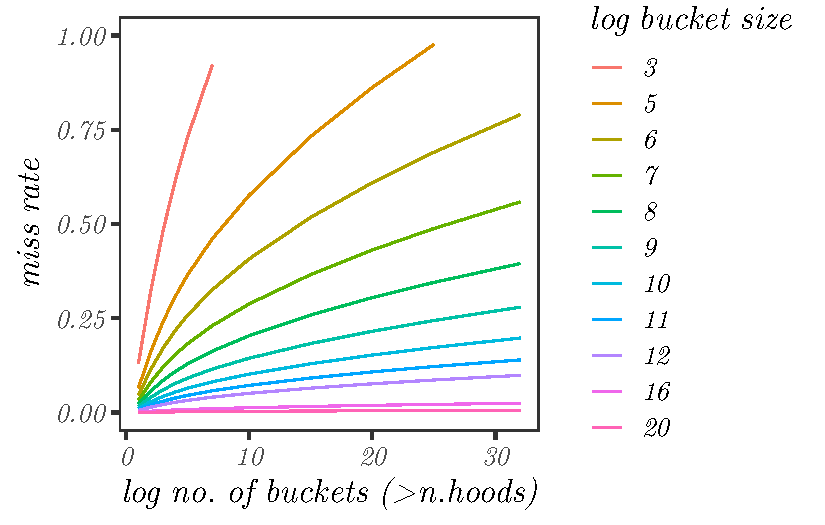
\includegraphics[width=0.49\textwidth]{postage_batch_utilization_figs/fig-mean-1.pdf} 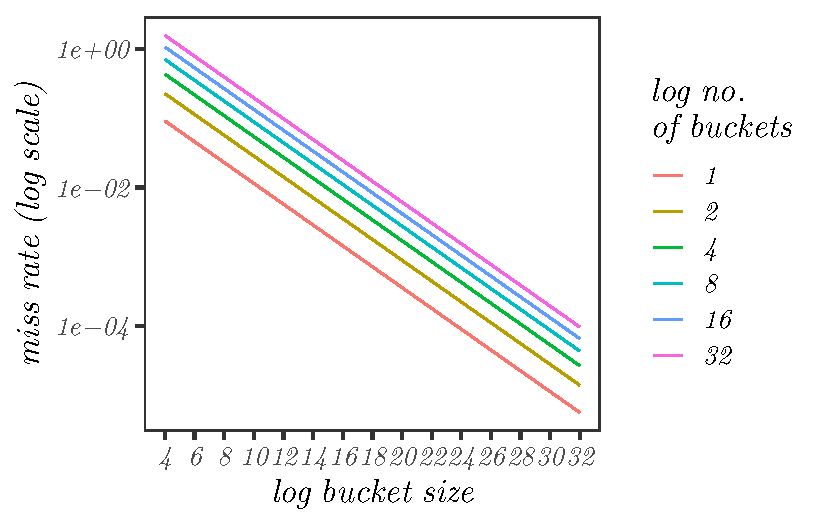
\includegraphics[width=0.49\textwidth]{postage_batch_utilization_figs/fig-mean-2.pdf}
  \caption[Expected miss rate, for various parameters.]{\label{fig-mean}Expected miss rate, for various parameters. Left: miss rate against the number of buckets. Right: miss rate against bucket size.}
\end{figure}


\begin{figure}[!ht]
  \centering
  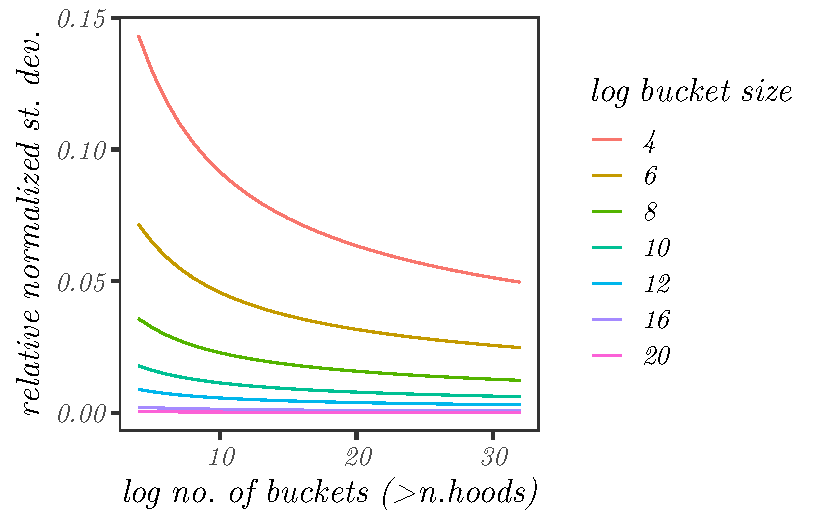
\includegraphics[width=0.49\textwidth]{postage_batch_utilization_figs/fig-sd-1.pdf} 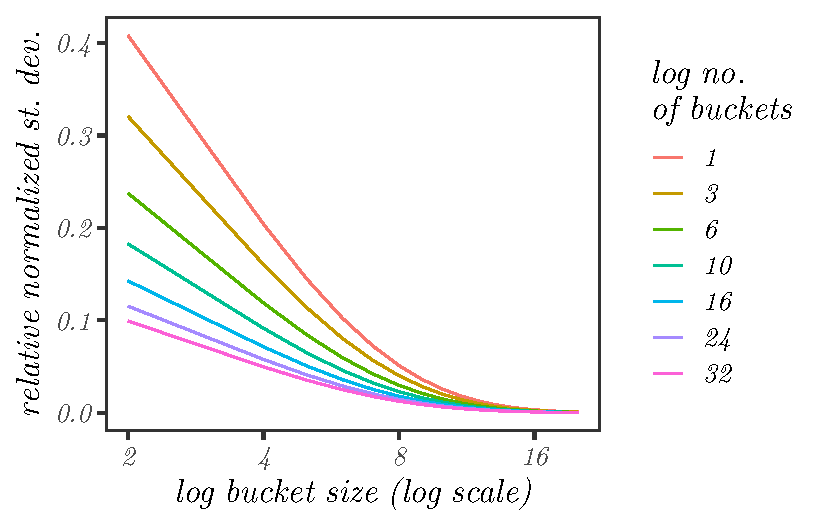
\includegraphics[width=0.49\textwidth]{postage_batch_utilization_figs/fig-sd-2.pdf}
  \caption[Normalized standard deviation of utilization rate]{\label{fig-sd}Normalized standard deviation of utilization rate, for various parameters. Left: relative standard deviation against the number of buckets. Right: relative standard deviation against bucket size.}
\end{figure}




Looking at relative standard deviation of the distribution for various values of $k$ and $n$ (see Figure~\ref{fig-sd}), we find not much variance whenever $k$ and $n$ are large. Nevertheless, for the sake of correctness, we check the quantile function of our extreme value distribution (see Figures~\ref{fig-qua} and \ref{fig-q}).

\begin{figure}[!ht]
  \centering
  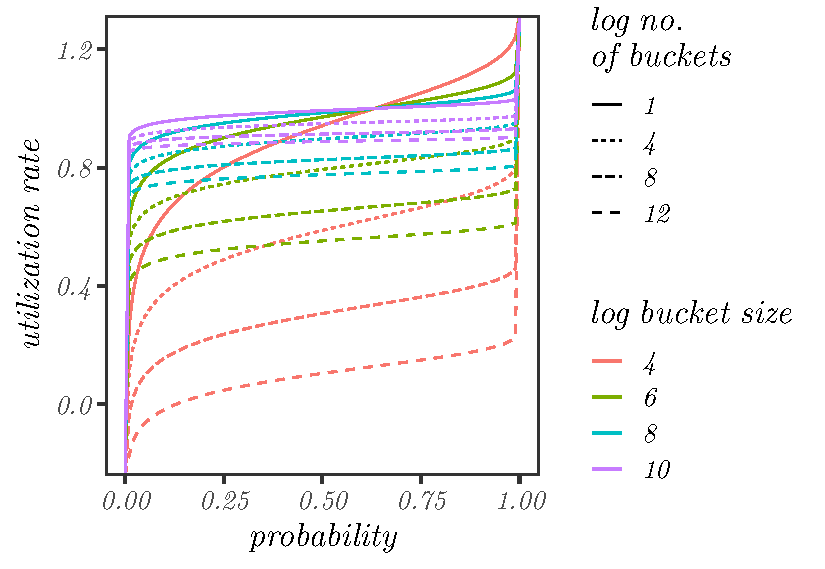
\includegraphics[width=0.49\textwidth]{postage_batch_utilization_figs/fig-qua-1.pdf} 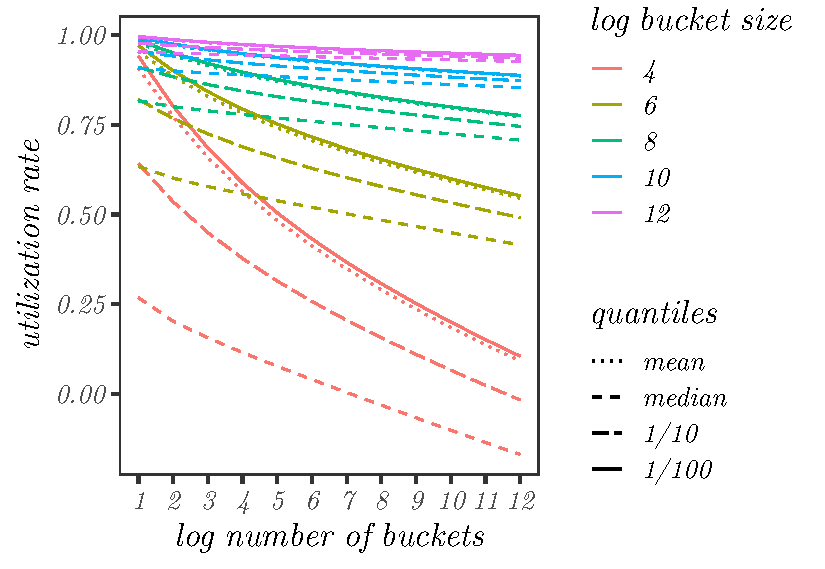
\includegraphics[width=0.49\textwidth]{postage_batch_utilization_figs/fig-qua-2.pdf}
  \caption[Quantiles of the utilization rate]{\label{fig-qua}Quantiles of the utilization rate, for
various parameters. Left: the quantile function of the utilization
rate. Right: mean, median, 10\%, and 1\% percentiles of utilization against the number of buckets.}
\end{figure}

\begin{figure}[!ht]
  \centering
  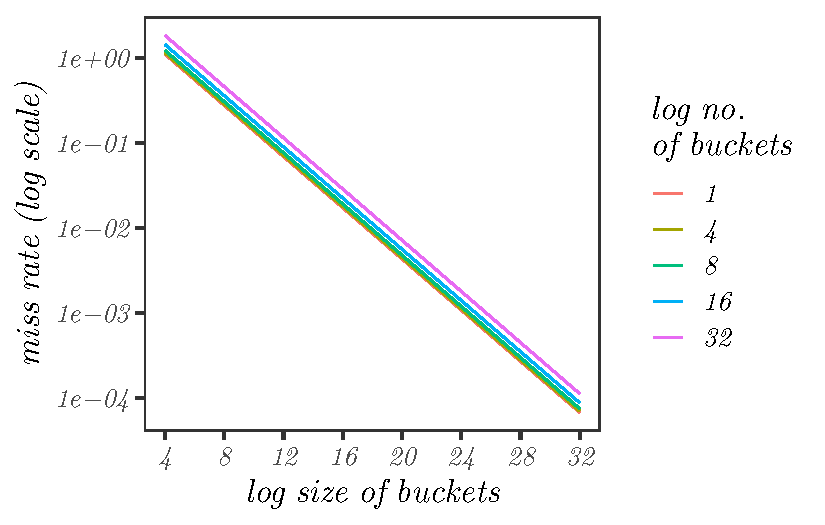
\includegraphics[width=0.49\textwidth]{postage_batch_utilization_figs/fig-q-1.pdf} 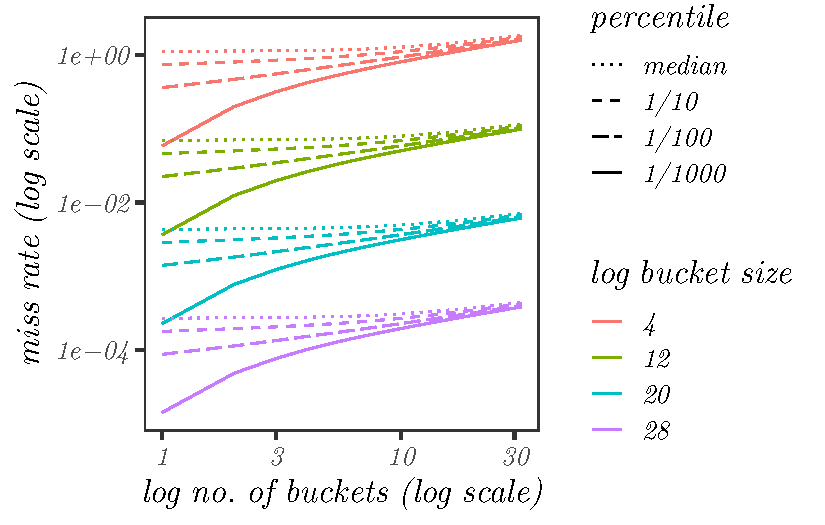
\includegraphics[width=0.49\textwidth]{postage_batch_utilization_figs/fig-q-2.pdf}
  \caption[Quantiles of the miss rate]{Quantiles of the miss rate for various parameters. Left: one-in-a-thousand quantile for miss rate against bucket size. Right: miss rate in terms of percentiles, against number of buckets.}
\label{fig-q}
\end{figure}


Eventually, we aim to use the information on utilization rates to
protect the user from being surprised at the effective utilization of
their postage batch. To this end, we apply the volume calibration using
a reasonable worst-case scenario, i.e., define the effective utilization
rate as the one-in-a-thousand low-tail quantile of the utilization rate.
To obtain the ``effective'' volumes, we simply multiply the theoretical
purchased volume (given by $2^d$ where $d$ is the batch depth) by
the effective utilization rate.


Finally, in table~\ref{tab:batch-utilisation}, we provide these volume calibrations for $2^{12}$ and
$2^{16}$ buckets and log bucket sizes ranging from $4$ to $25$.
Above this bucket size the required quantile already shows a miss rate
below $0.1\%$. That is, there is only a one-in-a-thousand chance that
the difference between the effectively utilized volume and the
theoretically purchased one exceeds one tenth of a percent which we
consider insignificant enough to justify no calibration on the
theoretical volume.

\newpage

\begin{longtable}{rrrrrr}\toprule
\multicolumn{1}{c}{log2 no.}& 
\multicolumn{1}{c}{log2 size} & 
\multicolumn{1}{c}{log2 no.}&
\multicolumn{1}{c}{utilisation}&
\multicolumn{1}{c}{theoretical}&
\multicolumn{1}{c}{effective}\\
\multicolumn{1}{c}{of buckets}&
\multicolumn{1}{c}{of buckets}&
\multicolumn{1}{c}{of chunks}&
\multicolumn{1}{c}{rate}&
\multicolumn{1}{c}{volume}&
\multicolumn{1}{c}{volume}\\
\midrule
12 & 4 & 16 & 0.00000 & 268.44 MB & 0.00 B \\
12 & 5 & 17 & 0.06747 & 536.87 MB & 36.22 MB \\
12 & 6 & 18 & 0.34060 & 1.07 GB & 365.72 MB \\
12 & 7 & 19 & 0.53374 & 2.15 GB & 1.15 GB \\
12 & 8 & 20 & 0.67030 & 4.29 GB & 2.88 GB \\
12 & 9 & 21 & 0.76687 & 8.59 GB & 6.59 GB \\
12 & 10 & 22 & 0.83515 & 17.18 GB & 14.35 GB \\
12 & 11 & 23 & 0.88343 & 34.36 GB & 30.35 GB \\
12 & 12 & 24 & 0.91758 & 68.72 GB & 63.06 GB \\
12 & 13 & 25 & 0.94172 & 137.44 GB & 129.43 GB \\
12 & 14 & 26 & 0.95879 & 274.88 GB & 263.55 GB \\
12 & 15 & 27 & 0.97086 & 549.76 GB & 533.74 GB \\
12 & 16 & 28 & 0.97939 & 1.10 TB & 1.08 TB \\
12 & 17 & 29 & 0.98543 & 2.20 TB & 2.17 TB \\
12 & 18 & 30 & 0.98970 & 4.40 TB & 4.35 TB \\
12 & 19 & 31 & 0.99271 & 8.80 TB & 8.73 TB \\
12 & 20 & 32 & 0.99485 & 17.59 TB & 17.50 TB \\
12 & 21 & 33 & 0.99636 & 35.18 TB & 35.06 TB \\
12 & 22 & 34 & 0.99742 & 70.37 TB & 70.19 TB \\
12 & 23 & 35 & 0.99818 & 140.74 TB & 140.48 TB \\
12 & 24 & 36 & 0.99871 & 281.47 TB & 281.11 TB \\
12 & 25 & 37 & 0.99909 & 562.95 TB & 562.44 TB \\
16 & 4 & 20 & 0.00000 & 4.29 GB & 0.00 B \\
16 & 5 & 21 & 0.00000 & 8.59 GB & 0.00 B \\
16 & 6 & 22 & 0.28669 & 17.18 GB & 4.93 GB \\
16 & 7 & 23 & 0.49561 & 34.36 GB & 17.03 GB \\
16 & 8 & 24 & 0.64334 & 68.72 GB & 44.21 GB \\
16 & 9 & 25 & 0.74781 & 137.44 GB & 102.78 GB \\
16 & 10 & 26 & 0.82167 & 274.88 GB & 225.86 GB \\
16 & 11 & 27 & 0.87390 & 549.76 GB & 480.43 GB \\
16 & 12 & 28 & 0.91084 & 1.10 TB & 1.00 TB \\
16 & 13 & 29 & 0.93695 & 2.20 TB & 2.06 TB \\
16 & 14 & 30 & 0.95542 & 4.40 TB & 4.20 TB \\
16 & 15 & 31 & 0.96848 & 8.80 TB & 8.52 TB \\
16 & 16 & 32 & 0.97771 & 17.59 TB & 17.20 TB \\
16 & 17 & 33 & 0.98424 & 35.18 TB & 34.63 TB \\
16 & 18 & 34 & 0.98885 & 70.37 TB & 69.58 TB \\
16 & 19 & 35 & 0.99212 & 140.74 TB & 139.63 TB \\
16 & 20 & 36 & 0.99443 & 281.47 TB & 279.91 TB \\
16 & 21 & 37 & 0.99606 & 562.95 TB & 560.73 TB \\
16 & 22 & 38 & 0.99721 & 1.13 PB & 1.12 PB \\
16 & 23 & 39 & 0.99803 & 2.25 PB & 2.25 PB \\
16 & 24 & 40 & 0.99861 & 4.50 PB & 4.50 PB \\
16 & 25 & 41 & 0.99901 & 9.01 PB & 9.00 PB \\
\bottomrule
\caption{Theoretical and effective volumes of postage batches}
\label{tab:batch-utilisation}
\end{longtable}


\end{document}



